% Options for packages loaded elsewhere
\PassOptionsToPackage{unicode}{hyperref}
\PassOptionsToPackage{hyphens}{url}
\PassOptionsToPackage{dvipsnames,svgnames,x11names}{xcolor}
%
\documentclass[
  11pt,
]{book}
\usepackage{amsmath,amssymb}
\usepackage{iftex}
\ifPDFTeX
  \usepackage[T1]{fontenc}
  \usepackage[utf8]{inputenc}
  \usepackage{textcomp} % provide euro and other symbols
\else % if luatex or xetex
  \usepackage{unicode-math} % this also loads fontspec
  \defaultfontfeatures{Scale=MatchLowercase}
  \defaultfontfeatures[\rmfamily]{Ligatures=TeX,Scale=1}
\fi
\usepackage{lmodern}
\ifPDFTeX\else
  % xetex/luatex font selection
\fi
% Use upquote if available, for straight quotes in verbatim environments
\IfFileExists{upquote.sty}{\usepackage{upquote}}{}
\IfFileExists{microtype.sty}{% use microtype if available
  \usepackage[]{microtype}
  \UseMicrotypeSet[protrusion]{basicmath} % disable protrusion for tt fonts
}{}
\makeatletter
\@ifundefined{KOMAClassName}{% if non-KOMA class
  \IfFileExists{parskip.sty}{%
    \usepackage{parskip}
  }{% else
    \setlength{\parindent}{0pt}
    \setlength{\parskip}{6pt plus 2pt minus 1pt}}
}{% if KOMA class
  \KOMAoptions{parskip=half}}
\makeatother
\usepackage{xcolor}
\usepackage[margin=1in]{geometry}
\usepackage{longtable,booktabs,array}
\usepackage{calc} % for calculating minipage widths
% Correct order of tables after \paragraph or \subparagraph
\usepackage{etoolbox}
\makeatletter
\patchcmd\longtable{\par}{\if@noskipsec\mbox{}\fi\par}{}{}
\makeatother
% Allow footnotes in longtable head/foot
\IfFileExists{footnotehyper.sty}{\usepackage{footnotehyper}}{\usepackage{footnote}}
\makesavenoteenv{longtable}
\usepackage{graphicx}
\makeatletter
\def\maxwidth{\ifdim\Gin@nat@width>\linewidth\linewidth\else\Gin@nat@width\fi}
\def\maxheight{\ifdim\Gin@nat@height>\textheight\textheight\else\Gin@nat@height\fi}
\makeatother
% Scale images if necessary, so that they will not overflow the page
% margins by default, and it is still possible to overwrite the defaults
% using explicit options in \includegraphics[width, height, ...]{}
\setkeys{Gin}{width=\maxwidth,height=\maxheight,keepaspectratio}
% Set default figure placement to htbp
\makeatletter
\def\fps@figure{htbp}
\makeatother
\setlength{\emergencystretch}{3em} % prevent overfull lines
\providecommand{\tightlist}{%
  \setlength{\itemsep}{0pt}\setlength{\parskip}{0pt}}
\setcounter{secnumdepth}{5}
\usepackage{booktabs}
\ifLuaTeX
  \usepackage{selnolig}  % disable illegal ligatures
\fi
\usepackage[]{natbib}
\bibliographystyle{plainnat}
\usepackage{bookmark}
\IfFileExists{xurl.sty}{\usepackage{xurl}}{} % add URL line breaks if available
\urlstyle{same}
\hypersetup{
  pdftitle={Transforming Research Methods in Health Services Psychology: Applications for the Advocate \textasciitilde{} Practitioner \textasciitilde{} Scientist},
  pdfauthor={Lynette H. Bikos, PhD, ABPP \& Cirleen DeBlaere, PhD, Editors; Kiana Clay, Editorial Assistant},
  colorlinks=true,
  linkcolor={Maroon},
  filecolor={Maroon},
  citecolor={Blue},
  urlcolor={blue},
  pdfcreator={LaTeX via pandoc}}

\title{Transforming Research Methods in Health Services Psychology: Applications for the Advocate \textasciitilde{} Practitioner \textasciitilde{} Scientist}
\author{Lynette H. Bikos, PhD, ABPP \& Cirleen DeBlaere, PhD, Editors \and Kiana Clay, Editorial Assistant}
\date{30 Jan 2025}

\begin{document}
\maketitle

{
\hypersetup{linkcolor=}
\setcounter{tocdepth}{3}
\tableofcontents
}
\chapter*{BOOK COVER}\label{book-cover}


\begin{figure}
\centering
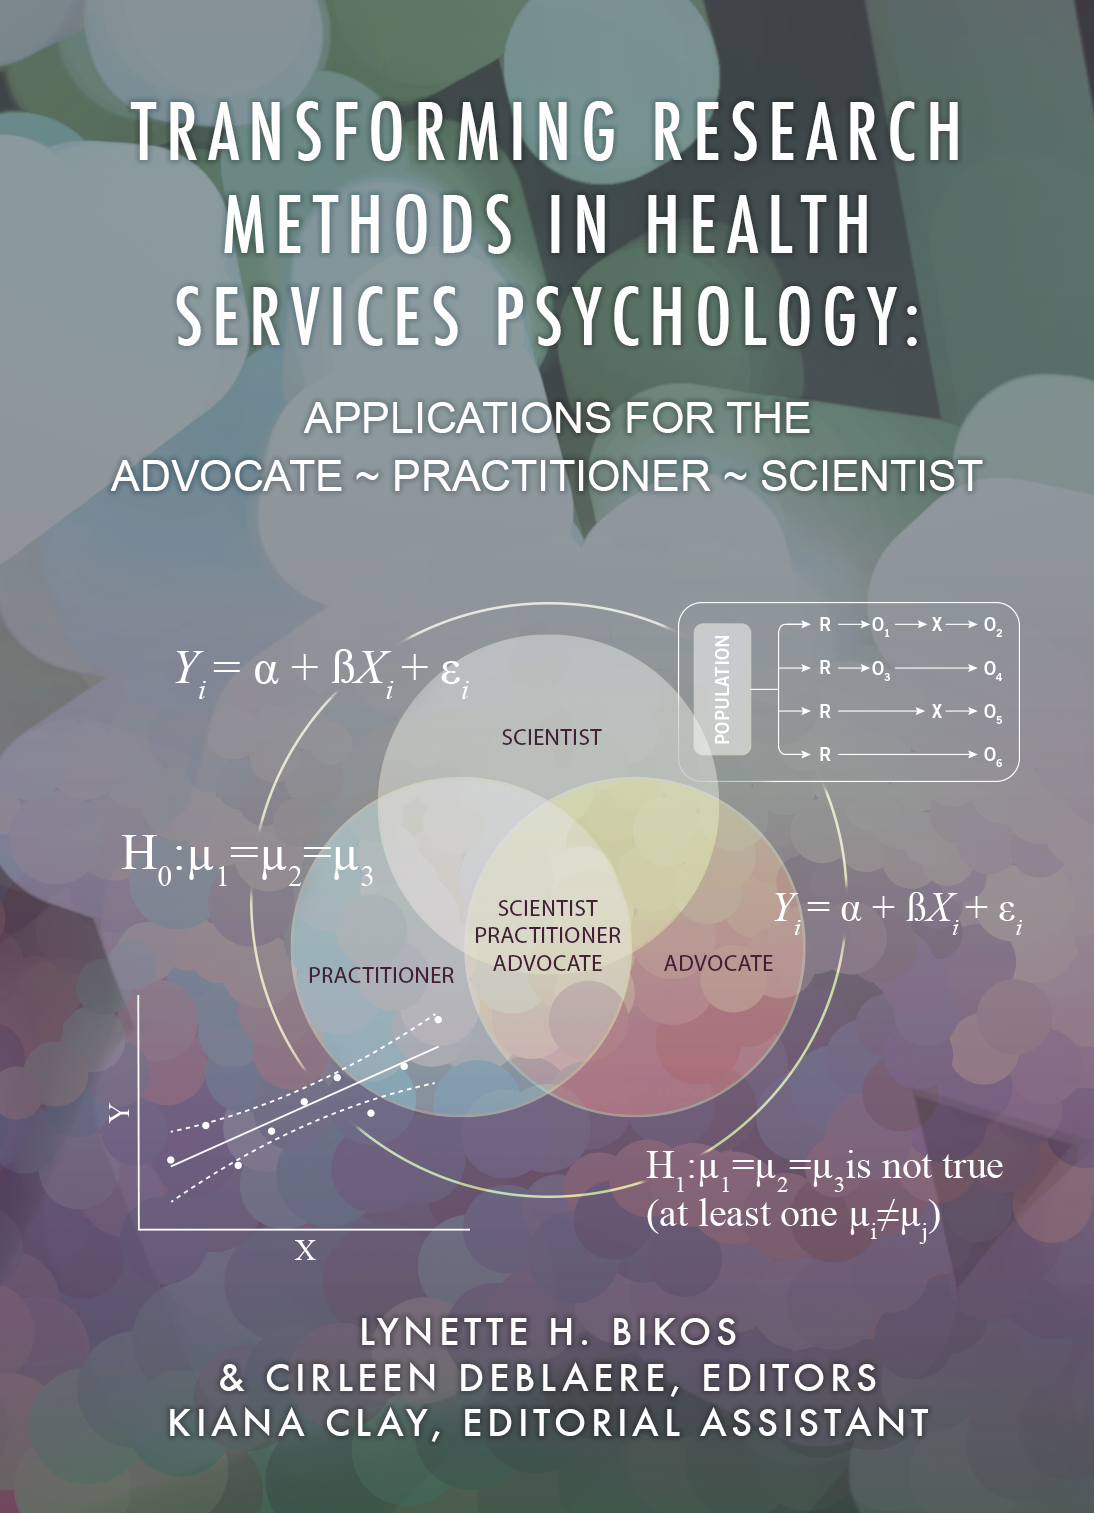
\includegraphics{images/bookcover.png}
\caption{An image of the book cover. It includes three overlapping, pastel-colored, circles representing advocacy, practice, and science. These are surrounded by a handful of statistical symbols and formulae. methods.}
\end{figure}

This open education resource is available in the following formats, all available in the \href{https://github.com/lhbikos/TransformingResearchMethods/tree/main/docs}{docs} folder at the GitHub repository:

\begin{itemize}
\tightlist
\item
  Formatted as an \href{https://lhbikos.github.io/TransformingResearchMethods/}{html book} via GitHub Pages available
\item
  As a \href{https://github.com/lhbikos/TransformingResearchMethods/blob/main/docs/TransformingResearchMethods.pdf}{PDF}
\item
  As an \href{https://github.com/lhbikos/TransformingResearchMethods/blob/main/docs/TransformingResearchMethods.epub}{ebook}
\item
  As a \href{https://github.com/lhbikos/TransformingResearchMethods/blob/main/docs/TransformingResearchMethods.docx}{Word Document}
\end{itemize}

All materials used in creating this OER are available at its \href{https://github.com/lhbikos/TransformingResearchMethods}{GitHub repo}.

\chapter*{PREFACE}\label{preface}


\textbf{If you are viewing this document, you should know that this is a book-in-progress. Early drafts are released for the Transforming Counseling Psychology Curriculum Showcase at APA 2022, for peer review, and for generating interest in collaboration. The document was last updated on 30 Jan 2025}.

In her 2021-2022 term as President of the Society of Counseling Psychology, one of Dr.~Amy Reynolds' Presidential Initiatives was \emph{Transforming Counseling Psychology Curriculum and Praxis.} Dr.~Reynolds invited counseling psychology faculty, practitioners, and doctoral students ``to critically examine and deconstruct how various competencies, courses, and content are taught; how we socialize our students; and then re-imagine, dream, and reconstruct new and transformative ways to teach and train.''

\section*{Strategies for a Social Responsivity}\label{strategies-for-a-social-responsivity}


This open education resource (OER) is a product of the group devoted to \emph{research}. There are a number of strategies we used to ensure that the OER moves in the direction of being socially and culturally responsive.

\begin{itemize}
\tightlist
\item
  Our authors committed to using the guidelines for a liberated syllabus found in the CCTC: Social Responsiveness in \href{https://pr4tb8rrj317wdwt3xlafg2p-wpengine.netdna-ssl.com/wp-content/uploads/2021/05/CCTC_Socially-Responsive-HSP-Ed-Training_v7.pdf}{Health Services Psychology Education \& Training Toolkit}.
\item
  We chose the format of OER because provides a zero-cost \emph{textbook} to faculty and students.
\item
  We sought authors and co-author teams that represent the diversity of health services psychology including discipline (counseling, clinical, educational),stage in career (students, early career professionals, mid- and late- career professionals), and identities that have been marginalized in higher education and our discipline.
\item
  Each chapter works its way through an open peer review process where the chapter (with authors clearly identified)is hosted in a shared drive. At least two reviewers can mark up the same document and contribute to the same rubric. At any time the author(s) can see the review and, if desired, dialogue with the reviewers. At the outset, we specified the tone to be ``formative not summative.''
\item
  Although we are still learning, we have attempted to use tools and techniques that are consistent with universal design. For example, we hope that the image captions and headers are marked such that text readers will identify them as such.
\end{itemize}

\section*{Perpetually in Progress}\label{perpetually-in-progress}


This book is being formatted in R Markdown, rendered into its ``book'' format with Bookdown, hosted on GitHub, and pushed to the internet (in its html format) through GitHub Pages. This set of tools allows the book to be \emph{perpetually-in-progress.} This means that our authors can update their chapters at-any-time. It also means that we can add chapters at-any-time. If you are interested in contributing to the book, please contact us. It is one of our greatest hopes that this flexibility contributes to the socially and culturally responsive pedagogy that we intend.

\section*{Under Construction}\label{under-construction}


At this stage in the OER's development, authors are still writing and revising chapters. The following designations will identify the chapters that have not been through the review process:

\begin{itemize}
\tightlist
\item
  \emph{In-progress} means that the chapter is partially written (or perhaps outlined) and that the author(s) are continuing to work on the chapter.
\item
  \emph{Under review} means that the chapter is being (or has been) peer-reviewed.
\end{itemize}

\section*{Acknowledgements}\label{acknowledgements}


Financial support, supporting the copy editing and desktop publishing for this project was provided by the Office of Education, Technology, \& Media, Seattle Pacific University (Summer 2022).

The book cover was designed by Dominic Williamson, Senior Instructional Designer in Graphics \& Illustrations, in the Office of Education, Technology, \& Media at Seattle Pacific University.

\section*{Copyright with Open Access}\label{copyright-with-open-access}


This book is published under a a Creative Commons Attribution-NonCommercial-ShareAlike 4.0 International License. This means that this book can be reused, remixed, retained, revised and redistributed (including commercially) as long as appropriate credit is given to the authors. If you remix, or modify the original version of this open textbook, you must redistribute all versions of this open textbook under the same license - CC BY-SA.

A \href{https://github.com/lhbikos/TransformingResearchMethods}{GitHub open-source repository} contains all of the text and source code for the book, including data and images.

\chapter{Internal and External Validity in Health Service Psychology}\label{InExVal}

\emph{Franco Dispenza, PhD (he/him/his) \& Alec Prince (he/him), MPA}\\
\emph{Georgia State University}\\
\emph{Georgia State University is located on the traditional homelands of the Muscogee Creek and Cherokee Nations}

The focus of this lesson is to provide a review of internal validity, external validity, threats to validity, and current trends and considerations in relation to validity. Internal and external validity are foundational to experimental and quasi-experimental research. In experimental and quasi-experimental research designs, health service psychologists work thoughtfully and diligently to ensure that a line of systematic inquiry demonstrates some degree of internal and external validity. This is because psychologists and behavioral health researchers are concerned with making reasonable epistemological claims that could directly impact the lives of diverse communities and populations, especially in research studies attempting to show if particular interventions, treatments, or programs have a true effect on specific outcomes.

Whereas researchers utilizing qualitative frameworks may be more interested in methodological integrity (e.g., credibility and transferability; Levitt et al., 2017), researchers employing quantitative-based paradigms are especially interested in internal and external validity. You will notice that the term ``validity'' is used in many concepts and research frameworks, including construct validity, content validity, predictive validity, criterion validity, and statistical conclusion validity. These are all specific types of validity attempting to establish a degree of accuracy or truthfulness in research. Further, the aforementioned forms of validity often have statistical computations and procedures that accompany them (e.g., bivariate correlations, beta weights, etc.). This chapter will not address those forms of validity. Instead, we will focus on internal and external validity, conceptual constructs that rely on methodological procedures and considerations versus statistical calculations.

\section{Learning Objectives}\label{learning-objectives}

Learning objectives for this chapter include the following:

\begin{itemize}
\tightlist
\item
  Explain the dimensional features of internal and external validity in experimental and quasi-experimental research.
\item
  List and discuss threats associated with internal and external validity in experimental and quasi-experimental research.
\item
  Discuss and apply established methods for controlling the various threats associated with internal and external validity in experimental and quasi-experimental research.
\item
  Identify and apply their knowledge of internal validity, external validity, and their associated threats to current trends and issues in psychological research.
\item
  Critique and distinguish the strengths and limitations of internal and external validity when applied to socially responsive research.
\end{itemize}

\section{Recommended Readings}\label{recommended-readings}

The following served as critical references in the development of this chapter. We encourage you to review them.

\begin{itemize}
\tightlist
\item
  Campbell, D. T., \& Stanley, J. C. (1963). Experimental and quasi- experimental designs for research. Chicago, IL: Rand McNally.
\end{itemize}

This classic and foundational text introduces readers to internal validity, external validity, and threats to validity as originally proposed by Campbell and Stanley. It also provides readers with an overview of the various experimental and quasi-experimental methodological designs, and how various methodological designs could be used to minimize threats to validity.

\begin{itemize}
\tightlist
\item
  Ferguson L. (2004). External validity, generalizability, and knowledge utilization. \emph{Journal of Nursing Scholarship, 36}(1), 16-22. \url{https://doi.org/10.1111/j.1547-5069.2004.04006.x}
\end{itemize}

Although aimed for a nursing audience, there is much to be gained from Ferguson's (2004) review of external validity, generalizability, and evidence-based practice. Ferguson reviews much of the major conceptual tenets of external validity, including its threats and control strategies. Ferguson also discusses ways in which researchers and practitioners could enhance external validity of research.

\begin{itemize}
\tightlist
\item
  Schmuckler, M.A.~(2001).What Is Ecological Validity? A Dimensional Analysis. \emph{Infancy, 2}(4), 419-436. \url{https://doi.org/10.1207/S15327078IN0204_02}
\end{itemize}

Schmuckler (2001) introduces readers to a subset of external validity, namely ecological validity. Schmuckler provides an historical review of ecological validity, and a discussion of the various dimensions, advantages, and criticisms of ecological validity.

\section{Internal Validity}\label{internal-validity}

Health service psychologists are committed to accuracy, honesty, and truthfulness when engaging in the research process. Whether representing research findings fairly, capturing the essence of people's lived experiences with precision, or using research to advocate against harmful psychological practices, researchers are compelled to uphold the integrity of the knowledge claims they make through their scholarship. Researchers are committed to ensuring that their research is justifiable, well-grounded, and internally valid.

\emph{Internal validity} is the extent to which a researcher can infer cause-effect relationships between a set of variables, while simultaneously excluding the influence of confounding or extraneous variables (Campbell \& Stanley, 1963; Cook \& Campbell, 1979). In an attempt to establish internal validity, it is important to rule out the effects of confounding or extraneous variables. \emph{Confounding or extraneous variables} can serve as potential rivals to inferred relationships, leading a researcher to be less confident about the conclusions and implications that can be made between an independent (or treatment) variable and a dependent (or outcome) variable.

\emph{Methodological control} is also paramount in experimental and quasi-experimental research. In an ideal research scenario, a researcher will have identified and controlled for all possible confounds and extraneous variables that may be inherent in the methodological design of a study. Since determining causality is the goal in experimental and quasi-experimental research, such a scenario would render a study to be high in internal validity. However, we know in practice there is no such thing as a perfect study, especially when there exist numerous \emph{threats to internal validity}. Threats consist of factors or conditions that endanger a researcher's capacity to amplify a study's level of internal validity (Onwuegbuzie \& McLean, 2003).

\subsection{Threats to Internal Validity}\label{threats-to-internal-validity}

Researchers often execute considerable forethought when identifying and eliminating potential threats to internal validity. Psychological researchers are encouraged to use a variety of logic-informed heuristics, ``what if'' sensitivity analyses, or consider any new data or findings to rule out rival hypotheses (Kenny, 2019). Researchers are also encouraged to consider more classically identified threats to their research design (Campbell \& Stanley, 1963). Some of the most common threats to internal validity consist of history, maturation, instrumentation, statistical regression, selection, attrition, and experimenter bias (Campbell \& Stanley, 1963; Cook \& Campbell, 1979; Shadish et al., 2002). Threats to internal validity can occur, or be discovered, at any point during the research process, including design, implementation, data collection, and analyses. There can exist multiple threats in a given study, and these threats can also intersect with one another. Keep in mind that threats are never something a researcher just ``checks off'' in a box, but rather a researcher continuously monitors their methods to ensure the credibility of the concluded findings (Onwuegbuzie \& McLean, 2003). Each threat to internal validity is discussed in more detail below.

\subsubsection{History}\label{history}

No researcher can control the potential of geological, sociopolitical, financial, cultural, climate-related, pandemic, and other national and global events from impacting individuals in a research study. But inevitably such events happen, and unfortunately with what seems to be at higher frequencies these days. Historical events can influence the manner in which participants respond to a study's dependent variable, making it difficult for researchers to determine whether an observed outcome was the result of a study's independent variable or the historical event. In some instances, the historical event could directly intersect with objectives of the study itself making it even more difficult for researchers to make valid conclusions. Imagine you are evaluating the effectiveness of a new stress-reduction intervention for survivors of catastrophic hurricanes in a low-income, rural community in the southeast United States. In the middle of implementing the intervention, a tornado hits the same community, leading to severe damage and loss of life. What impact will this historical event have on the research study?

\subsubsection{Maturation}\label{maturation}

Development and growth are natural processes that occur for individuals during their lifespan. These processes could be physiological, cognitive, social, or emotional. Given the length of a particular study, sometimes results from a study may be more indicative of naturally occurring growth and developmental factors, versus any manipulated independent variable.

\subsubsection{Instrumentation}\label{instrumentation}

No tool, test, or measure used in research can be entirely valid and reliable one hundred percent of the time. Instruments can produce low reliability scores or even produce inadequate psychometric properties (e.g., construct and predictive validity) with a study's particular sample. This is an important consideration as some tests and measures were never validated or normed with diverse samples. Consider a measure of marital satisfaction that was created using heterosexual couples in the Netherlands. The measure may have great face validity, and even demonstrate adequate levels of content, criterion, and construct validity. But it may not produce the same psychometrics if used in married couples in the United States. It may be entirely inappropriate to use this measure if the United States sample also includes same-sex couples. Lastly, human beings administering instruments could contribute additional error, making instrumentation a serious threat to research studies. For example, some researchers may become fatigued when administering some measures, may not be consistent with measurement, or may not accurately observe a phenomenon during a research study.

\subsubsection{Testing}\label{testing}

It is common to test participants multiple times throughout the course of a research study. Researchers often use the same test, measure, scale, or inventory when testing participants, but it begs the question as to whether changes in a test---that had been given multiple times---reflect true change? Sometimes referred to either as a \emph{practice effect} or \emph{fatigue effect}, changes in scores on the same test may be the result of familiarity with the test or becoming tired with the test.

\subsubsection{Statistical Regression, or Regression to the Mean}\label{statistical-regression-or-regression-to-the-mean}

Sometimes researchers select participants based on high or low scores on a particular test or measure (Campbell \& Kenny, 1999). For example, researchers may be interested in examining people who score high on measures of academic or cognitive functioning. If retested, those same participants may continue to score high or low. However, not all would score as high or low because of statistical regression, or regression to the mean. When participants are retested, researchers find that scores are less extreme and center toward an average score. Imagine a researcher was interested in testing a career counseling intervention with first generation college students who reported high scores on career indecision and anxiety in a career battery of questionnaires. After the intervention is complete, the researchers issue a final battery of questionnaires. These same first generation college students may appear less anxious and indecisive due to statistical regression to the mean and not necessarily the intervention.

\subsubsection{Attrition, or Differential Mortality}\label{attrition-or-differential-mortality}

Ethically, participants have the right to withdraw from participating in a research study at any given time during the research process. When participants withdraw, or drop from a study, researchers refer to this as attrition. A major concern of attrition is that it leads to potential biases in scores between groups (or observations in the case of longitudinal studies) that may not reflect whether an independent variable had any effect on the dependent variable. If there is substantial attrition in one group, or across the entire study, it leads a researcher to question why participants are withdrawing. Researchers may further wonder if participants dropping from the study are characteristically different from those who are remaining in the study. Attrition limits the type of conclusions that can be made because observations made across time or between groups may not reflect true differences as a function of the independent variable. Rather, there may be some other underlying issue with the research study.

Imagine a researcher has been evaluating the effects of a six-session mindfulness cognitive behavioral group intervention for the reduction of race related stress among Black and African American women employed in a large healthcare setting. The researcher used a longitudinal, between group experimental design with an intervention group (treatment) and a control group (education), but found that attrition rates were higher for those in the control than for the intervention group. Equivalent and adequate comparisons could not be reliably made between the two groups at completion of study, so the researcher decided to send surveys to those dropped from the study and inquire why they dropped. The surveys return and the researcher finds that a significant portion of the control group were made up of on-call, ambulatory nurses who were unable to commit to the scheduled sessions. Therefore, the attrition was the result of some characteristic that differentiated the two groups.

\subsubsection{Experimenter Bias}\label{experimenter-bias}

Researchers need to ensure they do not engage in verbal or nonverbal behaviors that inadvertently alter the results of a study. Sometimes this is referred to as an \emph{experimenter expectancy}, and it is even known as the \emph{Rosenthal Effect}. This becomes a threat when a participant's response in a study is the result of the experimenter's expectations versus the manipulated or independent variable. Examples include emphasizing particular words when reading prompts or scripts, or excessive nodding and smiling when certain favorable responses are solicited by study participants.

\subsubsection{Selection Bias}\label{selection-bias}

Differences between groups in experimental studies can sometimes be the result of characteristics of the participants themselves, versus the manipulated or independent variable. For instance, a researcher may have accidentally grouped people along the same characteristic, such as sex, gender, sexual orientation, race, ethnicity, or age group. This potentially sets up nonequivalent groups in experimental or quasi-experimental research, and makes it difficult for researchers to determine whether any changes in dependent or outcome variables were the result of an independent variable or the characteristic itself. This also pertains to self-selection bias commonly seen in survey and questionnaire research, in which participants self-select to participate in a study.

\subsection{Controlling for Threats to Internal Validity}\label{controlling-for-threats-to-internal-validity}

Researchers have identified a number of methodological procedures that could be used to control for threats to internal validity (Campbell \& Stanley, 1963; Cook \& Campbell, 1979; Fabrigar et al., 2020; Onwuegbuzie \& McLean, 2003; Shadish et al., 2002). Below we discuss the importance of considering control groups, random assignment, matching, blocking and holding variables constant.

\subsubsection{Control Groups}\label{control-groups}

Control groups are commonly used in experimental and quasi-experimental human subjects research, and there is an important logic to its use. Individuals are assigned to a group (or condition) in which they do not receive the treatment or manipulated variable. However, participants do partake in similar tasks and conditions (e.g., complete surveys, questionnaires, physiological markers, etc.) as those in the experimental condition. Upon completion of the study, researchers then compare how the intervention or experimental condition performed alongside the control condition or group. Control groups are particularly effective at controlling for the effects of history, maturation, testing, instrumentation, and regression toward the mean (Campbell \& Stanley, 1963; Cook \& Campbell, 1979).

\subsubsection{Random Assignment}\label{random-assignment}

Considered one of the most robust methods to control against threats to internal validity, researchers randomly place volunteer participants in various study conditions at the very beginning of a research study. This assures the researcher that each participant had the same or equally probable chance of being placed in either an experimental condition (or group) or a control condition (or group), while helping to decrease any unknown or intentional influence on assignment of participants to different groups. It further assures the researcher that the groups are equitable in terms of various characteristics of the participants (e.g., demographics, temperament, etc.; Fabrigar et al., 2020). Any observed differences or changes seen among the groups or conditions could then be accounted for by the manipulated independent variable or the applied intervention. More importantly, any observed difference between the groups is not the result of any sort of systematic bias that might have occurred during the initial phases of the research study.

Take a hypothetical scenario in which a researcher is evaluating the ways in which implicit sexist messaging influences women's responses to a cognitive motor task. Women are recruited from the community to participate in the study. One group receives the implicit sexist messaging while the other group does not. However, nearly all members in one group happened to be women between the ages of 21 and 29, while the majority of those in another group were women between the age of 43 and 56 This could constitute a systematic bias since there are generational differences between members in one group versus the other. Random assignment is incredibly important when controlling for the effects of selection (Campbell \& Stanley, 1963; Cook \& Campbell, 1979; Shadish et al., 2002).

It is important to keep in mind that random assignment and random sampling are not synonymous with one another. \textbf{Random sampling} is when researchers utilize a variety of probable sampling techniques (e.g., simple, systematic, stratified, or cluster) to recruit participants who approximate the general population. It also means that all members of a given population have an equal chance of being recruited to participate.

\subsubsection{Matching}\label{matching}

To further avoid the threat of selection bias, researchers may engage in the process of participant matching. This is especially helpful if a researcher cannot guarantee equivalent groups through randomization, or when sample size may be too small. Participants are matched on a variety of characteristics (e.g., cognitive or intelligence pre-test scores, gender, age, etc.), by placing members of similar characteristics in either an experimental/intervention condition or in the control condition. This helps a researcher establish some degree of equivalence between groups within a particular sample.

\subsubsection{Blocking and Holding Variables Constant}\label{blocking-and-holding-variables-constant}

Researchers may also choose to use some characteristic in the study's sample (e.g., cognitive or intelligence scores, ethnicity or race) as an additional independent variable. This is referred to as \emph{blocking}. Unlike matching, researchers may employ this strategy to see if a particular characteristic of the sample has an effect on the dependent variable. Alternatively, some researchers may choose to hold a particular characteristic constant or homogenize some sample characteristic so as to eliminate any undue influence from extraneous characteristics of a sample. For instance, a researcher may choose to only recruit high school aged adolescent boys between the ages of 14 and 15 who score above a certain threshold on an anxiety and depression measure to participate in a short-term emotional regulation treatment study.

\section{External Validity}\label{external-validity}

Many researchers invest time and resources with the hopes of expanding their research findings to larger communities and contexts, especially if the research is aimed at alleviating any suffering or influence larger systemic change efforts. Thus, researchers are not only concerned with internal validity, but also the external validity of their study. \textbf{External validity} is the degree towhich research findings can be generalized to the population that approximate the original context of the study (Campbell \& Stanley, 1963; Cook \& Campbell, 1979; Shadish et al., 2002).

External validity is also concerned with the degree in which a study can be generalized across broader populations, treatments, settings, and conditions (Ferguson, 2004). Researchers wish to move beyond the controlled setting in which the study originally took place, and further consider ways that the findings may apply in other diverse applicational settings, time, persons, or slightly different variables or targets (Kenny, 2019; Shadish et al., 2002). For instance, a researcher who evaluated the effectiveness of a minority stress reduction intervention for transgender and gender nonbinary individuals in a controlled laboratory setting at a university, might have interest in seeing the intervention applied or replicated with transgender and gender nonbinary individuals in community based clinics, private practices, college counseling centers, and other agencies across the United States. That same researcher may have further interest in having their research used to inform policy on affirming psychological care for transgender and gender nonbinary individuals for all mental health practitioners.

Researchers always have the hope that the finding of their research will have some degree of relevance and importance in ``real-world'' settings, particularly if study findings are replicated in other contexts. Replicated studies that support original study findings are considered to demonstrate high levels of external validity, as well as other forms of validity (e.g., internal validity, construct validity; Fabrigar et al., 2020). As a variation, or subcategory of external validity, \textbf{ecological validity} is concerned with whether a study's results can be applied to naturalistic or representative settings in every-day life (Andrade, 2018; Schmuckler, 2001). With this in mind, it is important to consider that there also exist threats that could interfere with a researcher's confidence in the external validity of their study's findings.

\subsection{Threats to External Validity}\label{threats-to-external-validity}

Campbell and Stanley (1963) identified four particular threats, including reactive or interaction effects of testing, interaction effects of selection bias, reactive effects of arrangement, and multiple treatment interference.

\subsubsection{Reactive or Interaction Effect of Testing}\label{reactive-or-interaction-effect-of-testing}

Sometimes researchers need to be cognizant that research studies, experiments, and testing procedures---in and of themselves---may be the catalyst producing some of the findings we see from research. In many ``real-world'' conditions, people are not tested or observed as much as they are in research. In particular, Campbell and Stanley (1963) discussed how exposure to a pre-test condition, or multiple testing conditions, may influence a study participant's degree of sensitivity to the experimental variable. Consider an example in which a researcher is interested in examining a clinical supervisor's attitudes toward racial and ethnic microaggressions in counseling. The clinical supervisor is asked to view a fictitious counseling session of a supervisee, and then asked to identify any subtle instances of discrimination from a 10 minute clip of a counseling session. Afterwards, the researcher follows up with another post-test to see if there have been any changes in attitudes toward racial and ethnic microaggressions in counseling. The potential threat to external validity in this example is that the clinical supervisors in the study have been sensitized by the pre-test condition (i.e., the fictitious counseling session), increasing their potential chances of identifying microaggressions in a counseling session. If generalized out, clinical supervisors may not respond the same way since they've not been pre-tested and sensitized.

\subsubsection{Interaction Effects of Selection Bias}\label{interaction-effects-of-selection-bias}

Health service psychologists pay close attention to samples, and work diligently to recruit adequate samples to participate. However, there are situations in which a particular sample in a research study would not generalize to the entire population. This could be the result of selection bias. For instance, many university researchers utilize an undergraduate psychology research pool to recruit participants for their research. But undergraduate students represent a biased sample, and do not reflect the larger population in terms of representative demographics. Thus, researchers replicating a study with a different sample may not obtain the same findings.

\subsubsection{Reactive Effects of Experimental Arrangements}\label{reactive-effects-of-experimental-arrangements}

Research conducted in highly controlled settings (e.g., sterile laboratories) run the risk of not generalizing well in ``real world'' diverse settings or populations. This is mainly to do with the fact that research participants are willing volunteers who understand they are fully participating in experimental or study-related activities. In some instances, research participants may respond or behave a certain way because they are being observed. Frey (2018) reports that a participant may even have the desire to please a researcher by altering their performance on a particular outcome. This may sound familiar because you may understand this to be the \textbf{Hawthorne effect}, a phenomenon in which human beings change their behavior as a result of being observed.

\subsubsection{Multiple Treatment Interference}\label{multiple-treatment-interference}

Depending on the sequencing of a particular study, researchers may provide the same subject different treatments or interventions at different intervals. For example, a researcher may be testing multiple formats to examine the combination of psychotropic medication along with some type of psychotherapy. However, this makes it difficult for researchers to determine if the sequencing of the differing treatments played any role in any of the observed outcomes. Because of this type of sequencing, we would argue that there has been some level of treatment contamination, because it is difficult to control effects from previous treatments or studies.

\subsection{Controlling for Threats to External Validity}\label{controlling-for-threats-to-external-validity}

It is important to note that external validity can never be assured, even when a researcher stringently addresses and controls for threats to internal validity (Ferguson, 2004). However, there are some threats to external validity that can be managed through some methodological considerations. Below we discuss only a few, including random selection, concealed research, as well as counterbalancing and strategies to control for pre-testing effects. \#\#\#\# Random Selection Sometimes confused with random assignment (already discussed above as a means of controlling threats to internal validity), random selection is about accessing and including a representative sample of the target population in a research study. Random sampling procedures, such as simple or stratified sampling, play a significant role when it comes to random selection. You may recall that random sampling is concerned with the notion that every individual (or observation) has an equal probability of being selected for a study. The equal probability of being selected then increases the probable chances that research findings can be generalized back to the target population (Ferguson, 2004). This form of control is particularly beneficial when considering the interaction effects of selection bias.

\subsubsection{Single, Double, and Triple-Concealed Research}\label{single-double-and-triple-concealed-research}

It is important to preface that the term often used in research texts is single, double, and triple ``blind'' research. However, we believe ``blind'' is often misused in a variety of contexts, and in this context we believe it perpetuates ableist ideologies. And so, we offer a slight modification by using the term ``concealed.'' In order to reduce overt and covert forms of researcher bias in a study, researchers attempt to conceal as much as possible from participants and other members of a research team. In a single-concealed research study, only the researcher knows if participants are in a control or experimental group. Participants do not know what condition they are in. In a double-concealed research study, neither the researcher or participant know which is the control or experimental group. In a triple-concealed research study, consistent with the double-concealed design, neither the researcher nor participant know if they are in the control or experimental group. Additionally, those responsible for analyzing or examining outcomes do not know which set of variables were the control or experimental condition. This form of control is especially helpful when addressing reactive effects of experimental arrangements.

\subsubsection{Counterbalancing and Controlling for Pre-Test Effects}\label{counterbalancing-and-controlling-for-pre-test-effects}

In order to address the effects of multiple treatment interference, or carryover effects, a researcher may consider the use of counterbalancing. A researcher must decide \emph{a priori} all the possible sequences for a treatment, implement those varying permutations, and evaluate study participants in those different orders in order minimize carryover effects. If pre-testing effects is a concern, a researcher may decide not to include a pre-test at all, and compare groups at post-test only. Relatedly, a researcher may want to consider the use of the \emph{Solomon Four-Group Design} as a means of countering the effects of a pre-test (Allen, 2017). In a Solomon Four-Group Design, a researcher will have four groups, in which some groups receive a pre-test and other groups do not.

\section{Current Issues, Trends, and Considerations}\label{current-issues-trends-and-considerations}

We will briefly review current issues, trends, and consideration of internal and external validity. It is vital that health service psychology researchers attend to matters of multiculturalism and diversity, since this has direct implications on the external and ecological validity of study findings. It is also incredibly important to consider evidence based practices with culturally diverse populations. Replication of research is another pressing trend in the field of psychology that requires researchers to consider how they present and disseminate their research findings to broader communities. Relatedly, Internet-based collection procedures require new concerted efforts in our conceptualization of internal control and generalizability of results. We end with a recommendation that researchers could consider when addressing internal and external validity of research.

\subsection{Validity Issues Related to Cultural Diversity}\label{validity-issues-related-to-cultural-diversity}

In a critique of psychological research, Sue (1999) wrote that researchers have overemphasized internal validity over external validity. As a result, the overemphasis on internal validity has hindered the development of research on ethnic and racial minority groups, as well as other marginalized groups. Unfortunately, this has further perpetuated psychology's own history of reinforcing oppression and inequality (Lewis, 2021). This has also led to a tension between ``basic'' researchers who privilege statistical power and high degrees of internal validity and ``applied'' researchers who privilege the nuance of intersectional research and external or ecological validity (Lewis, 2021).

As an issue of validity, psychological based research has often failed to include diverse participants, or it has failed to report on the diverse identities within samples. A 36-year review of randomized clinical trials of depression (from 1981-2016) found that less than half of the studies reported on the sample's race/ethnicity, about one in six trials had a predominantly ethnic minority sample, and one in seven studies had a predominantly low socioeconomic (SES) sample (Polo et al., 2019). Similarly, researchers have found inconsistency in demographic data collection and reporting. Racial and ethnic minority groups are often underrepresented, along with disability, and diverse sexual orientations (Greenwell \& Hough, 2008). Within research on the lesbian, gay, bisexual, transgender, queer (LGBTQ+) communities, the needs of cisgender white gay men have been privileged, and the experiences of LGBTQ+ individuals who represent women, people of color, transgender, or bisexual communities have largely been omitted or excessively medicalized (American Psychological Association, 2015; American Psychological Association, 2021; Hegarty \& Rutherford, 2019).

Researchers have noted the importance of consistently collecting and reporting demographic data on race, ethnicity, sexual orientation, gender identity, SES, disability, and other identities (dickey, Hendricks, \& Bockting, 2016; Greenwell \& Hough, 2008; Polo et al., 2019). For instance, dickey and colleagues (2016) stressed the importance of collecting and analyzing gender identity and sexual orientation data separately in population surveys, especially since gender identity is often conflated with sexual orientation. Parent and colleagues (2013) encourage researchers to focus on the context of intersecting oppressions in addition to intersecting identities, to ensure that diverse populations are included in psychological research.

To redress the exclusion of marginalized identities from psychological research and scholarship, researchers recommend going beyond including marginalized individuals in samples to including them in creating the studies themselves. Participatory research is an umbrella term for research that engages those being studied in the production of knowledge to promote education and change (Cargo \& Mercer, 2008). Participatory research in its many forms has been implemented with gender and sexual minority populations, refugees, individuals with disabilities, and racial and ethnic minority communities around the globe (Cargo \& Mercer, 2008; Fine et al., 2021; Jacquez et al., 2021). Fine et al.~(2021) argue that ``the move to include and privilege those most impacted by injustice as co-researchers is not simply an act of empathy or decolonizing; it is a commitment to good science'' (p.346).

\subsection{Validity Issues Related to Replication Studies}\label{validity-issues-related-to-replication-studies}

In recent years, psychologists have argued that the discipline of psychology suffers from a replication crisis (Fabrigar et al., 2020). This calls into question the validity of psychological research and the findings that have been reported over the years. Some notable cases of outright fraud, questionable research practices (Pashler \& Wagenmakers, 2012), flawed methodologies, and incorrect analysis of data (Fabrigar et al., 2020) have led to some of these replication issues. Others have argued that failures to replicate result from small sample sizes, subsequent low statistical power (Maxwell, Lau, \& Howard, 2015; Schmidt \& Oh, 2016), as well poor statistical conclusion validity (Fabrigar et al., 2020). Schmidt and Oh (2016) argue that ``the real problem is not a lack of replication; it is the distortion of our research literatures caused by publication bias and questionable research practices'' (p.32).

Addressing the replication crisis is no easy task as it requires addressing journal review processes, research practices, and reward structures in academia (Pashler \& Wagenmakers, 2012). The Reproducibility Project, created by the Open Science Collaboration, aimed to address the replication crisis by replicating 100 experimental and correlational studies from key psychology journals (Open Science Collaboration, 2015). The Reproducibility Project found that while 97\% of all the original studies had significant results, only 36\% of replicated studies demonstrated significant results (Open Science Collaboration, 2015). Schmidt and Oh (2016) note the importance of replicating studies with nonsignificant results and recommend meta-analysis as a solution to this issue, provided publishing bias and questionable research practices are addressed.

Some researchers argue that simply replicating studies is not enough to safeguard the validity of psychological research. In an analysis of the Reproducibility Project, Sabik and colleagues (2021) found that the studies reproduced by the Project seldom considered context and identity, even when it was central to the study's design, and that study samples were predominantly WEIRD (people from Western, educated, industrialized, rich, and democratic countries). Further, intersectionality, power, discrimination, and historical contexts were rarely considered in the Project's reports (Sabik et al., 2021). Sabik and colleagues argued that the Reproducibility Project and the discourse surrounding the replication crisis are more concerned with data transparency and methods than with the inclusion of historically oppressed and marginalized groups. To truly move the discipline forward, some argue it is necessary to set aside the emphasis on traditional research methods and reproducibility in favor of methods that center on the co-creation of knowledge (Grzanka \& Cole, 2021).

\subsection{Internet Research and the use of Crowdsourcing Platforms}\label{internet-research-and-the-use-of-crowdsourcing-platforms}

Many social science researchers utilize the Internet (e.g., social media, list servs, emails) for purposes of recruitment and data collection (e.g., Survey Monkey, Qualtrics, etc.). Although this has considerable implications for internal and external validity that go beyond the scope of this chapter, it is essential that we discuss some of the implications of crowdsourcing platforms. Crowdsourcing platforms are online websites that can be used by researchers to recruit potential participants who have access to Internet and an electronic device (Peer et al., 2017). And although we cannot review all of the available crowdsourcing platforms, researchers have several platforms to choose from, including CrowdFlower and Prolific Academic (see Peer et al., 2017 for a review of the various strengths and limitations of these crowdsourcing platforms). However, Amazon's Mechanical Turk (MTurk) has garnered some of the most attention in recent years by methodologists and scholars. It is likely that many of the issues surrounding internal and external validity with MTurk are also applicable to other crowdsourcing platforms, but we will focus mostly on MTurk for this chapter.

Created in 2005 by Amazon, MTurk is an online marketplace where workers (Turkers) complete Human Intelligence Tasks (HITs) for MTurk requesters for pay. This is equivalent to a psychology undergraduate pool, but using a larger sample of the population. Typical HITs are transcribing movies, copying text from images, and participating in surveys. In addition to regular MTurk workers, there are MTurk ``masters'' whose accuracy are validated by previous MTurk requesters. MTurk is used extensively by businesses, academic researchers, and nonprofits (Pew Research Center, 2016). A review of key journals in psychology, psychiatry, and other social sciences found that fewer than 50 studies using MTurk data were published in 2011; in 2015, over 500 studies using MTurk data were published (Chandler \& Shapiro, 2016).

Although MTurk is a cost-effective, efficient method to collect large amounts of data, there are concerns about the reliability and validity of MTurk data. For instance, several researchers have called the external validity of MTurk data into question. Turkers are relatively young and well-educated compared to national averages (Hitlin, 2016; Walters et al., 2018). Walters et al.~(2018) found that MTurk workers' health status and behaviors were not comparable to a nationally representative sample. Compared to a national sample, MTurk users were over twice as likely to screen positive for depression, but they were less likely to exercise, smoke, have asthma, or have health insurance (Walters et al., 2018). Another concern regarding MTurk data is the overall decrease in data quality resulting from an influx of computer programs or ``bots'' that complete HITs and individual users bypassing location restrictions using server farms (``farmers''). Chmielewski and Kucker (2019) conducted the same study over four years and found a substantial increase in low-quality data from MTurkers, including failures to replicate well-established findings, decreases in the reliability and validity of the Big Five Inventory, a widely used personality measure, and increases in participants failing response validity indicators (Chmielewski \& Kucker, 2019).

MTurk remains a valuable resource for collecting data, provided the necessary steps are taken to ensure data quality. Buhrmester et al.~(2018) recommend that researchers take the time to work on MTurk themselves to understand the Turker experience. Other recommendations include screening responses before approving HITs, including validity indicators, and comprehensive reporting on screening and study designs (Buhrmester et al., 2018; Cheung et al., 2017; Chmielewski \& Kucker, 2019; Mason \& Suri, 2011). MTurk is particularly useful for researching hard-to-reach populations such as individuals with disabilities, LGBTQ+ individuals, and those with low socioeconomic status (Smith et al., 2015). To safeguard against Turkers lying about being part of the target group, Smith et al.~(2015) recommend providing monetary incentives that are not overly attractive and asking participants to self-identify prior to sharing the purpose of the research. Walters at al.~(2018) suggested that researchers would benefit from using MTurk workers over masters because the two groups were comparable in demographics and health characteristics; however, workers are a larger sample and more cost-effective. With adequate measures to ensure data quality, MTurk remains an efficient and cost-effective option for researchers, especially those studying hard-to-reach populations.

\section{A Consideration for Practice}\label{a-consideration-for-practice}

First introduced in 1999, the RE-AIM framework is a tool that can help researchers balance internal and external validity when planning, designing, and evaluating health-related interventions (Dzewaltowski et al., 2004). Originally intended as guidelines for reporting research results, the framework is now also used to organize literature reviews and to translate research into practice. This has incredible implications for both internal and external validity, as it attempts to take a study beyond just epistemology and into direct practice with populations.

The RE-AIM framework's five dimensions include: \emph{Reach, Efficacy/Effectiveness, Adoption, Implementation, and Maintenance} (Dzewaltowski et al., 2004; Glasgow, Vogt, \& Boles, 1999). Reach and Efficacy/Effectiveness are both individual-level dimensions. Reach considers the percentage of the population of interest included in the intervention and how representative they are, whereas Efficacy/Effectiveness considers the impacts (both positive and negative) on participants (Dzewaltowski et al., 2004; Glasgow, Vogt, \& Boles, 1999). Adoption and Implementation are organizational-level dimensions that consider the type and proportions of settings that will adopt the intervention and the extent to which the intervention is implemented faithfully in the real world (Dzewaltowski et al., 2004; Glasgow, Vogt, \& Boles, 1999). Finally, Maintenance examines the continuity of the program over time at both the individual and the organizational levels (Glasgow, Vogt, \& Boles, 1999).

RE-AIM is used in a variety of fields and settings, such as chronic illness management, mental health, smoking cessation, health policy, and diabetes prevention (Kwan et al., 2019). Although the RE-AIM framework is becoming more widely used, a systematic review noted that the framework is often used inconsistently (Gaglio, Shoup, \& Glasgow, 2013; Glasgow et al., 2019). Several adaptations and clarifications have been offered to mitigate confusion and inconsistency using the RE-AIM framework. Holtrop and colleagues (2018) offered guidance on integrating qualitative methods into the RE-AIM framework. Holtrop et al.~(2021) offered clarifications on common misconceptions about the framework. The Practical, Robust, Implementation, and Sustainability (PRISM) model is an emerging complement to the RE-AIM framework that focuses on contextual factors (Glasgow et al., 2019). With the original goals of producing valid and relevant research and translating research into practice, RE-AIM and PRISM will continue to grow and evolve as researchers apply these frameworks to new populations and settings. Researchers and students can directly go to the website to learn more about how to implement these principles in their research, as well as access various resources, tools, and checklists (\url{http://www.re-aim.org}).

\section{Activity}\label{activity}

Take a moment to locate the latest issue of a peer-refereed journal in your respective field. Some example psychology journals published by the American Psychological Association include the \emph{Journal of Counseling Psychology, School Psychology, Journal of Consulting and Clinical Psychology, Health Psychology, Developmental Psychology, or Professional Psychology: Research and Practice}. Once you have located a recent issue, browse through the table of contents and select a quantitative article that may be of interest to you. Read the article and then consider the following prompts:

\begin{enumerate}
\def\labelenumi{\arabic{enumi}.}
\tightlist
\item
  Which threats of internal validity were identified and controlled for in the study? Were any explicitly identified and addressed by the authors the article? Were there any that you noticed that were not addressed or controlled for in the study?
\item
  How were study participants recruited or sampled for the study? In what ways were study participants diverse?
\item
  What limitations were mentioned in the discussion section? Were issues of internal and external validity explicitly named? If so, which ones? If not, which internal and external validity issues were implied?
\item
  How would you replicate the study you read? What additional validity factors would you consider to improve the new proposed study's internal and external validity?
\end{enumerate}

\section{References}\label{references}

\chapter{Understanding Training Models and the Factors that Transcend Them}\label{TrainMod}

\emph{Rachel M. Chickerella (she/her) PhD, Antioch University New England}\\
\emph{Karen Meteyer (she/her), PhD, Antioch University New England}\\

\emph{Antioch University New England is located on the traditional homelands of N'dakinna, the ancestral homeland of the Abenaki people along the Kwanitekw (Connecticut) and Ashuelot watersheds.}~

Research methods are the tools used by psychologists and others to collect and analyze data to understand new information or further understand a topic (University of Newcastle Libguides, 2023). Psychologists may employ a range of research designs including quantitative approaches that use numbers to capture information about variables and qualitative designs in which phenomena are represented with words. Though competency in research methods is considered essential to becoming a professional psychologist, or a psychologist engages in clinical work (Rutgers University Catalogs, 2023), there are different approaches to imparting the skills and knowledge to students which reflect distinct training models. Although each degree program in psychology will offer its own unique identity in how it trains students, there are commonalities among models of training. The emphasis placed on certain types of research (qualitative vs.~quantitative), the specific techniques that are taught (e.g., statistics) and the level of proficiency expected of students will all vary as a function of the training model. Understanding the different training models and how they approach teaching research methods will help students select the type of degree and program that will best prepare them to achieve their career goals.

\section{Learning Objectives}\label{learning-objectives-1}

Learning objectives for this chapter include the following:

\begin{itemize}
\tightlist
\item
  Define training models in professional psychology for programs and professors.
\item
  Identify the value of research and quantitative/ qualitative literacy as a competency for programs and professors.
\item
  Explore ways for professors and programs to integrate social justice regardless of training model.
\item
  Describe the importance of qualitative literacy along with quantitative literacy for professional psychology programs and professors.
\item
  List ways to motivate students to engage in course content despite an often perceived boredom related to research methods content.
\end{itemize}

\section{Recommended Readings and Resources}\label{recommended-readings-and-resources}

The following are three works to consider.

\begin{itemize}
\tightlist
\item
  American Psychological Association. (2012). A practical guidebook for the competency benchmarks. Washington DC: APA.
\item
  DeAngelis, T. (2003). Three Programs: Three Different Training Models. American Psychological Association. \url{https://www.apa.org/gradpsych/2003/09/three-programs}
\item
  Okun, T. (2021). White supremacy culture--Still here. Dismantling Racism. Dismantalingracism.org
\end{itemize}

\section{Training in Professional Psychology: An Overview}\label{training-in-professional-psychology-an-overview}

In pursuing a degree in psychology, there are a multitude of paths students may take. A prospective student may first decide if they are going to pursue a professional psychology degree or a non-professional degree. Pursuing a professional degree means that following the degree and licensure, the individual would be eligible to practice as a psychologist. Health service psychology is another term used to describe programs that use a competency based model to promote the development of practicing psychologists \citep{noauthor_what_nodate}. Some pursuits of psychology do not fall under the professional psychology realm, including social, cognitive and experimental psychology. These degrees focus more on research and teaching pursuits. Professional psychology includes multiple disciplines including counseling, clinical and school psychology \citep{noauthor_types_nodate}.

Clinical psychology programs tend to be housed within the psychology department of educational institutions. Students in these programs typically receive training in understanding and diagnosing pathology \citep{noauthor_counseling_nodate}. Clinical psychology is the most common degree conferred \citep{noauthor_types_nodate}. Counseling psychology is another form of professional psychology. Counseling Psychology programs may be housed in the psychology department, but may also be placed in the education department \citep{noauthor_types_nodate}. Counseling psychologists tend to put less emphasis on psychopathology and more focus on treating the whole person \citep{noauthor_counseling_nodate}. Finally, School psychologists may be housed in the school of education or psychology, and tend to focus heavily on working with children in school systems \citep{noauthor_types_nodate}.

Most individuals who complete a degree in professional psychology will either receive a PhD (doctor of philosophy) or PsyD (doctor of psychology). A PhD is the most common degree conferred in psychology and tends to be attained through research focused universities \citep{michalski_doctoral_nodate}. PhD degrees generally emphasize scientific research and teaching \citep{michalski_doctoral_nodate}, however, the training also usually includes clinical work. Individuals who pursue a PsyD are more likely to seek a career focused on providing psychological services \citep{michalski_doctoral_nodate}. PsyD programs tend to be affiliated with a research or teaching university or in a free standing graduate school. In reality there is significant variability and overlap between PhD and PsyD programs, and a consideration of the training model of the program may help determine the right fit for students who wish to pursue careers in professional psychology.

\section{Identifying Training Models in Professional Psychology}\label{identifying-training-models-in-professional-psychology}

There are multiple training models in psychology, and the model that a program ascribes to impacts the type of training experiences and curriculum that is provided as well as the eventual career paths of graduates of both clinical \citep{cherry_examination_2000} and counseling psychology programs \citep{neimeyer_does_2005}. There are approximately five models that exist in professional psychology programs. The first is the Clinical Science or Bench Scientist Model \citep{deangelis_three_2003, university_of_arizona_clinical_psychology_program_program_2023}. These models have a heavy emphasis on scientific concepts, theories and their implications. Students in such programs would be more apt to have research as a central part of their training and future career goals. They will likely have multiple courses in research methods and have a focus on pursuing research and academic careers following graduate school. Further, they will likely conduct research in labs, perhaps with animals \citep{deangelis_three_2003}. To engage with social justice, such models might benefit by explicitly exploring the ways in which research programs might promote social justice, including obtaining input from members of communities who will be impacted by research. It is likely that programs that are more geared to research than practice, will tend to favor this approach.

In contrast to the Clinical Scientist or Bench Scientist model, the Scientist-Practitioner model emphasizes an equal balance between research and therapy experiences in the training of psychologists. The Scientist-Practitioner model was originally developed at an educational conference in Boulder, Colorado (see Petersen \citeyearpar{petersen_historical_2007} for a succinct history of the model). This model was a response to the realization that research training should be incorporated into clinical training and application \citep{jones_foundations_2007}. Philosophically, this model asserts that in order to engage in research on psychological constructs, one must also have clinical experience \citep{deangelis_three_2003}. The model also notes research and practice should continually inform each other \citep{jones_foundations_2007}. Students in such programs would be more likely to pursue research that focuses on clinical work or how to improve the mental health of their population(s) of interest. Such programs may promote social justice through encouraging students to utilize their clinical experiences to inform how their research promotes change for therapy clients and systems. Scientist-Practitioner programs will likely have a mentorship model similar to that of a Bench Scientist wherein students will have shared research interest that aligns with the faculty member and/or program.

The Local Clinical Scientist model is another model that is present in professional/ health service psychology programs \citep{trierweiler_research_2010}. This model utilizes many of the same principles as the scientist practitioner model with an emphasis on a more localized praxis. The meaning of the term ``local'' in this model is multifaceted in this context. The first definition of ``local'' is to a particular application of general science \citep{stricker_local_2006}. The local clinical scientist would ask, even if an intervention is evidenced based, is it effective in a specific case? The term local also applies to local knowledge which is often specific to a particular culture or group \citep{stricker_local_2006}. The idiosyncratic is also seen as a part of the ``local,'' as there are many nuances within a specific client or clinical population in a certain context that cannot be explained by theory alone \citep{stricker_local_2006}. Finally, there is the space-time conception of local \citep{stricker_local_2006}. Events happen, both in the world and in individual lived experiences that impact the ways they make meaning of their experiences. The thread that hangs between all of these definitions is that context matters and should be an essential part of how interventions are utilized. Regarding social justice, local scientist programs might focus on how to adapt interventions that are ``evidence based'' to their specific context. This endeavor may inform both their research and practice.

A fourth model, endorsed by the University of Tennessee Knoxville (UTK),is the Scientist-Practitioner-Advocate Model. In 2007, UTK decided to respond to calls for psychologists to more actively engage in social justice by explicitly adding the advocate role to their training model \citep{noauthor_scientist-practitioner_nodate}. This model works to address the core competencies inherent in the Scientist-Practitioner model, while also addressing the important role of the advocate to training programs \citep{mallinckrodt_scientist-practitioner-advocate_2014}. The model encourages synergies between research and advocacy along with clinical work and advocacy \citep{mallinckrodt_scientist-practitioner-advocate_2014}. The Scientist-Practitioner-Advocate model also supports a unique practicum experience in social justice \citep{mallinckrodt_scientist-practitioner-advocate_2014}. This model has theoretical underpinnings in feminist, multicultural and social justice principles \citep{noauthor_scientist-practitioner_nodate}. Such models more explicitly address social justice as an integral part of a career in professional psychology.

A fifth model is the Scholar-Practitioner model of which Dr.~Roger Peterson, professor emeritus at Antioch University New England, is a major proponent \citep{peterson_national_1997}. This model has the greatest emphasis on clinical work, and uses research to inform clinical practice. The model also prioritizes a humanistic approach, focusing on how students can bring their authentic selves into their clinical work \citep{deangelis_three_2003}. As two professors at Antioch New England, we can speak personally to the orientation towards research methods. PsyD students at Antioch take two research methods courses, one that focuses on quantitative methods and statistics and a second that focuses on qualitative research. The students also complete a dissertation, but are not required to publish scholarly research. In this model, social justice may be emphasized by cultivating individual insights into the strengths that scholar practitioners bring to the field. Students may then be encouraged to consider how their specific strengths may be cultivated to promote social justice and change.

Keeping in mind the program philosophy can help to inform how to best justify research methods courses and structure them to meet the needs and training goals of students. Students in programs that follow the Bench Scientist model will be more likely to see the inherent value and importance of research methods courses as a part of their degree. Students operating under the scientist practitioner model may be a bit more ambivalent about the pursuit of research methods. Such programs are more likely to be split in terms of students who are hoping to pursue research and practice following graduate school \citep{deangelis_three_2003}. Within the science practitioner frame, those who emphasize a ``local'' model will explore discernment and understand context when pursuing interventions that are considered evidence-based practice. Scientist-practitioner-advocate programs will likely have a strong emphasis on how their research informs social justice and the needs of communities. Scholar practitioner programs tend to train individuals who are unlikely to pursue research as a career in favor of more applied, health service oriented careers.

Scientific knowledge and methods and research evaluation are two of the competencies under ``science'' in the APA Competency Benchmarks in Professional Psychology. Regardless of the training model presented, there are scientific competencies that trainees have to meet in order to become professional psychologists . It is incredibly important that professional psychologists are able to comprehend, critically examine and summarize scholarly research. What may differ, as discussed above, is the degree of emphasis placed on the production of scholarly research.

\section{The Value of Research and Quantitative/Qualitative Literacy as a Competency}\label{the-value-of-research-and-quantitativequalitative-literacy-as-a-competency}

Qualitative and quantitative research methods and statistics are multifaceted and highlight different ways of ``knowing'' in psychology. Quantitative and qualitative literacy skills are essential to the training of future psychologists regardless of program orientation. Psychologists, at a minimum, need to be able to comprehend and communicate the findings of relevant scholarly literature. As mentioned above, the specific skills and level of expertise required of students in their research methods training may depend on the training model and values of the program. That said, the ability to understand different ways of thinking and knowing, to critically evaluate the quality and rigor of published research and to integrate and apply findings to help individuals and society solve real world problems transcend any variability in program emphasis. Further, human behavior is inherently complex. Psychologists need to rely on more than intuition or lived experience when making assessments about human behavior \citep{dumper_psychological_2019}. Enhancing inductive and deductive reasoning through knowledge of research methodologies can be a helpful step in this process \citep{dumper_psychological_2019}.

Psychology, like many of the other health professions, has shifted to a competency-based model in recent years \citep{kaslow_competency_2009}. APA's \href{https://www.apa.org/ed/graduate/benchmarks-evaluation-system}{Graduate Benchmarks Evaluation System} has delineated a series of benchmarks that are suggested across all levels of training. Building on the work of the American Psychological Association, National Council of Schools and Programs in Professional Psychology, and others, the Association of State and Provincial Psychology Boards (ASPPB) identified clusters of competencies that were meant to capture the most important elements of professional training and practice. These competencies may provide helpful guidelines that should be highlighted regardless of the training model.

Under the APA's benchmark of ``science'' there are numerous competencies and sub-competencies. The first competency is scientific knowledge and methods \citep{noauthor_benchmarks_2012}. Sub-competencies within this competency include scientific mindedness, scientific foundations of psychology and scientific foundation of professional practice \citep{noauthor_benchmarks_2012}. The second competency is research/evaluation. Sub-competencies within this competency are scientific approach to knowledge generation and the application of the scientific method to practice \citep{noauthor_benchmarks_2012}. Scientific mindedness broadly involves independently displaying evidence of scientific thinking and valuing and applying scientific method to practice \citep{noauthor_benchmarks_2012}.

In the area of Research Methods both ``doing'' and ``knowing'' skills are essential to achieving professional proficiency. At minimum, students are expected to be able to demonstrate competencies in the areas of formulating, conducting, evaluating and disseminating research/scholarship. Importantly, at the most advanced level of training (the post-doctoral level), the ability to integrate science and practice is emphasized above research competency per se, according to APA's Commission on Accreditation (section C-8 D; \citet{commission_on_accreditation_standards_2018}). Within the study of different methods for conducting psychological research , students should be familiar with qualitative methods (different paradigms, types and methods of research that rely on words to capture phenomena), a variety of quantitative research designs (i.e., correlational and experimental designs that utilize numbers rather than words as the way data are represented), and other related topics such as sample and meta-analysis, description and inference, hypothesis testing and power.

Ultimately, being able to solve complex problems and organize and synthesize information are essential skills for psychologists. In clinical, assessment and academic settings, professional psychology involves solid problem solving skills and an ability to integrate and organize information. The field is ever changing remaining up to date with best practice is essential. A psychologist who is hesitant to consume up-to-date literature or new ideas risks competency as a clinician, researcher and advocate. Thus, quantitative and qualitative literacy are essential foundational skills in professional psychology.

\section{Embedding Social Justice Regardless of Training Model}\label{embedding-social-justice-regardless-of-training-model}

Regardless of the philosophy of the psychology program, embedding social justice is essential for professional psychology program administrators and professors, particularly given the historical damage inflicted by some researchers on minority groups and continued harm that research created under a colonial lens causes. Social justice is often seen as an afterthought in quantitative courses, given the bias, often no longer outwardly expressed but inwardly held, that numbers are ``objective'' in some way. We know this to be untrue, as quantitative research has been used and continues to be used to harm marginalized communities. One of the most egregious examples of quantitative methods violating human rights in the United States were the Tuskegee experiments, which involved denying Black patients' treatment for syphilis to understand the long-term effects \citep{cokley_defense_2013}.

The way that professors choose to highlight (or not highlight) social justice undoubtedly impacts the degree to which students will see social justice as a priority in research moving forward. Further, for many students, the research methods sequence serves as a ``jumping off point'' for their thinking around their dissertations and abstract reasoning throughout their careers. Thus, centering social justice in such courses can provide a framework for how students choose to advocate and support marginalized communities as a part of their work both in and beyond their time in their programs.

\subsection{White Supremacy Culture in research}\label{white-supremacy-culture-in-research}

The field of psychology remains overwhelmingly White \citep{dupree_psychological_2022}. White scholars are more likely to live in homogenous communities and lack understanding of the impact of racism on people of color \citep{dupree_psychological_2022}. Thus, their research is less likely to take a nuanced approach to understanding how marginalization impacts mental health. Even if White scholars decide to include race as a variable in their work, the questions they ask and ways in which they integrate race will be limited by their positionality. It is therefore vital that training programs, regardless of orientation, acknowledge and actively take steps to address the ways in which Whiteness permeates every aspect of the research process.

Given that the field of psychology tends to uphold the values of White supremacy culture \citep{dupree_psychological_2022}, it is unsurprising that what is valued in academia tends to mirror the colonial structures that oppress marginalized communities. Okun \citeyearpar{okun_white_2021} outlines the characteristics of White supremacy culture they first developed after a decade of facilitating racial justice workshops. They have continued to update their materials as their understanding of the ways Whiteness permeates society evolve. Here, we will explore the ways in which the characteristics of White supremacy culture manifest in academia and research.

One such principle of White supremacy present in academia and research is perfectionism \citep{okun_white_2021}. Inherent in this principle is the idea that there is one ``right way'' to do or to know. In research, particularly quantitative research, there is an emphasis on objectivity, and the idea that what we learn from numeric data is somehow a superior form of truth. Further, the pressure to not make mistakes and be some sort of ``objectivity robot'' makes it hard for researchers to admit when they are wrong or make mistakes. This can also lead to practices like p-hacking \citep{field_discovering_2012} where, because a person's original hypotheses were not successful, they will search their data for significant findings and selectively report significant results.

Likely related to the importance placed on perfectionism are defensiveness and denial \citep{okun_white_2021}. We have a replication crisis in psychology \citep{diener_replication_2016} yet scholars are hesitant to admit any fault in their work or judgment at the time. This impulse is understandable given the ways in which White supremacy culture may treat them upon doing so. That being said, if psychology researchers focused less on quantity and their reported objectivism, and were more open to obtaining feedback on their work at the time it was being completed, perhaps there would be an improvement in the quality of the work being produced.

Either/or thinking is another characteristic of White supremacy culture \citep{okun_white_2021} that is often reflected in research. Quantitative researchers routinely engage in this bias, particularly when considering whether or not their results have ``meaning.'' Hypothesis testing and p value cutoffs are two examples of how quantitative research embodies the either/or mentality. The null hypothesis is either rejected or fails to be rejected. Researchers and journals alike are less likely to publish non-significant findings, seeing their perceived ``failures'' as unworthy contributions.

Quantity over quality is a characteristic of White supremacy culture \citep{okun_white_2021} that is relevant to academia and research. In order to obtain a job in academia or acquire tenure, researchers are encouraged (often not consciously) to focus on the number of publications they obtain instead of prioritizing the quality of what they publish \citep{blaszczynski_editors_2019}. This undoubtedly impacts the quality of the research being produced. When people look at a CV, they look at the length and the number of publications. It is highly unlikely that those on an academic committee would take the time to read through a candidate's published work to get a sense of the quality of the content. Such biases speak to what is valued in academia, namely, the quantity of publications.

Worship of the written word \citep{okun_white_2021} is another tenant of White supremacy culture that researchers often prioritize. Academics center peer reviewed literature in their articles. We are not here to say that we should do away with the peer review process or that it is ``wrong'' to use such sources. The potential problem lies in the reality that the only kind of knowledge scientists value tends to be peer reviewed articles. Further, given that psychology is dominated by Whiteness \citep{dupree_psychological_2022} our peer review committees likely embody similar identities. Such an emphasis on peer review discounts the importance of gray literature and sources that fall outside of the ``ivory tower'' of academic circles. Further, the written word is not the only way to communicate information, and discounts other embodied ways of knowing \citep{hargons_black_2017}. We as psychologists should also be open to learning from people's collective knowledge and experiences.

Many of the character traits valued in academics and researchers are also embedded in White supremacy culture. The traits include qualities like individualism and urgency \citep{okun_white_2021}. Individualism in a research context shows up in so many ways, but one obvious way is the value placed on being first author. Further, the fewer contributors attributed to an article the more impressive an individual's contribution is seen from the perspective of many in academia (hence the clout ascribed to ``single author'' publications in many professional spaces). Such a perspective devalues collaboration and makes individualism seem like a superior way of producing knowledge. Individualism can also lead to saviorism, particularly for White folks, and can lead to the perceived goal of research being to ``save'' communities as opposed to working with communities and amplifying voices.

Urgency is also strongly reinforced in research and academic circles. When a new topic becomes ``hot'' in psychological research, there can be a race to be the first person to publish on a topic. Further, particularly when going up for academic jobs or tenure, there is a sense of urgency that many feel to publish in order to prove their worth in their profession. This likely means that corners are cut philosophically and methodologically to increase the number of publications one has to their name. This culture adversely impacts the quality and scope of the knowledge we consume about psychological constructs.

\subsection{Not the good kind of WEIRD}\label{not-the-good-kind-of-weird}

Race is not the only identity that requires centering in research and training. Psychology research has traditionally focused largely on WEIRD populations (Western, Educated, Industrialized, Rich and Democratic; \citet{henrich_most_2010}). In centering these populations, researchers in psychology are focusing on limited views of understanding the world. For example, cognitive and motivational processes, along with views on fairness and equality differ across populations \citep{henrich_most_2010}. In not prioritizing diversity in terms of the samples we use in our research; psychological interventions lack the nuance necessary to treat those who fall outside of White and WEIRD communities.

\section{What Do We Do?}\label{what-do-we-do}

Recommendations for reducing the entrenchment of White supremacy culture in research and training include greater representation of marginalized groups at all levels of the publication process, White psychologists being open to other views and grant agencies prioritizing diversity in research \citep{cokley_defense_2013, dupree_psychological_2022, henrich_most_2010}. Regardless of the training model used, providing education about the historical and continued erasure of identity differences in psychology is important. Further, professors should provide education about research comparing identity-based groups that has caused harm to communities \citep{cokley_defense_2013}. One example is the comparison of racial differences in academic achievement without considering the environmental factors that impact differences in performance \citep{cokley_defense_2013}. As professors, it is important that we highlight that comparing groups based on identity factors needs to be done intentionally and with collaborative input from stakeholders in those communities. The \hyperref[ComRes]{Building Equity into Research Design: Community-Based Participatory Research} in this OER is one of the approaches for engaging in such collaboration.

The tension between modernism and postmodernism \citep{cokley_defense_2013} is present in how White supremacy culture and WEIRDness permeate research. One value of Modernism supports the idea of an objective, knowable truth from which the scientific method can be used to understand psychological processes \citep{cokley_defense_2013}. In contrast, postmodernism rejects the idea of objective truth and instead highlights the idea of perspectivism and the social construction of reality \citep{cokley_defense_2013}. In their book of qualitative methodologies \citep{creswell_qualitative_2016} go a step farther, noting that beyond postmodern theories are philosophical paradigms including \emph{constructivism} (co-creating truth), \emph{transformativism} (what is true is what will promote systems change), and \emph{pragmatism} (what is true is what is useful to answer research questions). One constructivist, transformative theory is liberation psychology, or the view that reality is socially and politically constructed (Comas-Díaz, \& Rivera, 2020). Liberation psychology highlights the need to center the voices of those most marginalized by systems. The theory posits that psychology should aim to focus on systems and see the oppression and suffering of individuals as a symptom of the problem (Comas-Díaz, \& Rivera, 2020). The theory also centers on the idea of mutual accompaniment, and treating the communities we work with as co-investigators in the research process \citep{comas-diaz_liberation_2020}.

In reviewing the training models mentioned in the previous section, we might hypothesize that the Bench Model more closely represents a modernist perspective with an emphasis on empiricism and laboratory studies. The Scientist- Practitioner-Advocate model most closely resembles a postmodern, liberation psychology view given its emphasis on advocacy as a part of the role of a psychologist. Qualitative research may help students access different ways of thinking about truth and the ways in which knowledge is constructed beyond the idea of one objective truth.

While students are likely learning about diversity and social justice in intervention-based courses, social justice tends to be less of a focus in research methods sequences. Sometimes in Research Methods courses, diversity and multiculturalism will get one week of focus at the end of the academic term. They may be further reduced by doubling as a ``catch up'' day on other material that felt unclear to students throughout the semester. While likely unintentional, not prioritizing multiculturalism and social justice provides clear messages to our students that such concepts are fringe in their importance to our understanding of research methods. Instead, social justice and multiculturalism should be embedded throughout the semester(s) of methodology courses. Hopefully in doing so, students will be primed to highlight diversity and social justice intentionally in their own research and thinking.

\subsection{Not just quant- bring in the qual!}\label{not-just-quant--bring-in-the-qual}

Another important consideration regardless of training model is the integration of qualitative methods. While this is explained in much more detail in other parts of this textbook, we thought it necessary to bring up qualitative research in a chapter focused on research methods and training models. Research programs in psychology have traditionally emphasized quantitative methods as a way to position themselves as a ``hard science'' and thereby be taken seriously. Tied in with the previous section on the characteristics of White supremacy culture, it is easy to see how the urge for perfectionism, prioritizing the written word, either/or thinking and urgency might value quantitative methods. Anecdotally, both myself (Rachel) and Karen (who trained in a scientist-practitioner Clinical PhD program) did not have mandatory courses in qualitative methods. Rachel was lucky enough to have a qualitative elective that greatly informed my engagement with qualitative research, along with my thinking as a clinician and researcher. That said, many psychologists from scientist practitioner programs may receive little to no training in qualitative methods.

Recent decades have led to advancement in the understanding of the methodological rigor of qualitative research \citep{levitt_teaching_2013}. Further, qualitative research allows students to contend with biases they may hold as a researcher and different epistemological ways of knowing that can inform their research process moving forward \citep{levitt_teaching_2013, ponterotto_qualitative_2005}. As mentioned above, instead of presupposing some sort of ``objective'' reality, qualitative research amplifies the idea that reality is socially constructed, and that instead of denying that we have biases, we as researchers should acknowledge our biases and our positionality \citep{creswell_qualitative_2016}. For example, if a researcher's goal is transformative, or to make positive changes for marginalized groups in society, the researcher can and should champion that research objective, while also acknowledging the identities and experiences that impact their work with a given community. Further, qualitative methods like participatory action research (PAR) champion working with communities and treating community mentors as co-investigators. In the spirit of feminist, indigenous, AIDS and disability rights activists who refused to participate in top down research processes, PAR aims to engage in the philosophy of ``no research on us without us'' (Fine \& Torre, 2019). This leads to research driven by community needs as opposed to what researchers perceive as the needs of a given community.

\subsection{Bringing the class the life: addressing the barriers of teaching research methods courses}\label{bringing-the-class-the-life-addressing-the-barriers-of-teaching-research-methods-courses}

There are barriers to successfully teaching research methods regardless of the training model. While being an instructor for quantitative and qualitative research methods may feel like an uphill battle, we know that such courses are crucial in developing analytical reasoning, problem solving abilities, and understanding positionality (in the case of qualitative methods) for psychologists. In this section, we aim to address some of the barriers that come up for research methods professors and propose some ways to help the course(s) run successfully. These suggestions will come both from what we have found to be effective in our own classrooms and from suggestions and materials that other studies and professors have shared.

One helpful strategy is for professors to utilize self-disclosure around their own relationships to quantitative reasoning. For example, I (Rachel), in my quantitative course, discuss my own journey with statistics, noting that I was nowhere close to being a ``math prodigy'' in high school and never expected that teaching a statistics heavy course would be in my future. In fact, I (Rachel) viewed math as an utter waste of my time and a subject that lacked any sort of practical importance (how self-serving, I know). I noted that it was during graduate school that I began to enjoy numbers and statistics. It was when I had professors who were willing to slow the content down and explain concepts in ways that made sense for my brain that\citep{anderson_impact_1981, williams_statistics_2010} I began to enjoy statistics.

As I (Rachel) was acquainting myself with this course, I tested the hypothesis of self-disclosure of my own difficulties with math. Self-disclosing my history with math has seemed to relax my students and set an expectation of growth instead of instant mastery. This is not to say that people who are naturally strong mathematicians should not teach statistics -- they most definitely should! Even for those folks, highlighting some of the aspects of math courses that they found/find difficult may help alleviate student anxiety related to the course sequence. It is certainly worth seeing how students respond to such disclosures, and if it helps to create a more open learning environment. Further, professors highlighting the ways in which they hope to make the course accessible to those with different learning styles may help to ease some of the inherent concerns that quantitative courses cause many psychology students.

It also may be helpful to test using an individualized approach to quantitative courses. According to Samuel and Warner \citeyearpar{samuel_i_2021} a growth mindset and utilization of mindfulness can lead to a decrease in math anxiety and increase self efficacy for students who struggle with quantitative content. Going along with the idea of a growth mindset is utilizing a process-oriented approach \citep{noauthor_teaching_nodate}. Even when students do not get the correct answer numerically, understanding their processing and reasoning skills and explaining how to arrive at the proper answer will improve quantitative reasoning.

Another way to help students to be successful in quantitative methods is to address math anxiety directly at the very beginning of the course. According to Williams \citeyearpar{williams_statistics_2010} using immediacy as a response to student anxiety pertaining to statistics can reduce math anxiety between 6 and 20 percent \citep{williams_statistics_2010}. Immediacy in this context is defined as using nonverbal behaviors that communicate approachability (e.g., eye contact, open body language, nodding) and verbal behaviors that influence perceptions of closeness \citep{anderson_impact_1981, williams_statistics_2010}. Verbal behaviors that were found to increase immediacy include self-disclosure, humor, addressing students by name, conversing with students outside of class and seeking student's feedback on assignments \citep{gorham_relationship_1988, williams_statistics_2010}.

Student buy-in to a research methods sequence may also be enhanced by discussing why quantitative and qualitative reasoning are important components of becoming a psychologist. As previously mentioned, even if students do not plan to pursue an academic career, in developing clinical judgment, the ability to problem solve and think through complex situations are critical. Further, students may, as a part of their career trajectory, enter leadership roles at psychology clinics. As a part of such roles, they may have to pursue grant funding and justify using data why their clinics may benefit from such funding using qualitative and quantitative research methods. Furthermore, psychologists need to be able to assess evidence-based practices and make decisions about what interventions will be most effective for their clients. Doing so involves an ability to understand and critically evaluate quantitative research.

\subsection{Take risks!}\label{take-risks}

My brilliant co-author, Karen, a seasoned professor who has taught quantitative methods at Antioch for several years, came up with a fabulous idea to ``bring the classroom to life''. She first informed me of the idea around Halloween, when she sent me a \href{https://www.youtube.com/watch?v=TCW1AZh_-5o}{video of Jimmy Fallon and Shailene Woodly exploding a pumpkin}. She then showed me a database of people in myriad classrooms who had exploded a pumpkin as a part of their class experience. They took measurements of the circumference, number of rubber bands needed, height, thickness of the rubber bands, and other factors that played a role in the explosion of the pumpkin.

To say I was nervous was an understatement. As a new faculty member who had been at Antioch approximately two months, I didn't want to do anything that might ``rock the boat.'' What if the activity backfired in some way? What if people didn't like it or felt upset by the pumpkin becoming increasingly combustible? Karen, who was also open to exploring the question of whether or not we should do it, brought up the idea of taking risks, and actually ``doing the thing.''

The assignment was a roaring success. We were able to teach the concept of correlations through a method of having students use the previous data to make predictions about how many rubber bands it would take for the pumpkin to explode based on measurements we took about our own pumpkins. Students who were less thrilled about the idea of exploding pumpkins were invited to leave the room. The activity was such that different groups occupied different spaces outside the classroom anyway, making their absence less noticeable. The student whose prediction was closest to when the pumpkin actually exploded was invited to pick from a number of prizes. Many students came up to us after we were finished and spoke to how much fun they had engaging in this fall themed activity.

There is a lot that can be taken away from this activity. One important point for new faculty is that having access to mentors who are more experienced than you to bounce ideas off of can be incredibly helpful. All new professors, and even professors who are seasoned in their work, should seek consultation and feedback about what sort of ideas and activities will successfully convey difficult concepts. When teaching research methods and statistics in particular, it can be easy to focus primarily on the content at the expense of process. We posit that content and process can coexist, even in a course where often there might be one right answer.

Another activity that might benefit students is using data from real world populations in order to inform social justice. For example, our university is connected to a training clinic that serves the surrounding community. We have deidentified data from this clinic that we base our homework assignments and final projects on for our quantitative research methods course. Such data helps illuminate for students how mental health outcomes may differ based on identity factors including race, age, gender, social class and other variables collected at intake. Engaging meaningfully with clinical data can both provide the clinic with important information about how to improve services for the communities we serve. Such data also allows students to see how numbers can be used to better understand and improve clinical outcomes for diverse populations.

\section{Summary, Conclusions, and/or Recommendations}\label{summary-conclusions-andor-recommendations}

Instruction in research methods, both quantitative and qualitative, is a complicated course sequence for psychology professors. Ensuring competency in these areas, particularly for students who reject the idea of needing such courses as a part of their training, can be a difficult task. Depending on the training model utilized and the emphasis on research methods, the course sequence will inevitably look different. Further, motivations may differ to be competent in research methods based on whether or not a student wants to pursue a career in academia. At a minimum, students should be proficient in formulating, conducting, evaluating and disseminating research and scholarship. Regardless of training model, multiculturalism and social justice should be thoughtfully integrated throughout the course(s). In particular, an emphasis on working alongside communities, understanding the importance of quality over quantity and understanding the value of both numbers and words will be pivotal in liberating research methods from White supremacy culture. As instructors, we can learn to take risks and utilize creativity and vulnerability as parts of our teaching process. In shifting the ways in which we teach we may begin to subvert the ways research methods are perceived to future generations of psychologists.

\section{Suggestions for Practice, Further Learning, and/or Conversation}\label{suggestions-for-practice-further-learning-andor-conversation}

To better understand the impact of training models on the doctoral students research training, we encourage you to examine websites of 10 APA-accredited programs in clinical, counseling, and school psychology. Seek a diversity of programs (PhD and PsyD with differing training models). Complete this table and then reflect on the similarities and differences you noted. Did there seem to be patterns according to training model?

\begin{longtable}[]{@{}
  >{\raggedright\arraybackslash}p{(\columnwidth - 12\tabcolsep) * \real{0.0827}}
  >{\raggedright\arraybackslash}p{(\columnwidth - 12\tabcolsep) * \real{0.0677}}
  >{\raggedright\arraybackslash}p{(\columnwidth - 12\tabcolsep) * \real{0.1053}}
  >{\raggedright\arraybackslash}p{(\columnwidth - 12\tabcolsep) * \real{0.1353}}
  >{\raggedright\arraybackslash}p{(\columnwidth - 12\tabcolsep) * \real{0.1278}}
  >{\raggedright\arraybackslash}p{(\columnwidth - 12\tabcolsep) * \real{0.2857}}
  >{\raggedright\arraybackslash}p{(\columnwidth - 12\tabcolsep) * \real{0.1955}}@{}}
\toprule\noalign{}
\begin{minipage}[b]{\linewidth}\raggedright
Institution
\end{minipage} & \begin{minipage}[b]{\linewidth}\raggedright
Program
\end{minipage} & \begin{minipage}[b]{\linewidth}\raggedright
Training Model
\end{minipage} & \begin{minipage}[b]{\linewidth}\raggedright
Statistics Courses
\end{minipage} & \begin{minipage}[b]{\linewidth}\raggedright
Research Courses
\end{minipage} & \begin{minipage}[b]{\linewidth}\raggedright
Doctoral Research Project Requirements
\end{minipage} & \begin{minipage}[b]{\linewidth}\raggedright
Notes on Research Training
\end{minipage} \\
\midrule\noalign{}
\endhead
\bottomrule\noalign{}
\endlastfoot
1. & & & & & & \\
2. & & & & & & \\
3. & & & & & & \\
4. & & & & & & \\
5. & & & & & & \\
6. & & & & & & \\
7. & & & & & & \\
8. & & & & & & \\
9. & & & & & & \\
10. & & & & & & \\
\end{longtable}

\chapter{Building Equity into Research Design: Community-Based Participatory Research in Counseling Psychology}\label{ComRes}

\emph{Melissa M. Ertl (she/her), Columbia University and the New York State Psychiatric Institute}\\
\emph{Meredith R. Maroney (she/her),University of Calgary}\\
\emph{Sharon G. Horne (she/they), University of Massachusetts Boston}\\
\emph{The Columbia University Irving Medical Center and Washington Heights sit on the land of the Lenape, Wappinger, and Schaghticoke people, the Indigenous residents of Manahatta (``island of hills'' in the Algonquian language). The University of Calgary is located on the traditional territories of the people of the Treaty 7 region in Southern Alberta, which includes the Blackfoot Confederacy (comprising the Siksika, Piikani, and Kainai First Nations), the Tsuut'ina First Nation, and the Stoney Nakoda (including the Chiniki, Bearspaw, and Wesley First Nations). The City of Calgary is also home to Métis Nation of Alberta, Region III. The University of Massachusetts Boston occupies the traditional, ancestral and unceded land of the Pawtucket and Massachusett First Nations. Let us commit ourselves to the struggle against the forces that have dispossessed Indigenous peoples of their lands.}\\

The focus of this lesson is to provide an overview of community-based participatory research, its principles, and its application to research in counseling psychology. We discuss critical considerations and recommendations for conducting community-based participatory research and offer resources to help guide the creation and critique of community-based participatory research studies. We hope, through introducing community-based approaches---with their focus on partnerships, community relationships, and building capacity---this chapter provides an opportunity to think about how relationships in research can represent important opportunities to engage in liberatory practices and solidarity to address inequities and underrepresentation.

``Nothing that we do that is worthwhile is done alone. Everything worthwhile is done with other people.'' -Mariame Kaba, activist and abolitionist

``If you have come here to help me, you are wasting your time. But if you have come because your liberation is bound up with mine, then let us work together.'' -Attributed to the Australia Aboriginal Rights Collective and Lilla Watson

\section{Learning Objectives}\label{learning-objectives-2}

Learning objectives for this chapter include the following:

\begin{itemize}
\tightlist
\item
  Describe the principles of community-based participatory research.
\item
  Discuss the roles of history, oppression, power, privilege, and structural inequities in creating health disparities.
\item
  Assess community needs, strengths, resources, and assets to inform interventions to address community-identified health problems.
\item
  Explain strategies to collaborate and partner with community organizations to reach community health goals.
\item
  Critique your role as a health researcher and psychological professional and how to successfully work with communities to improve health outcomes.
\item
  Apply collaborative, participatory approaches when working with communities and demonstrate attention to culturally appropriate community engagement and empowerment with diverse communities.
\end{itemize}

\emph{Featuring} a 20-minute interview facilitated by Dr.~Meredith Maroney with Dr.~Roberto Abreu about his line of community-based research at University of Florida, where he is working in community with LGBTQ+ and Latinx folks through collective efforts aimed at improving the lives of oppressed communities through research and development: \url{https://youtu.be/dn9e9z-mEeQ}

\begin{itemize}
\tightlist
\item
  Abreu, R. L., Gonzalez, K. A., Mosley, D. V., Pulice-Farrow, L., Adam, A., \& Duberli, F. (2022). ``They feel empowered to discriminate against las chicas'': Latina transgender women's experiences navigating the healthcare system. International Journal of Transgender Health, 23(1-2), 178-193. \url{https://doi.org/10.1080/26895269.2020.1767752}
\end{itemize}

\section{Recommended Readings and Resources}\label{recommended-readings-and-resources-1}

The following four articles served as critical references in the development of this chapter. The subsequent two videos discuss or present recent exceptional, thought-provoking examples of community-engaged and community-based research. We encourage you to review them.

\begin{itemize}
\tightlist
\item
  Israel, B. A., Schulz, A. J., Parker, E. A., Becker, A. B., Allen, A. J., Guzman, J. R., \& Lichtenstein, R. (2017). Critical issues in developing and following CBPR principles. In M. Minkler \& N. Wallerstein (Eds.), \emph{Community-based participatory research for health: Advancing social and health equity} (2nd ed., pp.~32-35). Jossey-Bass.

  \begin{itemize}
  \tightlist
  \item
    Dr.~Israel and colleagues provide an excellent overview of community-based participatory research principles and discuss the challenges and facilitating factors in conducting community-based participatory research. The authors are leaders in the field of community-based participatory research.
  \end{itemize}
\item
  Baciu, A., Negussie, Y., Geller, A., Weinstein, J. N., \& National Academies of Sciences, Engineering, and Medicine. (2017). The root causes of health inequity. In \emph{Communities in action: Pathways to health equity} (pp.~99-184). National Academies Press.

  \begin{itemize}
  \tightlist
  \item
    This chapter is a phenomenal introduction to the social determinants of health, or the constellation of factors that lead to deeply rooted inequities in society, including education, income and wealth, employment, health systems and services, housing, the physical environment, transportation, the social environment, and public safety. The authors describe how these determinants are highly influenced by the institutional and societal structures, policies, and norms of the U.S. that are shaped by legacies of historical oppression and its contemporary manifestations.
  \end{itemize}
\item
  Fine, M., Torre, M. E., Oswald, A. G., \& Avory, S. (2021). Critical participatory action research: Methods and praxis for intersectional knowledge production. \emph{Journal of Counseling Psychology, 68}(3), 344-356. \url{https://doi.org/10.1037/cou0000445}

  \begin{itemize}
  \tightlist
  \item
    Dr.~Fine and colleagues reflect on their work conducting years of community based participatory action research and introduce a critical lens. They provide an overview of a CPAR and illustrate practices with LGBTQ+ youth as partners in the national What's Your Issue Study (\url{https://whatsyourissue.org/about-us/who-we-are/}).
  \end{itemize}
\item
  Collins, S. E., Clifasefi, S. L., Stanton, J., The Leap Advisory Board, Straits, K., Gil-Kashiwabara, E., Rodriguez Espinosa, P., Nicasio, A. V., Andrasik, M. P., Hawes, S. M., Miller, K. A., Nelson, L. A., Orfaly, V. E., Duran, B. M., \& Wallerstein, N. (2018). Community-based participatory research (CBPR): Towards equitable involvement of community in psychology research. \emph{American Psychologist, 73}(7), 884-898. \url{https://doi.org/10.1037/amp0000167}

  \begin{itemize}
  \tightlist
  \item
    This article introduces CBPR as an important and promising research framework that has been underutilized in psychology but is capable of guiding the implementation of more effective, culturally appropriate, socially just, and sustainable research. The authors discuss the unique aims of and challenges in conducting CBPR as well as practical and ethical challenges for its integration into psychology research. They also include a case study of the use of CBPR in psychology to illustrate its key constructs and implementation.
  \end{itemize}
\item
  Society for Qualitative Inquiry in Psychology. (2022). Society for Qualitative Inquiry in Psychology (SQIP) distinguished researcher interview: Eva Maria Simms. \url{https://vimeo.com/685074894?fbclid=IwAR0ucXDJOPtEbVj9kVgtWmmuECC6xQccmPh0SaERJFDH2VZKCrNDlkjIGEI}

  \begin{itemize}
  \tightlist
  \item
    This interview by SQIP features Dr.~Eva Maria Simms, highlighting her approach as a community-engaged qualitative researcher. Dr.~Simms is professor of psychology at Duquesne University and a Distinguished University Professor with over 30 years of experience teaching qualitative research with a focus on phenomenological and community-engaged methods. She launched a research lab at Duquesne called ``Placelab,'' and through her lab, she mentors students in community-engaged qualitative inquiry to serve local communities of Pittsburgh. In this conversation, she outlines four community-engaged research projects that Placelab has conducted in collaboration with local communities in Pittsburgh for needs assessment and advocacy and describes the importance of social positionality, relationship-building, longevity and sustainability, and using qualitative inquiry and documentary filmmaking to influence the law.
  \end{itemize}
\item
  Prism Research. (2022). Becoming myself: Positive trans and nonbinary identities. \url{https://www.youtube.com/watch?v=0pyzeSvv_dw}

  \begin{itemize}
  \tightlist
  \item
    Directed and produced by Michael Breeding MEDIA and Executive Producers Zakary Clements, Dr.~Ellen D. B. Riggle, and Dr.~Sharon S. Rostosky, this 10-minute film is the product of a community participatory action project that the authors created with participants to provide inspiration and support to trans and nonbinary people. This documentary is dedicated to the research team's collective social justice mission and commitment to the well-being and flourishing of people who are marginalized and stigmatized. The film features narratives from the lives of seven transgender and nonbinary young adults who discuss the positive aspects of their identities and offer support to other transgender and nonbinary people.
  \end{itemize}
\end{itemize}

\section{What is Community-Based Participatory Research?}\label{what-is-community-based-participatory-research}

Community engagement has been described as integral to improving health research and enhancing health promotion efforts within communities {[}Clinical and Translational Science Awards (CTSA), 2011{]}. \emph{Community-engaged research} strives to improve community health and entails working collaboratively with groups of people to address issues affecting the well-being of those people, often through partnerships or coalitions that help mobilize resources, influence systems, change and forge relationships among partners, and serve as catalysts for change in policies and practices (CTSA, 2011). Because community engagement is rooted in principles of community organization, including fairness, justice, empowerment, participation, and self-determination (e.g., Alinsky, 1962; Freire, 1970; Martín-Baró et al., 1996; Wallerstein \& Duran, 2006), community-engaged health research seeks to embody these principles to produce social action.

\emph{Community-based participatory research}, or CBPR---a specific, well-established framework within community-engaged research that emerged from social justice and action traditions---involves full community participation in research and occurs in a context in which collaborators respect the strengths that each individual brings to the partnership (CTSA, 2011). The hallmark of CBPR is shared decision-making and leadership of the research activities through strong partnerships with community members and stakeholders. CBPR begins with an important research topic, the aim of which is to achieve social change to improve health outcomes and eliminate disparities in health (CTSA, 2011; Israel et al., 2017). Through participation, marked by a high level of engagement and mutual respect from all collaborators and stakeholders, CBPR seeks to integrate education and social action to improve quality of life and health for marginalized and oppressed communities.

Counseling psychology as a field has increasingly focused on community-engaged and community-based approaches to research (Baranowski et al., 2016; Fine, 2007; Jensen \& Case, 2022; Jones et al., 2020). Because CBPR is strongly aligned with the values of counseling psychology for social justice, multiculturalism, equity, and liberation (Delgado-Romero et al., 2012; Smith et al., 2010; Singh, 2020), it is a promising framework for carrying out counseling psychology research with communities. Additionally, CBPR has been suggested to be capable of producing tangible benefits for communities and improving overall health outcomes while also improving the quality of the research itself as well as the relevance of the findings (Braun et al., 2012; CTSA, 2011). A recent example details how the arts-based research methodology of digital storytelling can use stories, photos, and videos to capture the lived experiences of underserved and underrepresented populations, the results of which can empower communities to promote social change (Fish \& Syed, 2020). CBPR is capable of fostering empowerment for community partners and stakeholders (Turin et al., 2022; Vivona \& Wolfgram, 2021), which can lead individuals to ``gain greater control over their lives and environment, acquire resources and basic rights, achieve important life goals, and reduce societal marginalization'' (CTSA, 2011, p.~15; Freire, 1970; Maton, 2008).

\section{What are Health Disparities, and How Do We Promote Health Equity?}\label{what-are-health-disparities-and-how-do-we-promote-health-equity}

Health disparities are socially constructed, unjust, and avoidable differences in health and well-being between and within groups of people (Browne et al., 2015; Farmer, 2013). Health disparities exist largely due to the structural inequities that underlie social conditions, including unequal social, economic, and environmental conditions as well as forms of social oppression (Baciu et al., 2017; Braveman, 2006; Kimber et al., 2022). Accordingly, health disparities tend to disproportionately affect individuals from marginalized and oppressed backgrounds that are underserved and underrepresented in health research (Wallerstein, 2002). Health disparities are complex and multifactorial and manifest in myriad ways, including in access to preventive and medical care, inequitable treatment decisions (e.g., studies have documented that Black patients in the Veterans healthcare system were much less likely to receive invasive cardiac procedures compared to similar White patients), and retention in care, as well as disparate care and health outcomes, incidence and prevalence rates, stage at diagnosis, the financial burden of the condition, length of survival after diagnosis, quality of life, and mortality (National Academy of Sciences, 2019; National Cancer Institute, 2020; Riley, 2012). Conversely, health equity is the pursuit of the highest possible standard of health for all people, with a particular focus on populations at greatest risk for poor health (Browne et al., 2015). Social justice is at the heart of health equity and serves to guide our best efforts to address and eliminate health disparities.

Counseling psychologists are particularly well-positioned to conduct CBPR aimed to address health disparities and to promote health equity in communities (Tucker et al., 2007). Because counseling psychologists can intervene at the micro and macro levels and have expertise in health promotion and prevention, counseling psychologists are able to conduct socially responsive CBPR efforts to promote health equity, such as the design and adaptation of culturally responsive interventions, the implementation of programs to empower patient and community health, the assessment of capacity for structural and organizational change in groups and systems, the evaluation of trainings in how to provide culturally and linguistically responsive care, and the analysis of public health policy to advocate for more equity-oriented legislation, among others.

\section{Principles of Community-Based Participatory Research}\label{principles-of-community-based-participatory-research}

CBPR principles require that academic and community partners work together to design studies, collect and interpret the data, and disseminate the findings (Braun et al., 2012). The following nine principles are viewed as critical components inherent to designing and carrying out ethical CBPR projects (Israel et al., 1998, 2017). However, it is important to note that all principles may not be applicable in all settings, cultures, or communities, and the principles used in any given study should be adapted to the local context of each partnership (Israel et al., 2017).

\subsection{Recognize community as a unit of identity}\label{recognize-community-as-a-unit-of-identity}

Although much of the research in psychology views participants as individuals, CBPR recognizes community as the key unit of identity. Individuals belong to larger communities based on their socially constructed identities, which shape the strengths, challenges, and disparities that affect a community (Collins et al., 2018). In CBPR projects, it is critical to clearly define the community of focus (Nicolaidis \& Raymaker, 2015). Moreover, the priority community must have a desire to engage with the researchers on problems of mutual interest (Braun et al., 2012).

\subsection{Build on strengths and resources of the community}\label{build-on-strengths-and-resources-of-the-community}

CBPR should seek to build on the strengths, including assets, resources, and resourcefulness of a community, as opposed to only focusing on the problems affecting a community (CTSA, 2011). Respecting community values and capitalizing on the cultural assets and resources of a community have been described as necessary to improve the success of the research and to yield more meaningful findings (Braun et al., 2012). Through a CBPR lens, community partners are viewed as valued contributors to the research process (Collins et al., 2018). In order to successfully collaborate with a community and foster engagement, researchers must come to this work by engaging in self-reflection and recognizing their own culture and how it shapes one's beliefs and understanding of health and illness (Airhihenbuwa, 2007; Duran et al., 2013). Because community-based and community-engaged programs may often involve people from universities and health institutions who are intending to collaborate with communities that are societally positioned as vulnerable to a given health outcome, it is necessary for researchers and stakeholders to acknowledge how society produces privilege, racism, and inequalities in power based on factors like background, experience, culture, race and ethnicity, socioeconomic status, gender identity, sexual orientation, ability status, and other social identities (CTSA, 2011). Taking a critical, culturally responsive approach can help partners better understand and address the social determinants of health issues and can mitigate the risk of reproducing oppressive patterns within health partnerships (CTSA, 2011; Chávez et al., 2008). Capacity building---the process by which the skills, resources, and competencies of community, organizational, and institutional partners are assessed and further developed---is one strategy that can be used to build on the strengths of those involved in the project (Collins et al., 2018).

\subsection{Facilitate collaborative and equitable partnerships in all research phases}\label{facilitate-collaborative-and-equitable-partnerships-in-all-research-phases}

CBPR requires equity and power-sharing between researchers and the community. By design, CBPR should be empowering and capacity-building for all those involved, all the way from the conception of a study to the communication of its results (Collins et al., 2018). Capacity-building among community partners addresses and challenges power imbalances, encouraging individuals to be able to discuss and resolve problems that may emerge in the research process (Muhammad et al, 2015). This facilitation involves acknowledging inequalities between researchers and community partners and the ways that these inequalities shape the participation in the research (Israel et al., 2017). Community partners, to the extent desired, should collaborate and share responsibility for all phases of research, including the design, conduct, analysis, interpretation of results, generation of conclusions, and dissemination phases of research. These partnerships can be with any number of community stakeholders, including but not limited to community members, people with lived experience, community-based organizations, nonprofits, public health agencies, practice-based researchers in clinics and health care organizations, schools and institutions, and policymakers (CTSA, 2011). Community members and stakeholders can participate as advisers, hired staff, administrators, or leaders of the research and should be empowered to approve, disapprove, and recommend changes to the proposed research (Braun et al., 2012). Collaborative partnerships enable the development of programs and research that are consistent with a community's cultural framework (Airhihenbuwa, 1995). The end result allows for researchers and community partners to co-own the research process and resulting deliverables or products (Collins et al., 2018). Continuous reflection, evaluation, and adjustment helps ensure equity throughout the process (Nicolaidis \& Raymaker, 2015).

\subsection{Provide mutual benefit of all partners and stakeholders}\label{provide-mutual-benefit-of-all-partners-and-stakeholders}

Aside from simply producing new knowledge, CBPR should lead to tangible improvements in the community (Braun et al., 2012). Examples of benefits for community members, academics, and health professionals include networking opportunities, learning, access to knowledge and resources, the gratification of working together to help to solve community problems, improved stakeholder relationships, and increased problem solving capacity (CTSA, 2011). Additionally, through participating in the research, community partners may often experience benefits from taking an active role in bettering their own lives, having fulfilled social obligations, feeling a sense of community, and earning rewards for their time and energy (e.g., payment). A community's time is valuable and limited, which underscores the need for CBPR to respect community partners' efforts and contributions to the work. Information is gathered to inform action, and there is a commitment to translate and integrate research findings with community change efforts toward mutual benefit (Israel et al., 2017).

\subsection{Promote reciprocal transfer of knowledge and skill}\label{promote-reciprocal-transfer-of-knowledge-and-skill}

CBPR requires more than simply conducting the research; projects should also have mechanisms in place to facilitate the reciprocal transfer of knowledge and skill across all stakeholders (Braun et al., 2012; Duran et al., 2013). This entails listening to one another and co-learning through completing the project tasks, including the generation of ideas, the contributions to research decision-making, and the sharing of responsibility by those involved (Duran et al., 2013). Through working together, CBPR offers opportunities for community partners to learn about research and for academic researchers to learn about the culture and health of the community (Braun et al., 2012). Researchers also learn from community members about \emph{local theories}, which are understandings and beliefs of the community partners that are derived from the community and social context (Israel et al., 2017). Multidisciplinary and identity diverse teams that collaborate and share their unique perspectives are particularly helpful for promoting co-learning and reciprocal transfer of knowledge and skill among partners (Collins et al., 2018).

\subsection{Focus on problems of relevance to the community and attend to social determinants}\label{focus-on-problems-of-relevance-to-the-community-and-attend-to-social-determinants}

CBPR must address health from a positive, socio-ecological perspective based on the identified needs in a particular community (CTSA, 2011; Israel et al., 2017). A community should be empowered to identify and address its own issues, and projects should strive to achieve social change to eliminate disparities in health affecting communities (Braun et al., 2012). Attending to the social determinants of poverty, discrimination, and structural racism through CBPR is a critical aspect of efforts to address health disparities (Collins et al., 2018). Before beginning the project, researchers should recognize and have an accurate view of their own intersecting social identities and cultivate cultural humility to promote respectful partnerships that honor the contributions of all those involved (Collins et al., 2018; Hook et al., 2013).

\subsection{Involve a cyclical and iterative proce}\label{involve-a-cyclical-and-iterative-proce}

To develop and implement research projects that equally consider community and academic interest that obtain desired results, CBPR requires considerable time and effort (Braun et al., 2012). A research question that is collaboratively defined in the initial stages of the research may need to be redefined over the course of the research and as the project progresses (Collins et al., 2018). This iterative process often entails community meetings to discuss, propose, review, improve, or interpret findings related to proposed and ongoing projects. Ongoing research may reveal additional knowledge about the needs of the community, which provides opportunities to jointly redefine and recalibrate the research methods and interventions (Collins et al., 2018). This cyclical, iterative process includes partnership development and maintenance, community assessment, agreement on the problem, development of research design and methodology, data collection and analysis, interpretation of data, determination of action and social policy implications, dissemination of findings, action taking, identification of learnings, and the establishment of mechanisms for sustainability (Israel et al., 2017).

\subsection{Disseminate and share back findings collaboratively}\label{disseminate-and-share-back-findings-collaboratively}

A critical aspect of conducting CBPR is dissemination. It is important to disseminate findings and knowledge back to the community and involve all partners in the dissemination process (CTSA, 2011). Findings should be presented respectfully through various mediums, such as reports, newsletters, presentations, and community meetings. Presentations and authorship opportunities should be available to community members (Braun et al., 2012). Ongoing discussions of findings and how they are used and understood should also inform social action (Israel et al., 2017).

\subsection{Support a long-term process and sustainability}\label{support-a-long-term-process-and-sustainability}

Although CBPR can be resource-intensive and funding levels may fluctuate, CBPR partnerships should continue to function as long-term initiatives (Braun et al., 2012; Duran et al., 2013). Communities should also be supported in efforts to obtain their own funding. As projects evolve into long-term partnerships, the focus may move from a single health issue to address a range of social, economic, political, and environmental factors that affect health (CTSA, 2011). Benefits from the research should ideally be long-lasting and can include community interventions that become routine and embedded in the community or policy changes at a larger level (Collins et al., 2018). Although partnerships may come to an end, the relationships that exist between communities, organizations, and researchers should be honored, and those involved should continue to collaborate with and support one another as desired (Israel et al., 2017).

\section{Considerations for Conducting Community-Based Participatory Research}\label{considerations-for-conducting-community-based-participatory-research}

\subsection{Positionality}\label{positionality}

CBPR is a collaborative method that aims to center the voices of community members from underrepresented backgrounds in the research process. Social justice values and decolonization should both inform and be embedded throughout the research process. This approach is particularly important when the principal investigator and research team do not share the identities that they are exploring. This method can serve as a way to share power with communities whose experiences have often been misrepresented or pathologized in research and to center the community members' needs and perspectives throughout the process. For researchers choosing to engage in CBPR, we strongly encourage engaging in researcher reflexivity practices (e.g., team discussions, memoing {[}i.e., a collection of hunches, interpretations, queries, and notes made by the researcher from the beginning to the end of the project{]}, bracketing {[}i.e., the process of becoming aware of one's implicit assumptions in order to avoid their undue influence on the research{]}) before joining with community partners (Morrow, 2005). This is quite common in qualitative research (Levitt, 2020), but should be explicitly integrated into quantitative and mixed methods CBPR designs.

The specific processes for exploring assumptions and managing perspectives may differ with your chosen methodology and epistemology, but should not be overlooked in CBPR. CBPR research teams are comprised by people with different levels of power and privilege, and accordingly, should aim to center the voices of those who are most often silenced, marginalized, or oppressed (Fine et al., 2021; Muhammad et al, 2015; Torre, 2009). Although some researchers may share identities with communities, Duran and colleagues (2013) described in these cases the importance for researchers to ``live with the contradictions of finding how our lived experiences of oppression intersect with those of our {[}community{]} partners, yet not advantage and claim the same level of marginalization'' (p.~53). Practices to explore positionality and foster reflexivity may include reflecting on and sharing motives for engaging in this research, the identities held (both privileged and oppressed), how identities are situated in society and local context, and how researchers will ensure that they are not replicating harmful practices or dynamics through participation in the research with community partners. It can be helpful to have these conversations up front as a way to share power across the research team. Fine and colleagues (2021) detail their powerful process of joining with participants through critical conversations on how the population of study or issue has previously been framed, while also engaging in vulnerable conversations about systemic oppression and their perspectives and beliefs stemming from their positions. In addition to reflecting on power and assumptions brought to the research process, teams should also create space for the gifts and strengths that all co-researchers bring to the process (Fine et al., 2021). When approaching CBPR, those with the most power---whether it be in terms of race, ethnicity, gender, sexual orientation, education level, job title, or supervisory status---are encouraged to find a balance between centering others' voices and experiences, while also challenging themselves to share in a vulnerable way. In our experience, this can set the tone for more meaningful work.

\subsection{Ethics}\label{ethics}

After deciding to engage in community-engaged research, it is important to think critically about the ethics of your study in several key domains. First, what is it you are hoping to achieve and in what ways can participants contribute? As you begin to consider this, there are different levels of involvement that may be appropriate. For instance, you may be approached by a community who already have a clear idea of what they would like to investigate and have articulated an interest in involvement throughout the process. It is important to engage in ethical decision-making, such as a risk-benefit ratio assessment, related to the dissemination or publication of findings as it relates to authorship (Collins et al., 2018). When conducting research with communities that may have potential risk, it can be important to communicate and uphold ethical standards related to privacy and confidentiality. For instance, there may be risks with naming collaborators, and circumstances could change over the course of collaboration. Our third author has worked with communities who initially wanted to be identified at the time of the study, but later, political circumstances changed, and she was relieved that they had used pseudonyms and participant numbers. This is particularly important to be mindful of when collaborating with populations that may be targeted by harmful legislation (e.g., lesbian, gay, bisexual, transgender, and queer {[}LGBTQ+{]} people) or stigmatization as a result of their involvement in such research. Another possible outcome could be seeking out community members to join an already established study to provide feedback on the measures, design, and study outcomes. Researchers who are focused on health equity may also benefit from partnering with community organizations, health service organizations (e.g., clinics, treatment programs), and government entities (e.g., Departments of Health) engaged in similar work in order to use existing infrastructures and maximize impact. If you are approaching a community or individual members of a particular group, it is important to have a clear sense of what the ``ask'' is---including the specific tasks and expectations, the time commitment, whether or not this is a paid opportunity, and other possible ways the community may be compensated. Additionally, it is important to have conversations about data-sharing up front, such as who has rights to the data, how collaborators will involve each other (or not) when publishing or sharing with key stakeholders.

We advocate for paying people for their time whenever possible, particularly when engaging with groups who have been historically marginalized and systemically excluded from the research process. This may mean you have to adjust your expectations of involvement if you have a small budget to work with, or clearly state what aspects of involvement are expected and which are optional. Nicolaidis and colleagues (2019) created fantastic guidelines for involvement of autistic adults in research, which we see as important processes for researchers to adopt with any stigmatized group. Examples include to ``individually assess accommodation needs, discuss as a group, and re-assess regularly,'' ``actively listen to community partners' views and demonstrate value for the expertise that comes from lived experience,'' and ``co-create lay-language briefs that can be shared in non-academic venues'' (see a complete list in Box 1; Nicholaidis et al., 2019). Researchers should spend time reflecting on these logistics. An important part of CBPR is relationship-building with community partners, which can take time and is often at odds with neoliberal and capitalist realities (including institutional expectations for research productivity). Wallerstein and colleagues (2019) found that relational practices played an important role in challenging power differences, particularly fostering an attention to bidirectional communication and reflection, which helped to build trust across partnerships. Furthermore, it is critical to ensure that relationships are fostered, built, and sustained whenever possible to avoid the perception and reality of researchers only joining with communities in order to leave when researchers feel that they have what they need (e.g., data). Well-meaning researchers should be sure not to over-promise to communities in the early stages of relationship-building. Particularly for White researchers working with communities from other racial and ethnic backgrounds, it is critical to engage in true ally behavior by committing to transform systems of White dominance and challenge interlocking forms of structural oppression in order to promote equity, as opposed to engaging in superficial commitments or paternalistic behaviors that reflect White saviorism and reinscribe the status quo of White dominance (Freire, 1970; Spanierman \& Smith, 2017).

\subsection{Dissemination}\label{dissemination}

When engaged in CBPR, it is important to share knowledge back with communities in ways that best meet their needs. Researchers should be aware that this may not be in the form of academic presentations or peer-reviewed publications. We encourage conversations about dissemination and what kinds of deliverables or products will be produced from the research and knowledge to take place at the start of a working relationship, with the recognition that these conversations may evolve along with the evolving, iterative process of the research (Israel et al., 2017). The preferences and needs of community partners will likely vary by project, community, target audience, and their hopes for the findings. For instance, some community partners may appreciate updates on the research process and findings on a regular basis, while others may prefer to wait until the analysis has been completed.

It is important to consider the target audience and adjust the dissemination plan accordingly. As CBPR teams are co-constructing their study design, it may be beneficial to have a discussion about the desired impact of the findings and the timeline. For instance, CBPR research teams may be simultaneously working on disseminating articles via traditional academic outlets, while also creating products that are more accessible, including zines, infographics, or presentations. A great example of creative dissemination emerged from a collaboration between Dr.~Stephanie Budge, JKX Comics, and Hallie Funk, in which they created a comic to share results from a study focused on psychotherapy with transgender and nonbinary clients (see here: \url{https://www.jkxcomics.com/psychotherapy}; Budge et al., 2021). In addition, there may be a more time-sensitive need for the findings (e.g., an introduction or enactment of anti-transgender, nonbinary, gender diverse legislation and policies), in which case, products like white pages or policy briefs may need to be prioritized. To ensure that findings are written in a manner that is clear and impactful for the target audience and are grounded in social justice values, researchers should seek to center community perspectives to understand what they see as the most helpful deliverable (e.g., infographic vs.~workshop co-presented with community partners). See the Dissemination chapter in this OER for more detailed information on this process (De La Rue et al., 2022).

\subsection{Barriers or Challenges in Conducting CBPR}\label{barriers-or-challenges-in-conducting-cbpr}

Despite the many benefits to doing this work, the reality is often more complicated---with many barriers and challenges. As mentioned above, building sustainable and meaningful relationships takes time and intentionality in order to do so in an ethical, social justice-informed manner. Additionally, sharing power and decision-making of the research with community partners accordingly lessens the researchers' control over initiatives and processes, which can seem labor-intensive and ``slow moving'' to researchers who are not used to working with community partners in meaningful ways. The time can often be at odds with competing demands and timelines, particularly for those with less power in the academy. For instance, a graduate student may feel quite passionate about conducting a CBPR project for their dissertation, while at the same time, may feel pressure to stick to a predetermined timeline in order to complete the dissertation on time for graduation. For graduate students, this pressure could also be financial in nature (e.g., the need to graduate on time to avoid accruing more debt and delaying the onset of being paid for their labor). Also, graduate students often relocate for clinical internships and jobs, making it challenging to foster and maintain these relationships. There may be pressure from a graduate program that is eager to ensure students graduate on time due to limited funding for students. Although graduate students may set out to conduct a CBPR project with passion and excitement, they may enter communities with high expectations that are difficult for both the researcher and partners to meet, resulting in tensions and unforeseen challenges (Lac \& Fine, 2018). We encourage students and their advisors to engage in thoughtful discussions about these realities and to discuss ways to support those committed to CBPR research in creative ways. This could mean having a longer timeline to graduation if this is possible for everyone involved, designating a segment of the project that has a defined timeline, or collaborating with a community with whom the advisor has already built a relationship, rather than starting over with a new community.

There are also many external pressures for early career researchers who are committed to conducting CBPR research. For those who are on the tenure track, taking the time to build relationships and partnerships may be at odds with institutional expectations for publication for promotion and tenure, and community engaged work may or may not be valued by a given department or institution. Additionally, academics are often required to move from their communities in order to accept an academic job offering, which can make it challenging to ``hit the ground running'' in a new area. It is important to be thoughtful about the ways in which we choose to include community members so that it is done in a meaningful way and does not tokenize or exploit their resources. As we shift towards strongly valuing research that centers community in meaningful ways, we should also be mindful of these competing forces when reviewing articles or serving on dissertation or tenure and promotion committees. We run a risk of shaming those who have attempted to do the work, but do not have the privilege of tenure, large grant funding, or institutional support, among the other resources often needed to engage in participatory research practices like CBPR. Reviewers should take care to reduce the ``ivory tower'' expectations of work that may feel difficult, unattainable, or unreachable for early career researchers or graduate students with less financial stability. Research should be conducted in a meaningful, non-exploitative, and thoughtful manner, which could involve different levels of community involvement (e.g., solely including a community advisory board to consult and provide input on the project versus enacting all nine principles of CBPR in a research project). Researchers should be able to articulate the relationships and the processes that led to the study design, while also making recommendations for ways to build on this work. We see this as a gap in the literature on ways to provide meaningful recommendations for researchers who are interested in conducting community-based work at different levels.

\subsection{Connecting Research to Policy for a Greater Impact}\label{connecting-research-to-policy-for-a-greater-impact}

CBPR emerged in response to the exclusion and mistreatment of participants in the research process, including lack of transparency, lack of data sharing, and short-lived relationships, particularly for individuals from marginalized backgrounds (Wallerstein et al., 2019). CBPR, and particularly models such as community based participatory action research (Fine, 2008) and critical participatory action research (Fine et al., 2021), are well-suited to creating an impact beyond the study. There is great precedence for using CBPR to work towards social change through a social justice-informed framework (Fine, 2007; Fine et al.~2021) alongside communities who have experienced injustice.

Findings from CBPR projects can be tailored to different audiences to further work toward policy changes. There are a number of ways in which CBPR results can be leveraged to make an impact on policy, including defining a problem, increasing public awareness of the impact of specific policies or practices, encouraging the adoption of specific policies, proposing alternative policies, and responding to impending policies (Cacari-Stone et al., 2014). For instance, CBPR teams may choose to conduct a training with community members on how to leverage findings when talking to their local representatives and may also prepare a policy brief to be shared with those in power. Results can be positioned to advocate for the issues at hand, to ensure that there is a compelling story to tell policymakers (Horowitz et al., 2009). By translating findings into specific advocacy talking points, CBPR researchers can ensure that research contributes to sustained changes that will benefit the community for years to come (e.g., American Psychological Association {[}APA{]}, 2022; APA Division 44 Public Policy Committee, 2018).

\section{Critical Questions for Conducting and Reviewing Community-Based Participatory Research}\label{critical-questions-for-conducting-and-reviewing-community-based-participatory-research}

These questions, which were modeled after Levitt's (2020) Qualitative Journal Article Reporting Standards (JARS-Qual) Guidelines, provide recommendations for authors and reviewers to consider when engaging in and reviewing CBPR. The JARS-Qual Guidelines, first developed in 2018, outline what should be included in qualitative research manuscripts to help facilitate the review process.

\textbf{Researchers:}

\begin{itemize}
\tightlist
\item
  What privileged and oppressed identities do you hold? How are they situated within your research team and society?
\item
  At which point in your study design will you reach out to community members?
\item
  How will you engage in power sharing with community partners?
\item
  What is the impact of systemic oppression on the issue or priority population?
\item
  How will you embed social justice values throughout the research process?
\item
  How will you balance institutional demands with community needs regarding timeline, ethics approval, grants, compensation?
\item
  In what ways will you compensate community partners for their time?
\item
  What is the desired timeline for project completion? At which points can you be most flexible?
\item
  What are possible action steps your team can take related to advocacy or policy changes?
\item
  How will you disseminate research findings through multiple avenues?
\item
  What is the impact you are hoping for? Does the impact differ for community partners, and if so, in what way?
\item
  How will you resolve challenges and/or conflicts that may arise during your project? Is there a conflict resolution process you will use? Who will participate, and how will power-sharing be engaged in during this process?
\item
  What are the respective needs (e.g., publications, presentations, community visibility of the project and partners, findings that support social justice aims at health prevention, engagement in learning, etc.) of the project for you as researchers and for community partners?
\end{itemize}

\textbf{Peer Reviewers of Journal Articles:}

\begin{itemize}
\tightlist
\item
  Consider researcher positionality when making comments about study design. Do authors share their identities? And do these dimensions of experience relate to the focus of study? What is the career stage of individuals on the authorship team?
\item
  Consider the amount of funding researchers received when evaluating the duration of community members' contributions. Inquire how researchers discussed this with participants and how the amount of funding may have impacted the research process. Were community partners compensated for their time, energy, and efforts? This may include incentives beyond funding, such as researchers providing findings to stakeholders, giving talks, or disseminating research with other avenues than traditional publishing.
\item
  Reflect on the helpfulness of comments: Instead of critiquing beyond the scope of the project, ask researchers to specify why particular actions were taken and consider encouraging researchers to be transparent about the external forces that may have impacted their study design and how they sought to manage and address these challenges.
\item
  Read carefully for information about the nature of community involvement. Was this managed in an ethical and social justice-oriented manner? Did involvement seem to match the needs of the study (and the stated desires of community partners)?
\item
  Be wary of discouraging smaller-scale CBPR projects. What are the realities, pressures, and constraints facing the researchers, and how did they balance these realities, pressures, and constraints with CBPR values of collaboration, equity, and transformation?
\item
  Are any community partners listed as co-authors? Were they offered the opportunity to share authorship? Did partners opt out due to reasons related to safety or impact?
\item
  Due to the timelines of many CBPR projects, be open to writing multiple manuscripts on a project that each focus on a particular aspect of the project (e.g., the process of establishing a research project, preliminary findings, focus groups that supplement a project aim, longitudinal impact of the project, reflections from team members).
\end{itemize}

\section{Suggestions for Carrying out Community-Based Participatory Research: Applications for Practice, Further Learning, and Conversation}\label{suggestions-for-carrying-out-community-based-participatory-research-applications-for-practice-further-learning-and-conversation}

As part of this chapter, we have compiled three resources to provide assistance to those forming partnerships and exploring options for community-based participatory research. We recommend beginning by listening to an interview with Dr.~Roberto L. Abreu (he, him, él), who conducts community-engaged research with Latinx and LGBTQ+ communities to promote \emph{bienestar colectivo} (collective well-being). Dr.~Abreu is an Assistant Professor and Director of the ¡Chevere! Lab in the Department of Psychology, Counseling Psychology, at the University of Florida. In this interview, Dr.~Abreu shares invaluable insights as an early career researcher, such as the importance of building trust with communities, advocating within systems to conduct research in a social justice informed manner, sharing and disseminating knowledge gained with the community to promote co-learning, and asking research questions that will benefit communities.

Next, we have provided some lessons learned informed by our third author's (SG) experiences conducting CBPR research with a wide range of LGBTQ+ communities both in the U.S. and transnationally. Finally, we have included a checklist for researchers to adapt and share with potential community partners as they begin their relationships (see Appendix A).

\subsection{Lessons Learned}\label{lessons-learned}

CBPR requires deep commitment to the research process, to collaborative engagement with community partners, and to the social justice aims of liberation psychology (Martín-Baró et al., 1996). As part of this work, we have reflected on several lessons learned. The nature of CBPR and action research more specifically requires great flexibility in adapting to changes during long-term projects. For example, some community partners may be invested initially but then have other priorities and concerns that take precedence. They may no longer be available (and may even be inaccessible depending on the circumstances). It can be helpful to work through an alternate plan if there are personnel changes or interruptions during the project. This can include spelling out who would be willing to support the project if community partners were to leave, re-evaluate plans for publishing and presenting responsibilities, and having several different ways to reach collaborators (i.e., phone, email, home address, a friend who is a close contact). It can be important to schedule check-ins about projects aims, goals, and needs, as well as project team member commitments, several times during a project.

Sociopolitical events can impact CBPR work significantly, especially when collaborating with marginalized communities whose members may be managing event-related stigma, threats, and violence. For example, an onslaught of anti-transgender legislation in dozens of states over the past couple of years have changed privacy and safety concerns for transgender, nonbinary, and gender diverse people living in these contexts. It has also shaped where and how resources can be distributed due to the need for financial and human resources to be dedicated to battling these legislative initiatives. Similarly, LGBTQ+ research projects have been impacted by the Russian invasion of Ukraine (Gifkins et al., 2022), with Ukrainian LGBTQ+ people seeking safety and asylum in other countries and Russian LGBTQ+ people fleeing their country for neighboring countries of Armenia and Georgia. CBPR projects may need to be reevaluated for impact on and capacity of community partners when events like the murder of George Floyd occur, which highlight systemic racism on a national level. Sociopolitical events can cause tensions among research partners, and it is important to acknowledge and discuss potential impact even if such events do not appear to be directly related to the CBPR project.

Even when a CBPR project is focused on a sensitive or serious issue (e.g., violence, traumatic events), it is important to prioritize community engagement and pleasure. It is very challenging to sustain projects that focus on negative impact or health-related harms for a lengthy period. In addition, U.S. researchers often receive research training that is goal-driven and results focused, but research that is often most creative and innovative evolves from spaces that prioritize joy and shared learning opportunities. This aspect of CBPR can involve group meals, timeouts for dancing or playing games or sports, and prioritizing opportunities for decompressing and discussing positive aspects of the project or collaboration. Other ways to build in pleasure include having family members or friends join in group events, especially if the project is requiring much emotional energy or time. As a group, CBPR researchers and partners can read books or articles that embed pleasure with transformative justice or show other ways that projects have disseminated research (e.g., Brown, 2019). CBPR researchers can share the excitement of engaging in this approach to research and all the ways they have learned and benefitted from the work.

\section{Summary and Conclusions}\label{summary-and-conclusions}

Counseling psychology, with its strong emphasis on the values of social justice, health equity, and liberation (e.g., Delgado-Romero et al., 2012), has an opportunity to provide exposure, training, and experience in community-based participatory research paradigms with the potential to partner meaningfully with communities, build relationships and community capacity, enhance the effectiveness of our health promotion efforts, and maximize the impact of our work. Through this chapter, we discuss definitions and principles of CBPR, how CBPR may offer more effective pathways to promoting health equity, considerations for conducting CBPR, barriers or challenges commonly encountered, critical questions for conducting and reviewing CBPR, lessons learned, and three resources to assist those getting started.

\section{Questions for Mastery and Reflection}\label{questions-for-mastery-and-reflection}

\begin{enumerate}
\def\labelenumi{\arabic{enumi}.}
\tightlist
\item
  What are the 9 principles of CBPR?
\item
  What is important for researchers to consider when engaging in CBPR?
\item
  Name some ways that reviewers can be more supportive of CBPR.
\item
  Name 3 different approaches to CBPR.
\item
  Describe challenges that an early career professional or tenure track faculty member may encounter when engaging in CBPR.
\item
  What are ways that institutions can support CBPR?
\end{enumerate}

\section{Appendix A: Checklist for Community-Based Participatory Research}\label{appendix-a-checklist-for-community-based-participatory-research}

\textbf{Building Relationships and Trust -- Semi-Structured Ways to Engage}

\begin{enumerate}
\def\labelenumi{\arabic{enumi}.}
\tightlist
\item
  Visit community partners -- listen and show up when invited
\end{enumerate}

\begin{enumerate}
\def\labelenumi{\alph{enumi}.}
\tightlist
\item
  Tour of the organization
\item
  Informal meeting to learn about their work
\item
  Attend a community event
\item
  Review key resources (with partner permission)
\end{enumerate}

\begin{enumerate}
\def\labelenumi{\arabic{enumi}.}
\setcounter{enumi}{1}
\tightlist
\item
  Researcher hosted event
\end{enumerate}

\begin{enumerate}
\def\labelenumi{\alph{enumi}.}
\tightlist
\item
  Informal meeting
\item
  Exploratory conversation
\item
  Luncheon
\item
  Listening session
\item
  Town hall
\item
  Campus event
\item
  Training or service that supports community partner's articulated need
\end{enumerate}

\begin{enumerate}
\def\labelenumi{\arabic{enumi}.}
\setcounter{enumi}{2}
\tightlist
\item
  Matching community partners with researchers
\end{enumerate}

\begin{enumerate}
\def\labelenumi{\alph{enumi}.}
\tightlist
\item
  Leverage existing infrastructures through partnerships with community-based organizations, health services prevention and treatment organizations, or governmental entities
\item
  Work with more established researchers who can connect early stage investigators with potential partners
\item
  Explore if university mechanisms exist that may allow partners to reach out to connect to a researcher
\end{enumerate}

\textbf{Fostering Engagement and Participation through Creative Methods}

\begin{enumerate}
\def\labelenumi{\arabic{enumi}.}
\tightlist
\item
  Community-driven health impact assessment (Cameron et al., 2011)
\item
  Photovoice (Jurkowski \& Ward, 2007)
\item
  Focus group (Kieffer et al., 2013)
\item
  Mapping community capacity (McKnight \& Kretzmann, 1997)
\item
  Concept mapping (Vaughn et al., 2017; Windsor, 2013)
\item
  Digital storytelling (Fish \& Syed, 2020)
\item
  Needs assessment (Collier et al., 2012)
\end{enumerate}

\textbf{Creating Opportunities for Reflection}

\begin{enumerate}
\def\labelenumi{\arabic{enumi}.}
\tightlist
\item
  Consider researcher positionality
\item
  Reflect on power and privilege as it impacts research topic and relationships among research partners
\item
  Bracketing and memoing as a part of qualitative methodology
\end{enumerate}

\textbf{Disseminating Findings}

\begin{enumerate}
\def\labelenumi{\arabic{enumi}.}
\tightlist
\item
  Zines
\item
  Infographics or videos
\item
  Presentations, workshops, or teach-ins White pages, advocacy talking points, and policy recommendations (APA, 2022; APA Division 44 Public Policy Committee, 2018)
\end{enumerate}

\chapter{Best Practices for Dissemination to Scientific and Lay Audiences}\label{Dissem}

\emph{Lydia HaRim Ahn (she/her/hers), Arizona State University}\\
\emph{Melissa K. Holt (she/her/hers),Boston University}\\
\emph{Lisa De La Rue (she/her/hers), University of San Francisco}\\
\emph{Tanvi N. Shah (she/her/hers), Boston University}\\
\emph{The University of San Francisco resides on the traditional homelands of the Ramaytush Ohlone (pronounced rah-my-toosh oh-loh-nee) tribal nation. We acknowledge the painful history of genocide and forced removal from this territory, and we celebrate the public presence of Ohlone descendants who are working today to preserve and nourish their indigenous identity.}\\

\emph{We (Melissa and Tanvi) acknowledge that the territory on which Boston University stands is that of The Wampanoag and The Massachusett People. Our classroom and BU's campus are places to honor and respect the history and continued efforts of the Native and Indigenous community leaders which make up Eastern Massachusetts and the surrounding region. This statement is one small step in acknowledging the history that brought us to reside on the land, and to help us seek understanding of our place within that history. Ownership of land is itself a colonial concept; many tribes had seasonal relationships with the land we currently inhabit. Today, Boston is still home to indigenous peoples, including the Mashpee Wampanoag and Wampanoag Tribe of Gay Head (Aquinnah). For more information, please visit the \href{http://www.naicob.org/}{North American Indian Center of Boston} and the \href{https://www.mass.gov/service-details/indian-affairs}{Commission on Indian Affairs of the State of Massachusetts}.}\\

\emph{I (Lydia Ahn) acknowledge the 22 Native Nations that have inhabited this land for centuries. Arizona State University's four campuses are located in the Salt River Valley on ancestral territories of Indigenous peoples, including the Akimel O'odham (Pima) and Pee Posh (Maricopa) India Communities, whose care and keeping of these lands allows us to be here today.}~

The focus of this chapter is on dissemination of research findings, geared toward those in the field of psychology. The chapter first reviews the importance of dissemination and then describes ways in which researchers disseminate their findings to scientific and lay audiences, with attention to culturally responsive and equitable dissemination practices. The chapter closes with recommendations for best practices in dissemination.

\section{Learning Objectives}\label{learning-objectives-3}

Learning objectives for this chapter include the following:

\begin{itemize}
\tightlist
\item
  Describe examples of best practices in dissemination
\item
  Discover ways to disseminate research for scientific and lay audiences, with a lens toward considering ways to amplify research that centers on dismantling oppressive practices and includes voices from marginalized groups
\item
  Learn practical recommendations for enhancing dissemination tailored to specific audiences and formats
\end{itemize}

\section{Recommended Readings and Resources}\label{recommended-readings-and-resources-2}

The following served as central references in the development of this chapter and are valuable resources for academics interested in bolstering their dissemination efforts.

\begin{itemize}
\tightlist
\item
  Ashcraft, L. E., Quinn, D. A., \& Brownson, R. C. (2020). Strategies for effective dissemination of research to United States policymakers: A systematic review. \emph{Implementation Science}, 15(89). \url{https://doi.org/10.1186/s13012-020-01046-3}
\item
  Sommer, R. (2006). Dual dissemination: Writing for colleagues and the public. \emph{American Psychologist}, 61(9), 955-958. \url{https://doi.org/10.1037/0003-066X.61.9.955}

  \begin{itemize}
  \tightlist
  \item
    This article reviews both scientific writing and writing for the public.
  \end{itemize}
\item
  \href{https://www.campbellcollaboration.org}{The Campbell Collaboration}:

  \begin{itemize}
  \tightlist
  \item
    The Campbell Collaboration, a social science research network, provides open source and policy-relevant syntheses, many of which include plain language summaries of research goals and results.
  \end{itemize}
\item
  \href{https://ctb.ku.edu/en/table-of-contents/participation/promoting-interest}{Community Tool Box}. (2022). \emph{Chapter 6: Communications to promote interest}.

  \begin{itemize}
  \tightlist
  \item
    This tool box offers in-depth guidance on developing and tailoring a communication plan for a general application.
  \end{itemize}
\item
  Schroeder, S., \& Bauman, S. (2019, Aug). \emph{Dissemination of rural health research: A toolkit}. Rural Health Research Gateway.

  \begin{itemize}
  \tightlist
  \item
    This document, focused on rural health research, provides individuals with a set of resources to help package and disseminate research findings. Additionally, this document describes multiple modes of information dissemination and offers examples, which could be applicable to other areas of research.
  \end{itemize}
\end{itemize}

\section{Importance of Dissemination}\label{importance-of-dissemination}

Psychologists who engage in research are often under pressure to publish manuscripts in peer-reviewed journals and present at academic conferences, an experience that is similar across academic disciplines. More recently, other outlets--such as Twitter--have also become key points of dissemination for researchers. Indeed, only a few years after the launch of Twitter, one in four academics began to use Twitter (Priem et al., 2012) as a platform to disseminate their research, engage in virtual conversations around scholarship, and disseminate their research to broader audiences. Platforms such as Twitter, along with changes in the open access publishing space, have resulted in the general public having more access to research findings, which historically had been restricted to those with access to university library systems. There have also been renewed conversations regarding optimal ways of disseminating research, including to scientific audiences, lay audiences, and other specific audiences (e.g., schools, U.S. policy makers; \citep{ashcraft_strategies_2020, baker_dissemination_2021}. In this chapter, we focus specifically on research dissemination for scientific and lay audiences, with attention to culturally responsive practices and considerations.

\section{Research Dissemination for Scientific Audiences}\label{research-dissemination-for-scientific-audiences}

Historically, research has been designed for scientific audiences, such as other researchers, students, and faculty. Typically, academic psychologists are considered to be strong scientific communicators when they publish journal articles, write books, present at psychological conferences, receive grants or serve as advisors on grants, and serve on governing bodies of psychology organizations \citep{garvey_scientific_1965}. Further, in graduate school, students are trained to achieve these goals, from learning how to effectively engage in scientific writing \citep{sommer_dual_2006} to how to write in a way that is understandable to academic audiences \citep{lewis_communicating_2021}. Similarly, graduate students, faculty, and researchers attend regional, national, and international conferences to share their own research findings and learn from others' research through presentation modalities such as posters, roundtables, and symposia. Attendance at key conferences such as the American Psychological Association's (APA) Annual Conference is high; over 12,000 individuals attended APA in 2019 (APA, 2019).

While publications, books, and conferences have been the main sources of research dissemination to scientific audiences, existing barriers can limit the reach of scientific findings to other researchers. For example, if an independent researcher outside of the academic community would like to conduct research, they may have trouble accessing scientific articles without a database. In addition, some universities may not pay for specific databases or journals. An international scholar may struggle to find literature without access to certain databases at their university. A parent on parental leave may not have the time, energy, or resources to attend an in-person conference without consideration of their family needs. In addition, the review and publication process can be lengthy, making it challenging for research to be disseminated in a timely manner. To address some of these barriers, there has been an increase in quicker and accessible methods of dissemination, such as open science practices like pre-prints.

One method for rapid dissemination that has become increasingly prevalent is the use of pre-prints. The Public Library of Science (PLOS) is a public server that allows researchers to post their manuscripts before they are published. This allows for others to read, provide feedback, and cite pre-prints in their work. Relatedly, open science practices highlight the importance of transparent, shared scientific research that makes research accessible to everyone. It creates knowledge freely accessible to everyone and can be useful for building scientific communities and collaboration \citep{fecher_open_2013}. The ``publish or perish'' culture refers to the academic pressures of publishing so that faculty members may gain tenure \citep{de_rond_publish_2005}. Open science aims to be more equitable by enhancing collaboration through data sharing, transparency, and an orientation toward the public for recognizing the importance of the work rather than gatekeepers of science \citep{matsick_bridging_2021}. Piwowar and colleagues \citeyearpar{piwowar_state_2018} examined the prevalence and impact of open access publications, and they found that 27.9\% of publications are in open access outlets, and notably, open access articles are cited more frequently. While there are numerous benefits to open access publications from the point of view of the reader, there are also challenges, particularly around equity. For instance, given the costs charged to authors for publishing in open access sources, this restricts who is able to do so and also may skew authors from high-income countries to publish open access publications \citep{smith_decolonizing_2021}.

Buchanan and colleagues \citeyearpar{buchanan_upending_2021} highlight the pervasiveness of racism and White supremacy in research dissemination. In turn, they provide strategies to dismantle systems of oppression in psychological science. For example, they note the importance of language, which can often perpetuate stereotypes towards People of Color. While APA now requires the reporting of race and ethnicity in research articles, Buchanan and colleagues \citeyearpar{buchanan_upending_2021} provide additional recommendations for researchers. For instance, they advocate for using systems-centered language that discusses the roots of health inequities, selecting inclusive journal keywords, defining race contextually and conceptually (i.e., naming that race is a social construct), reporting ethnicity (not only race) of all participants, and highlighting variability among people of color. In addition to practical recommendations when writing articles for scientific communities, Buchanan and colleagues \citeyearpar{buchanan_upending_2021} also suggest to ``promote the visibility of BIPOC scholarship'' via website spotlights or Twitter posts (p.~7). To do this, it would be useful for journals to require positionality statements, or the researchers' worldview and the position that they take in research in research articles \citep{darwin_holmes_researcher_2020, savin-baden_qualitative_2023}, in order to showcase diversity in journals. There is also a need for methods to disseminate information to BIPOC communities, such as having practice-oriented, open-access journals that provide research findings in a digestible way, use popular platforms like social media networks or newsletters to disseminate research to the communities who would benefit from the information, and collaborate with community partners in the research and dissemination processes.

Finally, scholars in the academic community also are utilizing ``Academic Twitter'' as a space to disseminate their research findings. With the development of social media, this allows for researchers to share their research in more accessible ways. As dissemination through platforms such as Twitter continue to progress, journal editors should also be reflective and intentional about the articles they choose to spotlight and should consider utilizing social media to highlight articles that focus on decolonizing and uprooting systemic oppression within the field of psychology. This extends to articles spotlighted through other avenues as well, including list-servs.

\section{Dissemination to the Public}\label{dissemination-to-the-public}

Traditionally, research has been heavily confined to academic and formal scholarly spaces with the dissemination of work primarily focused on reaching other researchers. While dissemination to other scholars is an important consideration that allows for the continued refinement and generation of theories and interventions, this inherently limits the impact of work. Sommer \citeyearpar{sommer_dual_2006} stressed the importance of dual dissemination, noting that it is critical for psychologists to write articles for both academic journals and for the public. Indeed many researchers engage in their work with a greater vision of helping to address a societal-level concern or striving to improve the lives of others. In order to fully realize this hope, information needs to get to the people who will actually use it in the real world.

Public dissemination can take many different formats. One helpful approach is to translate scholarly or academic works into plain language summaries or briefs. The \href{https://www.campbellcollaboration.org}{Campbell Collaboration} is a social science research network that provides open source and policy-relevant evidence syntheses (e.g., systematic analyses). Many of these syntheses also include plain language summaries, which capture the goal and results of the research in comprehensible language that can be understood by individuals from non-academic backgrounds. Science communication (i.e., SciComm) is a promising area of research that emphasizes the importance of communicating science to others. However, there are multiple trainee, mentor, and institutional barriers that make it challenging to teach and mentor trainees on scientific communication \citep{anderson_mentoring_2022}. Despite these barriers, providing presentations at schools, community clinics, or neighborhood events are other examples of dissemination that can allow the public access to research findings. These spaces will allow for dialogue around the issues that are relevant to the particular space and give the researcher an opportunity to share how their work might support the needs of the community.

The knowledge and learnings from research should be shared with the communities in which it was generated, and in language that is accessible and clear. The work should be disseminated back to people in a culturally appropriate way \citep{smith_decolonizing_2021}. There are two ways that this can be done as described by Smith (2021). The first is ``reporting back,'' which includes sharing the results of the research with the community. This may occur in the form of a ceremony, providing copies of the work to participants that can be read out loud, or in the form of symposia or presentations in local community settings. The second way is by ``sharing knowledge.'' While it may feel easier to hand out a report and resist continued dialogue, it is the latter that can have the most meaningful impacts. Researchers should share the theories and analyses which have informed the work and engage in dialogue with the community about what was identified in the research. This process of sharing knowledge also encourages the researchers to be open to different perspectives and other ways of thinking about the research topic and to lean into the valuable knowledge that the community can share.

Lastly, dissemination of research can also be a form of advocacy and action. DeBlaere and colleagues \citeyearpar{deblaere_social_2019} suggest that counseling psychologists can engage in dissemination to advance social justice and change public attitudes. For example, psychologists and students could write op-eds, use social media, develop toolkits focused on social justice, and conduct workshops in the community. Although op-eds have the ability to reach a broader audience, there continue to be challenges with disincentivizing scholars to engage in public writing \citep{deblaere_social_2019}. Thus, institutional structures and training programs should consider ways to reward dissemination to the public and community \citep{buchanan_upending_2021}. In conclusion, disseminating research can be a critical method in advocating for marginalized communities and to raise critical consciousness \citep{fassinger_toward_2013}.

\section{Summary, Conclusions, and/or Recommendations}\label{summary-conclusions-andor-recommendations-1}

In summary, some key recommendations with respect to dissemination are to: 1. Encourage open science practices. 2. Establish the use of pre-prints as standard practice. 3. Increase the spotlight on open-access journals. 4. Promote publishing in practice-oriented journals that provide research findings in a digestible way. 5. Make it the norm to translate scholarly or academic works into plain language summaries or briefs. 6. Utilize social media to highlight articles that focus on decolonizing and uprooting systemic oppression within psychology. 7. Support reflexive thinking about articles spotlighted on list-servs. 8. Collectively push towards rewarding dissemination to the public and community. 9. Include practical recommendations when writing articles for scientific communities. 10. Hold presentations at schools, community clinics, or neighborhood events to disseminate research findings to a larger audience.

\section{Suggestions for Practice, Further Learning, and/or Conversation}\label{suggestions-for-practice-further-learning-andor-conversation-1}

From this chapter, we recommend some suggestions to further practice dissemination of research for both scientific audiences and to the public. For example, researchers may consider learning open science practices. The Open Science Framework (OSF) has resources about pre-registration and additional webinars and instructions with examples. Researchers may also benefit from translating a research article to a tangible product, such as a brochure, public health flyer, presentation to the community, Twitter/Instagram/Tiksok, op-ed, or social media post, depending on the audience. For example, resources such as this \href{https://www.linkedin.com/advice/1/how-do-you-use-social-media-promote-your-research-findings}{LinkedIn article}on using social media to promote research findings can help researchers translate their research findings to the public. Using interpersonal communication strategies, such as first person pronoun-rich captions, using selfies, and two-way conversations, can encourage greater conversations about science on social media \citep{martin_using_2020}. Lastly, a systematic review about communicating science to the public suggests avoiding jargon, including citations, using neutral language, highlighting open science, being mindful about uncertainty, and being mindful about structuring texts \citep{konig_how_2024}.

\chapter{Open Science as a Step Toward Social Responsivity in Research}\label{OpSci}

\emph{Lynette H. Bikos (she/her) \& Jamie Layton (she/her)}\\
\emph{Seattle Pacific University}\\
\emph{Seattle Pacific University was built on the unceded ancestral lands of the Duwamish people, a people that are still here, continuing to honor and bring light to their ancient heritage. You can learn more about the Duwamish tribe \href{https://www.duwamishtribe.org/}{here}. People who live and work on Duwamish land can pay rent \href{https://www.realrentduwamish.org/}{here}}\\

In 2015, the Open Science Collaboration demonstrated that psychological science suffers from a problem of replicability. This has turned the field of psychology's attention toward the benefits that open science can provide. Engaging in practices such as preregistering research studies, sharing data, open peer review, open access, and utilizing open education resources can assist with issues such as transparency and access and, in turn, could lead to greater social and cultural responsivity in research.

\section{Learning Objectives}\label{learning-objectives-4}

Learning objectives for this chapter include the following:

\begin{itemize}
\tightlist
\item
  Distinguish reproducibility from replicability.
\item
  Identify mechanisms for increasing transparency in the research process.
\item
  Describe potential benefits of preregistering research studies.
\item
  List elements of data sharing that would improve reproducibility.
\item
  Obtain an ORCID persistent digital identifier to help track your scholarly record.
\end{itemize}

\section{Recommended Readings}\label{recommended-readings-1}

The following served as critical references in the development of this chapter. We encourage you to review them.

\begin{itemize}
\tightlist
\item
  Open Science Collaboration. (2015). Estimating the reproducibility of psychological science. \emph{Science, 349}(6251), 943--943. \url{https://doi.org/10.1126/science.aac4716}

  \begin{itemize}
  \tightlist
  \item
    This was the study that called attention to the failures of replicability in psychological science. Given its historic and activating role in promoting open science in psychology, it is well worth reviewing the original document.
  \end{itemize}
\item
  Bosnjak, M., Fiebach, C. J., Mellor, D., Mueller, S., O'Connor, D. B., Oswald, F. L., \& Sokol, R. I. (2021). A template for preregistration of quantitative research in psychology: Report of the joint psychological societies preregistration task force. \emph{American Psychologist, 77}(4), 602-615. \url{https://doi.org/10.1037/amp0000879}

  \begin{itemize}
  \tightlist
  \item
    This document creates a detailed argument for why preregistrations are necessary and it provides instructions for completing a preregistration for quantitative research.
  \end{itemize}
\end{itemize}

\section{Defining ``Open Science''}\label{defining-open-science}

Broadly defined, \emph{open science} is the movement to make scientific results and processes accessible and reusable by all. As such it involves dimensions of both principles or culture and practices or technology. Although Steven Mann has been credited with coining the phrase ``open science'' in 1998 when he registered the domain names openscience.com and openscience.org, an earlier use the phrase was found in 1985, by Daryl E. Chubin in the article, ``Open Science and Closed Science: Tradeoffs in a Democracy'' \citep{noauthor_open_2022}. Curiously, Chubin opened their article by referencing framework that is commonly used in introductory research methods textbooks {[}e.g., \citet{krathwohl_methods_2009}. That is: Merton's norms of science.

Merton \citeyearpar{merton_science_1942} argued that \emph{communism} (i.e., common owership of information), \emph{universalism} (i.e., universal standards for claims of knowledge), \emph{disinterestedness} (i.e., integrity in gathering and interpreting data), and \emph{organized skepticism} (i.e., critical review of scientific reports) were necessary for producing objective knowledge. Separated by more than four decades, Merton and Chubin \citep{chubin_open_1985} discussed the role of science in a democracy. While further elaboration of their arguments and conclusions extend beyond the goals of this chapter, the norms of communism and organized skepticism are foundational to the current understanding of open science.

Given the expansiveness of the notion of open science and its connectedness to other open initiatives (e.g., education, government, advocacy) numerous conceptual models may apply. Fecher and Friesike's \citeyearpar{fecher_open_2013} model organizes open science into five schools of thought. The \emph{public} school of thought advocates that science needs to be accessible to a wider audience. Themes within this school include accessibility to the production of research (e.g., the citizen scientist) and consumability/accessibility to research results. The \emph{democratic} school of thought is concerned with access to knowledge -- especially when it is publicly funded. Subthemes within the democratic school emphasize that data be open for forseen and unforseen re-use and that there be open access to research publications. This is particularly true for government-funded research (e.g., the citizen should not be twice-taxed to access research findings). The \emph{pragmatic} school of thought is concerned with efficiency, specifically utilizing online tools to allow for greater collaboration. The \emph{infrastructure} school is specifically concerned with the technical infrastructure including software tools, applications, and computing networks. Finally, the \emph{measurement} school of thought considers alternative standards to evaluating scientific impact of findings. For example this school challenges the ``impact factor'' (i.e., a measure of the average number of citations to an article in a journal), and suggests also counting (and publishing) elements like peer review and dissemination via emerging publishing formats.

In light of these foundational inputs, we will approach open science with a simultaneous review of its principles and practices in the three broad areas of (a) transparency of the research process; (b) access to research findings; and (c) tools for open science.

\section{Transparency of the Research Process}\label{transparency-of-the-research-process}

\emph{Replicability} (re-performing an experiment and collecting new data) and \emph{reproducibility} {[}re-performing the same analysis with the same code using a different analyst; \citet{patil_statistical_2016}{]} are foundational to science. Yet investigations across scientific disciplines have demonstrated significant failures to both. Through its large scale, collaborative effort, the Reproducibility Project \citep{open_science_collaboration_estimating_2015} revealed that psychological research often fails to replicate prior research. The collaborative selected 100 studies (97\% of which had significant results) from three leading journals. Research teams committed to conducting high-powered, high-fidelity replications. Results were compared to the original studies with five metrics that assessed various dimensions of the analyses. Only 36\% of the replications yielded statistically significant results; similarly a subjective analysis concurred that only 38\% of the effects replicated the original results. Regarding effect sizes, 47\% of the original effects were in the 95\% confidence interval of the replication effect size. Finally, when original and replication results were combined (e.g., a meta-anlytic combination), 70\% of the effects were statistically significant.

When studies are replicated, there are many reasons that the outcomes may differ. There may have been small-to-large differences in design and methods that are impactful enough to change the result. There could be a Type I (false positive) or Type II (false negative) error. Or there could be confirmation biases at any (or multiple) stage(s) of the design \citep{stevens_replicability_2017}. It is these biases that are particularly problematic. Bias at the individual-study-level occurs when the researcher reports, out of the many possible analyses, the one(s) that provide the most consistent or significant results \citep{hengartner_raising_2018, vantveer_pre-registration_2016}.

Bias occurs at the journal level when reviewers and editors favor significant findings over non-significant ones \citep{stevens_replicability_2017}. Driessen et al. \citeyearpar{driessen_does_2015} has suggested that there is a 25\% reduction in the estimated effect of psychotherapy because 24\% of all NIH-funded trials aimed at evaluating the efficacy of psychological treatment for major depressive disorder were never published. Dubbed the ``file drawer problem'' by Rosenthal \citeyearpar{rosenthal_file_1979}, this problem is compounded by researchers who are skeptical about the possibility of finding null results and the tendency of journals to not publish them.

Across scientific disciplines, transparency has been suggested as a potential remedy \citep{open_science_collaboration_estimating_2015, vantveer_pre-registration_2016}. Stated another way, for research to be truly reproducible, the entire process must be open to scrutiny \citep{stevens_replicability_2017}. We review three practices that would lead to more transparent, open, science. These include preregistration, data sharing, and open peer review.

\subsection{Preregistration}\label{preregistration}

Preregistration of a study involves specifying, in advance, the research questions, variables, research design and planned analyses \citep{stevens_replicability_2017}. There are a number of websites for such preregistrations; a common one for psychological scientists is the Open Science Framework. Researchers are encouraged to preregister studies that involve the testing of a priori hypotheses and models as well as studies that are intended as exploratory \citep{bosnjak_template_2021}. Although studies can be preregistered at any time, posting the preregistration in advance of seeing (or even more strictly, in advance of collecting) the data provides a mechanism for reviewers and consumers to evaluate the degree of consistency with which the research design and planned analyses were followed \citep{bosnjak_template_2021, haven_preregistering_2020}.

Scholars have noted a number of benefits to preregistration. The most formal preregistration is a registered report \citep{osf_open_2022}. Registered reports first appeared in 2012 in the journals \emph{Cortex} and \emph{Perspectives on Psychological Science}. In 2013, \emph{Social Psychology} adopted the practice. As of 2022, 300 journals across a wide variety of disciplines invite (or require) registered reports \citep{chambers_past_2022}.

Whereas traditional publication in peer-reviewed journals involves submitting the paper for review after the study is completed, the registered report is submitted and reviewed -- twice. During the first stage, authors submit a detailed research proposal specifying research questions, hypotheses, methods,and planned analyses. Proposals that successfully pass through the review and revision(s) phase receive an ``in principal acceptance'', which commits the journal to publishing the final paper regardless of whether the hypotheses are supported. Once the research is completed, the authors submit the completed manuscript. Any deviations or additions to the protocol must be clearly identified. Substantial departures from the proposed analyses may result in a rejection at this second review. Because the purpose is to prioritize sound scientific practice over significant outcomes, if the authors followed the \emph{a} priori specified protocol, the article should be published \citep{chambers_past_2022}. By making the publication decision to accept-or-reject before the results are known, preregistered reports are an attempt to reduce biased research practices on the part of the researcher (e.g., HARKing {[}hypothesizing after the results are known{]}, \emph{p}-hacking, and selective reporting) and publication bias on the part of journals and reviewers \citep{chambers_past_2022, vantveer_pre-registration_2016}.

Not all journals invite registered reports. In these cases preregistration of studies is voluntary and researchers may wonder if preregistration is worth the time and effort. van't Veer \& Giner-Sorolla \citeyearpar{vantveer_pre-registration_2016} have suggested that the detailed mapping involved in a preregistration may improve the overall quality of the study and that this, alone, is beneficial. Further, when reviewers and readers are aware that a study was preregistered, and that the plan was followed, the credibility of the findings may be enhanced.

Not surprisingly, there is resistance to preregistration. Moore \citeyearpar{moore_preregister_2016} described three primary concerns. First, preregistration constrains flexibility, exploration, and serendipitous discovery. Second, the preregistration invites additional scrutiny to the research process. Third, preregistration is more work.

Moore \citeyearpar{moore_preregister_2016} countered these concerns by suggesting that researchers are still free to engage in exploratory work. The preregistration itself is not limited to a priori hypotheses; researchers can specify their intentions to be purely exploratory or consider post-hoc analysis that follow the preregistered ones. Further, researchers can deviate from a preregistration; researchers are just expected to narrate how and why they did so. Regarding the concern of additional scrutiny, Moore argues that a study that followed a registered report or voluntary preregistration is likely to have greater credibility in the eyes of the reader or reviewer. Finally, Moore suggests that preregistration templates, specific to psychology, can streamline the process.

As an example for quantitative empirical research in psychology, the PRP-QUANT Template was designed by the Preregistration Task Force \citep{preregistration_task_force_preregistration_2021}. The PRP-QUANT has three primary sections: an introduction, method, and analysis plan. Each section includes multiple items that are accompanied with brief instructions \citep{bosnjak_template_2021}. For qualitative researchers, a Delphi method \citep{haven_preregistering_2020} provides a 13-item, pregistration template that is freely available at the \href{https://doi.org/10.31235/osf.io/pz9j}{Open Science Framework}. Both templates align with the Journal Article Reporting Standards{[}JARS; \citep{american_psychological_association_publication_2020}.

\subsection{Data sharing}\label{data-sharing}

Data sharing (including the releasing of raw data, measures, codebooks, and analytic scripts for data cleaning and analysis\citep{alter_responsible_2018} is a second pathway to a more transparent science. Proponents of data sharing argue that it (a) increases scientific integrity through greater transparency and the increased probability of reproducibility \citep{martone_data_2018}, (b) optimizes the value of data and will accelerate scientific progress when data are exposed to secondary analysis or combined in meta-analyses \citep{ross_ethical_2018}, and (c) creates a structure for greater collaboration \citep{bezjak_open_2018}. Along with public and private entities, the U.S. Government contributes to data sharing when its agencies such as the Bureau of Labor Statistics, Department of Education, and Census Bureau offer data freely over the internet or restricted license.

The concept of data sharing is not new. In 1983, an article in the \emph{American Psychologist} called for a mandate for data sharing \citep{ceci_private_1983}). This was codified in the APA ethical principles as early as 1992. The current ethical principle \citep{american_psychological_association_ethical_2017} states that, ``psychologists should freely share published data with peers requesting access for the purpose of verification or reanalysis.'' The language in the ethics code implies a one-to-one (researcher-to-requester) relationship; the current calls from funders and proponents of open science are calling for broader access \citep{martone_data_2018}.

Whether in an institutional repository, with the journal, or in an open source, collaborative, internet platform such as the Open Science Framework, data sharing involves archiving the data (along with descriptions and codebooks) and the record of the analysis \citep{stevens_replicability_2017}. At the time of this writing, funding entities are increasingly requiring that data be made available for use by others \citep{ross_ethical_2018} and journals are, similarly, requiring or encouraging such practices.

In contrast to the language in the APA ethical principles which suggest that sharing data should be ``for the purpose of verification or reanalysis,'' most proponents of open data encourage the researcher to license the data such that there are no restrictions on reuse or redistribution. Exceptions could be made to protect the identity of the human participants or special limitations or restrictions related to ethical concerns \citep{bezjak_open_2018}.

Not surprisingly, there is resistance to data sharing. Beyond ethical considerations, common concerns include (a) being critiqued for analytical errors, (b) being ``scooped'' (i.e., someone else analyzes and publishes first), and (c) expending significant effort that will be unrewarded \citep{martone_data_2018}. Regarding the first concern of ``being critiqued,'' a core principle of open science is that all research results are available for challenge through reexamination, reanalysis, reproducibility, and replication \citep{alter_responsible_2018}. So, yes; being critiqued is a very possible consequence of sharing data.

In contrast, ``being scooped'' is a less likely consequence. In microbiology, the original data creators tended to publish two years after the data were made available whereas other authors tended to publish five or more years after the data were made available \citep{martone_data_2018}. ``Being scooped'' may be less of a concern if researchers limit data sharing to the variables used in their analysis and if it is shared at the time of publication. Countering the concern about ``unrewarded effort,'' there are initiatives underway that would recognize the contributions of those who share data and analytic code. For example, the Association for Psychological Science has adopted the use of Open Science Foundation badges in its journal, \emph{Psychological Science}. Further, evaluation of this project has suggested that a display of badges is correlated with significant increases in data sharing \citep{martone_data_2018}. Several have argued that shared data, analytic code, and preregistrations should be assigned persistent identifiers (e.g., the DOI, digital object identifier) and be treated as scholarly products. That is, they should be listed on the contributor's curriculum vita and counted in professional evaluations such as promotion and tenure applications \citep{alter_responsible_2018}.

There are also significant ethical concerns related to the protections and rights of research participants. In the U.S. it has been standard practice to (a) inform participants of the restricted purpose for which their data will be used and (b) assure participants that all the information they provide during the research study will (to the extent permitted by the law) be kept confidential, only to be viewed by members of the research team. When non-anonymous data are collected, the informed consent may also indicate that data will be de-identified. These standard practices are counter to the notion that data be shared broadly with researchers-in-general and could be used for purposes other than that which was stated in the informed consent \citep{ross_ethical_2018}. Data collected where informed consent forms contained these traditional practices should not be shared. However, for new data collection, researchers who wish to share data should inform potential participants that consent extends beyond the present study; further, the nature and intent of future uses of the data are unknown \citep{ross_ethical_2018}. The participants should also be informed about the types of identifiable private information that will be retained and the types of researchers who may have access to that information \citep{alter_responsible_2018}.

Conveying this information to potential participants in a manner that provides them fully informed consent while also encouraging their participation in the study can be tricky. Here is some language we use on our informed consents:

\begin{quote}
The information in the study records will be kept confidential. We do request your e-mail address so that we can send and link the quarterly surveys. Data will be stored securely and will be made available only to persons conducting the study unless you specifically give permission in writing to do otherwise. No reference will be made in oral or written reports that could link you to the study. Your de-identified data may be used in present and future (a) research collaborations, (b) scholarly/professional publications and presentations, and (c) in classroom teaching, projects, and demonstrations.
\end{quote}

\begin{quote}
Consistent with both journal/guild expectations and the ethical principles of open science, a fully anonymous and non-identifiable version of the response (i.e., dataset) may be posted online (e.g., to the APA-endorsed ``Open Science Framework'' (www.osf.io) or to the journal, submitted with the research article). This data may be reanalyzed for purposes that we cannot anticipate. No data posted will contain any information that could identify participants in any way, either directly or indirectly. All data will be thoroughly inspected by the Principal Investigators prior to posting to confirm that no participant-provided responses could inadvertently identify or expose a participant.
\end{quote}

\begin{quote}
Posting data (commonly referred to as ``data sharing'') is necessary for reproducibility and replicability in science, allows peer reviewers and meta-analysts to check statistical assumptions, protects the field against data fraud, and is increasingly seen as an ethical obligation within psychological science.
\end{quote}

Even with updated and IRB-approved informed consent forms, data sharing can be problematic, however. When samples or specific cell frequencies are small, certain combinations of information (e.g., tenure status, department, gender) could render a row of data identifiable. Another risk is when the data are used in unexpected ways that result in harm to the individuals or community. Ross et al. \citeyearpar{ross_ethical_2018} shared the story of blood samples being collected from an Indigenous group for what was believed to be a diabetes study. Later it was discovered that the data had been shared with other researchers to study topics that brought social and psychological harms to the tribe as a whole. Further, data that is shared in a public repository will likely be available globally where laws and ethical conventions for using research data may vary.

As chapter authors, we are generally proponents of open science. However, we urge researchers to give thoughtful consideration of plans for data sharing at the beginning of the project, to imagine intended and unintended consequences, and to seek IRB consultation and review. Further, data takes many different forms (e.g., qualitative, clinical interviews, survey data, geographical identifiers) and protection of the research participants will require different types of considerations before deciding if and how it can be shared \citep{ross_ethical_2018}.

\subsection{Open peer review}\label{open-peer-review}

Open peer review is another avenue for increased transparency in the scientific process. Although the term is interpreted differently, there are two primary mechanisms: \emph{open identities} and \emph{open reports} \citep{ross-hellauer_what_2017}. With open identities, neither the reviewers nor authors are anonymized. With open reports, the review reports are published alongside the relevant article \citep{ross-hellauer_what_2017}. As journals and other outlets experiment with open peer review, there may be variations of one or more of these mechanisms. Some have argued that published open reports -- which could be cited by others and counted as a scholarly product for evaluative activities such as tenure and promotion -- might incentivize scholars to accept peer review assignments (which are usually completed with no compensation) and invest the time and energy necessary to provide a constructive critique of the work and formative feedback to the researchers \citep{bezjak_open_2018}.

At the time of this writing, there is evidence of gradual movement toward open reviews. Some journals will now ask if the peer review can be transferred to another journal (if the manuscript is rejected) and if the reviewer's name can be transferred with it. While this is neither open identity nor open reports, it is a small step in the direction of sharing the work of peer review. Additionally, many journals are now inviting peer reviewers to register with \href{https://publons.com/wos-op/about/home/}{Publons}, a commercial organization that provides a mechanism for collecting and summarizing scholarly impact as a peer reviewer.

In creating this textbook, we engaged in a form of open review. It was important to us that each chapter be peer reviewed, yet we desired the peer review process to be non-anonymous, constructive, and formative (as opposed to anonymized, critical, and summative/gate-keeping). Along with a common rubric, drafts and revisions of each chapter were placed in a Google Docs folder. Two reviewers and the authors could access these materials at any time. Peer reviewers were asked to comment on each element of the rubric and leave suggested edits and comments/questions directly on the chapter draft.

\section{Access to the Scientific Literature}\label{access-to-the-scientific-literature}

Another aspect of open science concerns access to the literature. There are multiple forms of open access publishing \citep{bezjak_open_2018, shah_open_2017}. \emph{Self-archiving} is the process of placing a published version of an author's article into institutional repositories or websites. Sometimes self-archived articles have an embargo period (months to years) that must elapse before the article becomes open access. \emph{Open access} publishing is immediately, freely available, upon its publication. This level of access usually involves an article processing charge (APC), a one-time payment by the author. A third type is the \emph{hybrid article}. This happens when a pay-walled journal offers individual open access articles. This usually requires the author to pay a fee that is higher than the APC associated with open access. If an article is accepted into a hybrid model, it means that in a single journal issue, readers will find both open access and paywalled articles. Traditional journals are often motivated to use this model because it fulfills funder policies such as requiring immediate public access to research.

Not surprisingly, there are pros and cons to open access literature. Regarding pros, with no subscription fees, fees for individual articles, nor requirements to be associated with an institution who has access to the book or journal \citep{bezjak_open_2018, shah_open_2017} open access materials are free to everyone, including in international contexts (e.g., low-middle income countries) where barriers to scientific literature may be greater. This benefits the potential readership as well as the author -- in that there may be greater dissemination {[}and, in turn, citations; \citep{hagger_developing_2022}. Another positive aspect of open access journals is an expedited submission-to-publication timeline \citep{shah_open_2017}.

Alternatively, while the rapid turnaround for open access articles may be viewed as a positive attribute of open access journals, this is not always the case. Sometimes, legitimate open-access publishers feel forced into this accelerated submission-to-publication timeline in order to compete. As a result, they may weaken their peer-review process to meet this deadline \citep{beall_predatory_2012}. In addition, not all open access journals are well intentioned or legitimate. Predatory publishers cleverly spam researchers with calls-for-papers and fail to mention required authors fees that range from 1200 USD to 1800 USD. An author who learns of the APC after signing the contract (which generally includes surrendering the copyright) has lost the right to withdraw and is faced with paying the fee and losing the possibility to publish elsewhere -- therefore, essentially losing their work.

Another common concern of open access research is that while these journals and articles are free to readers, this doesn't mean that readers are always able to locate these publication. A crucial piece in making articles accessible to readers is getting the journal indexed in as many relevant databases as possible \citep{fortney_getting_2016}. \href{https://www.apa.org/pubs/databases/psycinfois}{APA PSYCH Info} an example of a commonly used database in psychology.

A well-indexed article is more likely to be discovered and read regardless of whether or not the reader is familiar with the journal itself. Regrettably, for those hoping to join the open science movement, getting journals indexed can be incredibly difficult. In some cases, it will take multiple attempts over several years before a journal is accepted into an index or database \citep{fortney_getting_2016, shah_open_2017}. While indexing journals is historically challenging, PubMed and Wellcome Trust are among some of the databases working with APA to increase accessibility of open access psychology research \citep{martone_data_2018}.

Finally, we think it is critical to raise equity concerns about the APC. Much of academia involves pressure to ``publish or perish.'' Open access affords those who can afford APC a wider choice of outlets for dissemination. Those without similar financial resources may be unable to logistically access these journals as an author and may need to rely on institutional support, grant support or the backlog of traditional journals. Thus, the APC associated with open access journals may further widen the equity gaps in tenure and promotion, making it easier for those with greater financial resources to accrue publications more quickly.

\section{Tools for an Open Science}\label{tools-for-an-open-science}

Tools that support open science abound and are constantly evolving and emerging. We review six types of tools including: statistical software, reference management systems, persistent identifiers, data repositories, collaborative platforms, and open educational resources (OERs). Behind many of these tools is the notion of open source. Open source tools are freely shared and the code (or platform) that powers them can be modified and redistributed.

\subsection{Statistical Software}\label{statistical-software}

The R statistical software environment is an open source tool that includes features for commenting on code and enabling reproducible data analysis \citep{alter_responsible_2018, bezjak_open_2018}. Using R requires statistical training as well as fluency with the integration of base R, R Studio, and R packages. Because each of these elements are continuously updated, the R user must always adapt to changes in the underlying sourcecode that powers the analyses.

The birth of R might be associated with the 1997 launch of the CRAN (Comprehensive R Archive Network). The CRAN hosts R's executable files, source code, and packages contributed by the users \citep{noauthor_r_2022}. \emph{Mirrors} are the network of ftp (file-transfer-protocol) and web servers around the world that store identical (hence, ``mirror'') materials. There were only three mirrors in 1997; currently there are more than 100. As can be seen on the \href{https://cran.r-project.org/}{global list}, they represent a variety of organizational types ranging from higher education to corporations to governments and nonprofits. Users are encouraged to select the CRAN that is geographically closest.

R Studio is a public benefit corporation, that is, a statutory or government owned corporation whose mission is to provide free or subsidized services to the public \citep{noauthor_rstudio_2022}. The organization provides open-source (zero-cost) and commercial software that is intended to serve in a ``virtuous cycle'' for mutual improvement \citep{noauthor_rstudio_2022}.

Some are wary of open source statistical software, voicing concerns of trustworthiness. It may be reassuring to learn that the most common way to install an R package is through the CRAN. Packages available on the CRAN must adhere to its repository policy and are vetted prior to posting. Further, those engaged in psychological science who may scour the internet for ``how-to'' tutorials and blogs will quickly learn that there are a number of reliable, commonly used R packages to conduct the analyses that are frequently discussed and critiqued. Further, resources such as the peer-reviewed \href{https://www.jstatsoft.org/index}{Journal of Statistical Software} provide in-depth coverage of many R packages.

Because writing R script can be daunting, GUI (graphical user interface, point-and-click) alternatives are emerging that are open-sourced and, perhaps, easier to use. The R package, \emph{shiny}, allows developers to build interactive tools known as ``shiny apps.'' These apps tend to perform limited functions. An example is Shoemann et al.'s \citeyearpar{shoemann_determining_2017} Monte Carlo power analysis for indirect effects (\url{https://schoemanna.shinyapps.io/mc_power_med/}).

More comprehensive software tools are also built with R code. For example, the program \emph{jamovi} \citep{the_jamovi_project_about_2021} was designed as an alternative to fee-for-use programs (e.g., SPSS) for the social sciences. Although the user points-and-clicks, a syntax mode allows the production of R syntax for inputting directly to R or for retrieval as a completely reproducible project. Although three individuals are credited as co-founding jamovi and their website lists additional team members \citep{the_jamovi_project_about_2021} there is not information about its organizational status. The jamovi website seeks financial contributions and volunteers for advocacy, content creation, and module development.

\href{https://jasp-stats.org/}{JASP} \citep[``just another statistics program'',][]{jasp_team_jasp_2022} is another GUI that is commonly used in psychological science. Sponsored by the University of Amsterdam, JASP's features include both frequentist and Bayesian analyses. Further, JASP produces APA-formatted tables that can be copy-pasted into word processing documents. Although it is a future goal of the developers, at this time, it is not easy to retrieve R code from JASP for reproducible archiving. Users of open-source software should include both text and reference list citations. Citing the software (a) provides a complete description of the method (contributing to reproducibility), (b) documents the usage and development of that software in the developer's field, and (c) credits (in the form of a scholarly citation) the developer \citep{smith_software_2016}.

\subsection{Reference management software}\label{reference-management-software}

\href{https://www.zotero.org/}{Zotero} \citep{corporation_for_digital_scholarship_zotero_2022} is one example of an open source reference management program operated by the non-profit group, Corporation for Digital Scholarship. Zotero stores, manages, and cites bibliographic references. Zotero allows (a) cloud and locally held storage, (b) collaboration, (c) and full integration with word processing documents and R markdown files. Zotero's open source nature makes it immediately responsive to change; merely three months after the introduction of the 7th edition of the APA style manual, Zotero upgraded the default style to match. Although a non-profit, Zotero does operate on a freemium model where basic services are free, but cloud storage (allowing synchronization across devices and collaborators) requires a subscription fee.

Another popular tool that offers similar functionality is \href{www.mendeley.com}{Mendeley}. In 2007, Mendeley was founded in the U.K. by three doctoral students from Germany. In 2018 it was purchased by the academic publisher, Elsevier \citep{noauthor_mendeley_2022}.

\subsection{Persistent identifiers}\label{persistent-identifiers}

You may have noticed that most items in our reference lists have DOI (digital object identifiers) numbers. The DOI is an example of a persistent identifier (PID). PIDs are long-lasting digital references to objects, people, or organizations that serve to provide a reliable link from citations to the publication (or its source). There are two parts to PIDs. First, is the identifying alphanumeric string, itself. Second, is the organization or agency that commits to providing an infrastructure to ensure that a URL will map to the correct location of the object.

Owing to name, organizational, and geographic changes, researchers can also become disconnected from their work. The \href{https://info.orcid.org/}{ORCID} (Open Researcher and Contributor ID) was created as an independent nonprofit organization to provide a unique, persistent identifier to researchers. The sponsoring organization has also created an infrastructure to ensure the reliability of these connections. When scholarly products include the authors' ORCID, there can be a permanent and clear record of research activities. Many journals request ORCID for authors and co-authors at the time of submission; ORCIDs are also commonly requested of peer reviewers.

\subsection{Data repositories}\label{data-repositories}

Data repositories collect, maintain, and disseminate data over time \citep{alter_responsible_2018}. This is accomplished, in part, by providing a public facing citation and assigning persistent identifiers (e.g., DOI, digital object identifiers). Data repositories exist across a number of institutions and platforms. For example colleges and universities may archive theses and dissertations. Other data repositories are more disciplinary-specific.

\subsection{Collaborative platforms}\label{collaborative-platforms}

Collaborative platforms are online services that provide a virtual environment where multiple people can connect and work on the same task \citep{bezjak_open_2018}. If you have used Google Docs, Dropbox, or the Microsoft packages such as OneDrive or Sharepoint, you have used a collaborative platform. While these are terrific tools for word processing, spreadsheets, and slide presentations, they may less helpful in co-authoring statistical code.

GitHub \citep{noauthor_github_2022} is an example of a cloud-based, collaborative platform, that specializes in hosting code (e.g., R code) where multiple people can contribute, track, and control changes to the code. GitHub is also host to numerous open source projects. For projects that are openly licensed, others can ``fork'' (i.e., copy the project for yourself and make changes to it without altering the original) the project. Additionally, so long as the secondary user credits the author/developer, they can use, revise, remix, and further distribute its contents. Initially a start-up business, Microsoft purchased GitHub in 2018 \href{“GitHub,”\%202022b}{\citet{noauthor_github_2022-1}}. GitHub's basic features are free for individuals and organizations; there are more advanced tools for a fee. Our OER is produced and hosted on GitHub and GitHub pages for zero cost.

The \href{OSF;\%20https://osf.io/}{Open Science Framework} \citep{osf_open_2022} was created by the not-for-profit Center for Open Science and is a collaborative infrastructure to support the entire research cycle. Across multiple disciplines, including psychology, researchers can preregister studies and use the same project for sharing data and analytic code (as well as literature, IRB materials, experimental materials, presentations, preprints). OSF also offers the capacity to connect with other systems such as GitHub, Google Docs, and Dropbox. The GitHub and OSF are only two examples. Other commonly used collaborative platforms include Zenodo and Figshare \citep{martone_data_2018}.

\subsection{Open education resources}\label{open-education-resources}

Open education resources (OERs) include any tools, materials, or techniques that are used to support access to knowledge \citep{bezjak_open_2018}. While not specific to open science, there is considerable overlap in the values and resources that contribute to them and emerge from them. This very textbook was created using the open source software R and R Studio. The primary packages used to format the content are R Markdown and Bookdown. The book is hosted in GitHub and is rendered to the internet via GitHub Pages. As described in the preface, the OER holds a CC BY-SA 4.0 license allowing the user to share (copy and redistribute the material in any medium or format) and adapt (remix, transform, and build upon the material for any purpose). The license requires that proper attribution is made (e.g., appropriate credit, a link to the license, and indication of changes were made) and that your redistribution must use the same CC BY-SA 4.0 license.

\subsection{Bearing the Costs of ``Open''}\label{bearing-the-costs-of-open}

Our attention to ``who owns'' open tools may be a surprising inclusion in a chapter on open science. We were intentional in providing this information because the who of ownership and the type of business model may have bearing on the trustworthiness with which researchers' tools, materials, and data may be protected and maintained. Further, as the popularity of open tools increase (and decrease) there is the hope that tools will improve, the risk that the tool will be ignored or deprecated, and the possibility that use fees will be added or increased. Our only recommendation is that potential users take some time to become familiar with open tools before committing to use them.

\section{Summary, Conclusions, and/or Recommendations}\label{summary-conclusions-andor-recommendations-2}

Researchers have demonstrated that psychological science is threatened by problems of reproducibility and replicability \citep{open_science_collaboration_estimating_2015}. Through preregistration, data sharing, and open peer review, proponents of open science have identified pathways to increase the transparency of the scientific process. Ensuring open access to research findings remains problematic. Many findings are behind pay walls (restricting their access) and open access journals often charge fees that are prohibitive for new scholars and those groups who experience marginalization. More work will be needed to solve this access. In the meantime, tools to facilitate open science are abundant, emerging, and constantly improving. We encourage emerging researchers to participate in open science. Further, as it continues to develop, we encourage all to be vigilant so that the new practices are not co-opted in ways that maintain historic and inequitable power structures and privileges.

\section{Suggestions for Practice, Further Learning, and/or Conversation}\label{suggestions-for-practice-further-learning-andor-conversation-2}

\begin{enumerate}
\def\labelenumi{\arabic{enumi}.}
\tightlist
\item
  Obtain an ORCID iD for yourself
\item
  Find a published study that had been preregistered. Trace it to its preregistered location. Is there also access to data, analytic code, and other materials? How easy was it to locate? How easy would it be to reproduce the study?
\item
  Download one of the preregistration templates (either quantitative or qualitative) and preregister a study of your own.
\end{enumerate}

\chapter{Social and Cultural Responsivity in the Research Environment: Graduate Student Perspectives and Recommendations}\label{Environ}

\emph{Sally D. Stabb, Ph.D.~(she/her), Marlene Williams, Ph.D.~(she/her)}\\
\emph{\& Oluwatosin Akintan, M.Ed. (she/her)}\\
\emph{Texas Woman's University}\\
\emph{Texas Woman's University is on the lands of the Tawakoni, Wichita, Kiikaapoi (Kickapoo) and Numunuu Sookobitu (Comanche) peoples.}\\

Follow this \href{https://youtu.be/rS_Y-RMS2c8}{screencasted lecture link} for an accompanying lecture on the topic.

The focus of this chapter is on developing social and cultural responsivity in the research environment in graduate programs.

\section{Learning Objectives}\label{learning-objectives-5}

Learning objectives for this chapter include the following:

\begin{itemize}
\tightlist
\item
  Identify challenges that graduate students with minoritized identities face in the context of academic research enviornments.
\item
  Identify potential structural changes that could be implemented by faculty or administrators to enhance the research environment for graduate students with minoritized identities.
\item
  Explore how elements such as institutional culture, mentorship dynamics, resource availability, and collaborative opportunities impact students' journeys through research programs.
\end{itemize}

\section{Recommended Readings and Resources}\label{recommended-readings-and-resources-3}

The following served as critical references in the development of this chapter. We encourage you to review them.

\begin{itemize}
\tightlist
\item
  Buchanan, N. T., Perez, M., Prinstein, M. J., \& Thurston, I. B. (2021). Upending racism in psychological science: Strategies to change how science is conducted, reported, reviewed, and disseminated. \emph{The American Psychologist, 76}(7), 1097--1112. \url{https://doi-org.ezp.twu.edu/10.1037/amp0000905}

  \begin{itemize}
  \tightlist
  \item
    This article provides a concise, compelling, and thorough tour through the process of research production and publishing with specific implications/recommendations for anti-racist psychological science.
  \end{itemize}
\item
  Perez-Lopez E, Gavrilova L, Disla J, Goodlad M, Ngo D, Seshappan A\ldots..Berhe, A. A. (2022) Ten simple rules for creating and sustaining antiracist graduate programs. \emph{PLoS Computational Biology, 18}(10), 1-11. e1010516. \url{https://doi.org/10.1371/journal.pcbi.1010516}

  \begin{itemize}
  \tightlist
  \item
    Both direct and accessible, this article provides a great list of actions that can be taken by multiple constituencies involved in the endeavor that is graduate school. Recommendations can easily be applied to the specifics of the graduate research environment.\\
  \end{itemize}
\item
  Marker, M. (2019). Indigenous knowledges, universities, and alluvial zones of paradigm change. \emph{Discourse} (Abingdon, England), 40(4), 500-513. \url{https://10.1080/01596306.2017.1393398}

  \begin{itemize}
  \tightlist
  \item
    This resource provides a thorough critique of the limiting confines of traditional White-centric research culture and personal accounts of the unique impacts on American Indian graduate students, a population that is typically overlooked.
  \end{itemize}
\item
  Brown, E. M., \& Grothaus, T. (2021). Interracial Trust between Black Doctoral Student Protégés and White Mentors. \emph{International Journal of Multicultural Education, 23}(2), 70--87. \url{https://doi.org/10.18251/ijme.v23i2.2613}
\end{itemize}

\section{An IRB Story}\label{an-irb-story}

The following is a personal account of an adverse research experience that Assistant Professor Dr.~Williams (second author of this chapter) endured while chairing a doctoral student's dissertation. The case example serves to illuminate the lived experiences of marginalized faculty and students who are engaging in research on marginalized populations and the various ways that biases in academic research culture can impact them.

\begin{quote}
I was chairing a dissertation that was a mixed-methods study broadly exploring the perinatal mental health of Black women in the U.S. Both researchers identified as Black women with research expertise on Black women's mental health and intersectionality theory. Given this extensive research experience on Black women, both were aware of the potential pushback on this kind of research.
\end{quote}

\begin{quote}
Though within my current counseling psychology program I had not experienced strong bias towards my research, I have had adverse experiences in the past, which have contributed to a certain level of hypervigilance to protect my research from being watered-down or overpowered by White voices and a felt sense to continuously justify why my research on Black women is imperative to the academy and beyond. Due to these past experiences in predominantly White academic spaces, I was feeling especially protective in my role as research mentor to a young Black woman. I often engaged in a delicate balance between allowing her autonomy and modeling how to address potential push-back we may experience with this project. Thus, upon the inception of her dissertation topic, both myself and Kesha had numerous discussions about how to address potential biased perspectives of research on this vulnerable population of Black women surrounding their perinatal mental health. We were cognizant of the medical racism and mis-conceptualizations of Black women having a higher pain tolerance and not getting quality medical care in comparison to their White counterparts. We were aware of the ways in which racism in medical settings have contributed to the higher rates of maternal mortality among Black women. We were aware that forms of gendered racial discrimination could be directed at us as Black women researchers in the field of psychology. After having the draft approved by her dissertation committee at her dissertation defense we submitted an IRB application. Given the intimate nature of this research topic and the researchers' training in counseling psychology, after the dissertation defense and while preparing the IRB application, we carefully considered how to ethically engage in our roles as researchers with these participants.
\end{quote}

\begin{quote}
After submitting the IRB application and receiving a lot of questions from the IRB, we requested to meet with the IRB to discuss. The IRB requested major edits to how we would address potential ethical concerns, which in and of itself is a very typical and normal step in the IRB process. However, during this meeting I quickly realized that this was not a collaborative safe space for us to collectively identify effective ethical approaches to our research on Black women. Instead, members of the IRB who identified as White women, reprimanded us for a lack of consideration of this at-risk population. Ironically, this is exactly what myself and the student spent months doing, not to mention our own aforementioned internal hypervigilance of protection over this population. This was not considered by the IRB as they continued to press us with questions from vantage points that demonstrated their biased assumptions that we were careless in research protocol. We were talked over and not invited to share our perspective. I could feel my face getting hot and my heart pounding and I internally vacillated between states of feeling hopeless for our research project and feeling forced to justify my credibility as a researcher, again. After sifting through these emotions, firmly justifying our careful consideration of gendered racism experienced by this population, and somehow calmly coming to an agreement on the next steps for the IRB, we ended the call and I debriefed with the dissertation student about what we had just experienced.
\end{quote}

\begin{quote}
There were layers of power dynamics in that meeting that perpetuated the rigid Westernized conceptualization of knowledge that has historically excluded the voices and realities of Black women. Though we have persisted and are continuing this research project, this adverse experience has increased my pre-existing sense of protection over research by and on Black women. This experience was a reminder to me that when doing research with Black women there is always this feeling like you're holding your breath while never really feeling like you can fully and safely settle into the research you are doing for the unspoken reality that it will be subjected to gendered racial biases and poked and prodded at throughout the research process. Essentially, as a Black woman researcher, you hold an awareness of the gendered racism you experience as the researcher and the gendered racism the Black woman population that you are studying experiences as well. In this example, and as will be discussed in later sections of this chapter, the research climate was impacted by bias held by gatekeepers of research protocol, which can contribute to less production of research on marginalized populations and the continued underrepresentation and silencing of BIPOC voices in graduate research.
\end{quote}

\section{Purpose and Overview}\label{purpose-and-overview}

We are writing this chapter because the IRB stories - and countless other research stories like them - continue to happen. We would like to be part of changing that. While this open access text is primarily intended as an exploration of methodological options for researchers, the research culture and context in which these methods must inevitably be situated all too often remains a source of frustration, isolation, conflict, and despair \citep{hall_falling_2022, maton_experiences_2011, miller_values_2020}. The academic research environment in which graduate students and faculty are immersed is deeply entrenched in White, middle-class/owning class, Eurocentric, patriarchal, heterosexist and cis-normative values and structures \citep{ajjawi_what_2018, buchanan_upending_2021, okun_white_2021, perez-lopez_ten_2022, posselt_rigor_2018, talusan_identity-conscious_2022, tung_making_2023, watkins_engaging_2018}. This means that graduate students and faculty with minoritized identities are constantly having to grapple with both subtle and blatant challenges not just to the research they may want to do, but to their very personhood. Doing research could be a joyous, emotionally moving, intellectually fascinating, and relevant experience, in which we reveal new knowledge, elevate the voices of those who have been unheard, and facilitate social change. While research will always have challenges, the environment of our programs and universities should not be one of them; we provide recommendations towards that end.

The chapter is structured to initially provide a short historical context for the research environment for graduate students. This will include naming the often hidden norms and values of academia as a white supremacist organization \citep{dancy_historically_2018, okun_white_2021, perez-lopez_ten_2022}, as well as discussing the traditional predictors of success in graduate school with attention to their failures, particularly for minoritized students \citep{ajjawi_what_2018, feldon_predictive_2024, gittings_doctoral_2018, kis_leaving_2022, kurysheva_once_2022}. Concise/selected summaries of the literature on graduate school stressors (e.g. \citet{cho_under_2021} ) and on mentoring (e.g. \citep{hall_falling_2022, kim_putting_2021, mangione_mentoring_2018, cirillo-mccarthy_developing_2022} are also included as a jumping off point for later recommendations. Following that, we focus on the direct experiences of minoritized graduate students, primarily drawing from the qualitative literature in which their voices and words are showcased. Themes from this literature are summarized. The chapter concludes with a synthesis of concrete actions to improve the research culture for minoritized graduate students and faculty.

A note on language: We use identity terms such as ``Black'' or ``LGBTQ'' in the body of our chapter as they are commonly used in research and in everyday language and such usage is generally accepted as appropriate and respectful. However, we also acknowledge that identities can be a personal and self-identified matter. We recognize that not everyone may identify with the identity language we are using even though they may have an ancestry, appearance, or geographic origin that might be associated with said identity. Therefore, we have chosen headings that reflect that capacity for choice and self-determination.

\section{Research Culture: History and Context}\label{research-culture-history-and-context}

While research may occur in many settings (corporate, non-profit, governmental etc.), it is arguably at university where researchers are first forged. Universities in the U.S. have their origins in settler colonialism \citep{dancy_historically_2018}, the intentional process of emigrating in order to acquire wealth and to establish new communities by subjugating indigenous peoples and their culture. European White colonizers defined themselves superior to all other races, thereby justifying their taking of land as well as the enslavement, if not outright extermination, of people of color (POC). They also instituted a host of socio-political and economic processes too numerous to detail here which further served to privilege Whites and disenfranchise Blacks and other people of color. As Dancy et al. \citeyearpar{dancy_historically_2018} state, ``the explicit function of the university was to operate within (and in service to) the new colonial establishment\ldots Created to educate the offspring of colonizers, the colonial university acted as a preserver of social inequality by only serving White `elite' males'' (p.182). The legacy of those origins is still much in evidence.

White cultural values and norms remain prominent in universities as a whole and in the research training environment in particular. Okun \citeyearpar{okun_white_2021} powerfully articulates the nature of White supremacy culture in organizations such as academia. Two key aspects of that culture are perfectionism and individualism, such as believing there is only one right way to do things, that you must figure out everything correctly on your own, or that you're the only one who really knows how to do X or Y. The competitive component of individualism results in an emphasis on progress being equated with more production, hoarding of information and power, overwork, and time pressure. In addition, the legacy of White European ways results in elevating the written word over all other forms of communication and messages to restrict emotionality in order to be ``objective.'' White supremacy culture is evident when persons in power believe they have the right to remain comfortably unchallenged, are defensive about racism, and engage in paternalistic practices.

Multiple aspects of the research process are embedded in these values and norms. From the requirement for the dissertation being an as-close-to-perfect-as-possible individual product; to the insistence on White comparison samples in research examining Black, Indigenous, and other People of Color (BIPOC); to the dearth of research on minoritized persons in general, to the lack of representation of marginalized persons as journal reviewers and editors; the legacy of universities' White colonial past persists \citep{buchanan_upending_2021}.

These qualities of the academic environment can easily make graduate research a struggle, particularly for minoritized students. Succeeding in such a context is impacted by multiple factors, but until recently, such success was largely studied without considering either structural or personal privilege and oppression. Recent reviews of traditional predictors of graduate school success such as undergraduate GPA or GRE scores, have been found to be fairly flawed in terms of determining time to degree or degree completion \citep{feldon_predictive_2024, kurysheva_once_2022}. In Feldon et al.'s meta-analysis of 208 studies on the GRE, approximately 62\% of all reported effects were nonsignificant. Further, outcomes related to GPA were very small, accounting for 4\% or less of the variance. The GRE's weakest predictive relationships were with progress towards degree and degree completion, which many would argue are the primary purposes of using the GRE in the admissions selection process. Similarly,GRE scores were not significantly related to attrition. Furthermore, the higher the proportion of POC in a given study's sample, the poorer the predictive validity of the GRE was.

In their work on the variables that predict doctoral degree completion, Gittings, Bergman, and Osam \citeyearpar{gittings_doctoral_2018} noted that 40-60\% of graduate students who started a doctoral degree dropped out, most often at the dissertation stage. The authors reviewed evidence on variables that affect degree completion based on Tinto's \citeyearpar{tinto_leaving_1994} model of doctoral persistence, which postulates 3 stages in the graduate school journey: transition and adjustment, development of competence (up to and including candidacy/comprehensive exams), and dissertation. For adjustment and transition, early orientation and opportunities for interaction with program faculty and other students are important. Regarding socialization, graduate students have multiple adjustments to make throughout their programs, starting with understanding their university, department, discipline, and program cultures; getting a clear perspective on these norms is strongly related to persistence. Positive interactions with faculty and peers, chances to participate and observe are also relevant. Students need help managing stress and anxiety. Developing goals and balance in personal and academic domains was another area for attention.

In the Developing Competence stage, inter-related systems of community, including familial, social, and academic, interact to either support or hinder the graduate student's progress. Gittings et al. \citeyearpar{gittings_doctoral_2018} posit that multiple kinds of support matter (partner/family, advisor/mentor, financial, cohort/peer, employer), and must be sustained over time during this stage in order to allow successful advancement through candidacy/comprehensive exams.

During the final stage - the dissertation experience - the authors note a strong and consistently documented need for students to have ``\ldots structured support and clearly established procedures throughout the dissertation process. Doctoral students in multiple studies indicate a need for stronger departmental communication concerning requirements, procedures, and resources connected to completing the doctoral degree.'' (\citet{gittings_doctoral_2018}, p.33). The relationship with the doctoral research advisor was also shown to powerfully impact students' capacity to complete the degree. Another factor shown to impact degree completion was research experience; the more experience students had, the less chance they would be ABD. Students who experience negative research environments are those who are most likely to leave \citep{kis_leaving_2022}.

Similarly, Ajjawi et al. \citeyearpar{ajjawi_what_2018} conducted a ``realist'' analysis of 42 research environments and identified four key mechanisms that seem critical to creating successful research contexts. These included effective leadership that prioritizes communication; mentorship; fair resource allocation; and adequate infrastructure regarding funding, equipment, space, administrative support, and technology. The research culture was also important; a positive culture was characterized by collaboration, respect, and support for innovation and creativity. This includes promoting interdisciplinary work, recognizing and valuing diversity, and providing opportunities for professional development and mentorship. Lastly, successful research environments depend on strong and supportive relationships between researchers, including relationships between colleagues, mentors, and trainees. These relationships can provide valuable feedback, guidance, and support for research projects. The authors conclude that successful research environments require attention to both the mechanisms and contextual factors that contribute to their success.

Models such as those articulated by Ajjawi et al. \citeyearpar{ajjawi_what_2018} and Gittings et al. \citeyearpar{gittings_doctoral_2018} are notable, because laying out the graduate journey in these ways is useful. However, their attention to graduate students' identity and cultural variables is fairly superficial, and virtually every process mentioned can be more challenging for students with minoritized identities. Graduate school stressors in general have been amply documented. For example, in their review of 34 recent studies on graduate student stress, Cho and Hayter \citeyearpar{cho_under_2021} confirmed that graduate students experience high levels of stress arising from academic demands, financial pressures, work-life balance, and social isolation, often exacerbated by the nature of graduate education, such as having intense workloads and uncertain futures. The effects of stress on graduate students can be significant and wide-ranging, including negative impacts on mental health, physical health, academic performance, and overall well-being. In their scoping review, Lang and Haugen \citeyearpar{lang_stress_2023} found that 40\% of psychology graduate students met clinical criteria for anxiety or depression.

One experience that can mitigate some degree of graduate student stress is mentorship \citep{cannon_relational_2020, mangione_mentoring_2018}. It should be noted that scholarship in this area is not exclusive to only the research aspects of graduate school. In this domain as well, traditional models of mentoring fall short for BIPOC students and others with marginalized backgrounds; no-one argues that mentorship is not needed, rather the nature of mentorship must be substantially re-envisioned \citep{hall_falling_2022, kim_putting_2021, cirillo-mccarthy_developing_2022}. As documented in Hall and Liva's \citeyearpar{hall_falling_2022} investigation, failures in mentorship left students with a lack of direction, unresolved ambiguity, decreased well-being, and often, additional financial hardship. When mentors lacked commitment to their mentees and/or showed no interest in students' personal lives, students experienced these relationships as perfunctory and felt treated like employees. Students reported being put off by mentors' identity-based, microaggressive comments. Power differences and lack of knowledge about academic structures - particularly for international students - made navigating a mentoring relationship difficult. Mentors with strict boundaries who did not provide sufficient information left students confused and alone. Feelings of inadequacy and fears of reprisal or shame kept students from advocating for themselves. Damage to students included stalled progress, decreased self-efficacy and motivation, emotional dysregulation, and fears that their futures would be jeopardized.

Admittedly, a rather bleak picture of the research environment has been painted here. There are of course, good mentors and some programs that have taken substantive steps towards change, but everyone engaged in the university research process must contend with the historical backdrop of White supremacy culture, whether they do so consciously or not. The voices of minoritized graduate students speak eloquently to the pervasive effects of this environment, often painfully detailing how the White, heterosexist, cis-normative, middle-class/owning class, patriarchal and Eurocentric assumptions of academia manifest in their research endeavors.

\section{Experiences of Minoritized Graduate Students}\label{experiences-of-minoritized-graduate-students}

In this section, scholarship that accesses minoritized graduate students' voices is highlighted. Several researchers have conducted studies with multiple groups of students (e.g.~more than a single racial identity) and draw conclusions across these minoritized experiences. This work is summarized first. Following this, studies that feature specific identities are reviewed.

\subsection{Studies Using Multiple BIPOC Graduate Student Groups}\label{studies-using-multiple-bipoc-graduate-student-groups}

\begin{quote}
In my department (in the sciences) there's fewer females than males, but in science in general, and I guess the higher you go toward pursuing the PhD, there tend to be fewer, at least, African American females. And so in a way that has actually deterred me because, I mean, sometimes you feel like you're the only one. \citep[238]{levin_graduate_2013}
\end{quote}

The challenges faced by graduate students, including students of color, are discussed extensively in the literature. These challenges include structural isolation; the significant time commitment required to obtain a degree; stress; and financial concerns including low salaries and high debt \citep{maton_experiences_2011}. Underrepresented minority graduate students encounter the same challenges as their European American counterparts, along with additional hurdles associated with their ethnic backgrounds. These additional challenges include negative perceptions of academic merit, prejudice and discrimination, alienation and isolation, cultural bias, lack of accurate portrayals, and stereotyping \citep{curry_systematized_2020, maton_experiences_2011}.

The importance of graduate students' professional and social identity alignment is highlighted, this is noted to be important in graduate students' decision making process about academic career choices \citep{levin_graduate_2013}. Career choices made by graduate students are influenced by the behaviors of their professors and their own social identities \citep{levin_graduate_2013}. Graduate students' career choices often do not align with the expectations of their professors, which typically involved pursuing faculty positions. The concept of assonance and dissonance is particularly relevant in understanding the experiences and behaviors of graduate students of color \citep{levin_graduate_2013} Women of color, for example, experience inherent dissonance in academic spaces due to their race and gender. They often find themselves as anomalies in graduate programs where their racial background sets them apart, and their gender places them in an out-group as it does not align with the dominant identity of professors in the field \citep{levin_graduate_2013}.

The treatment of racial minorities within the dominant STEM culture is also of note in literature. The culture of STEM is noted to give rise to various factors that can influence the retention of underrepresented graduate students, based on the attitudes, mindsets, values, and beliefs prevalent among those in the dominant group \citep{curry_systematized_2020}. This culture can strengthen (or weaken) internal motivation, positively or negatively influence personal identity development, and significantly impact the perception of advisor and faculty support, as well as the sense of belongingness among peers \citep{curry_systematized_2020, miller_values_2020}. Unfortunately, the treatment underrepresented minorities receive from this culture is often disempowering, degrading, and hindering, leading to reactive coping, emotional distress, or even their departure from the field \citep{curry_systematized_2020}.

In contrast to the largely negative experiences noted thus far, Koch et. al \citeyearpar{koch_qualitative_2022} highlighted the existence of microaffirmations and the importance of paying attention to and cultivating microaffirmation in higher education. They define microaffirmations as ``subtle or apparently small acknowledgements of a person's value, culture, identity, and personhood'' (p.2885). Interviewing a diverse range of graduate students, they were able to extract several meaningful themes that articulate specific qualities that allow a person to be experienced as microaffirmative. These qualities reflect being non-judgmental, authentic, open and aware, culturally attuned, actively interested in others, willing to advocate, and to grow. It is unknown how widespread instances of microaffirmation may be, and Koch et al. \citeyearpar{koch_qualitative_2022} are careful to acknowledge that the fact that microaffirmations exist and can be described in no way negates the fact that microaggressions and related hostilities are routinely experienced by minoritized students.

Specific groups of students may experience unique challenges in the graduate research context. Recent scholarship regarding these identity-based groups is reviewed next.

\subsection{Graduate Students Who Identify as Asian}\label{graduate-students-who-identify-as-asian}

\begin{quote}
Mostly White guys named John. There are four Johns in our lab. (Vanessa, female?, 3rd year engineering student, 2nd generation Chinese American)'' (\citet{castro_asian_2021}, p.~45)
\end{quote}

Minorities, including Asian Americans, often report experiencing significant racism and discrimination, which have serious physical and mental health consequences. It is worth noting that anti-Asian sentiment has increased during the COVID-19 pandemic, leading to a surge in xenophobia and hate crimes against Asian Americans \citep{hwang_demystifying_2021}. Asian American college students are noted to be more likely to experience feelings of hopelessness, depression, and suicidal ideation, which can significantly impact their daily functioning \citep{mckenzie_campus_2024}. These mental health issues have been linked to factors such as social support and experiences of marginalization. Discrimination, engagement with mental health services, and help-seeking behavior are often studied within the context of higher education for Asian American college students \citep{mckenzie_campus_2024}. However, there remains a gap in the comprehensive research that captures the diversity of Asian American college students' experiences with mental health. Specific to Asian American graduate students, McKenzie and colleagues \citeyearpar{mckenzie_campus_2024} found that negative perceptions of campus climate had a detrimental effect on these students' sense of belonging which in turn, adversely affected their mental health.

The space Asian American women occupy in science, technology, engineering and mathematics (STEM) provides one particular example of the stressors faced by Asian-American graduate students. Castro and Collins \citeyearpar{castro_asian_2021} explored power and hierarchy within the socially constructed systems of science, race, and gender for Asian American female doctoral students in STEM. The authors note the importance of utilizing the students' experiences as clues to larger social constructs. Asian American women in STEM face challenges related to underrepresentation, limited access to high-ranking positions, and misconceptions about their success and visibility in these fields. Asian American women are often seen as an underrepresented group whose knowledge, values, and practices are not adequately recognized in the dominant knowledge base. They are frequently subjected to the invisible and model minority stereotypes, which portray them as high-achieving students, but who are not considered in discussions about social and educational mobility \citep{castro_asian_2021}. This misleading perception is reinforced by the visibility of Asian faces in STEM fields, creating the false impression that Asian women are well-represented at the highest levels of STEM industries, academia, and government \citep{castro_asian_2021}.

\subsection{Graduate Students Who Identify as Black}\label{graduate-students-who-identify-as-black}

\begin{quote}
If I could take all my parts with me when I go somewhere, and not have to say to one of them, `No, you stay home tonight, you won't be welcome,' because I'm going to an all-White party where I can be gay, but not Black. Or I'm going to a Black poetry reading, and half the poets are anti-homosexual or thousands of situations where something of what I am cannot come with me. The day all the different parts of me can come along, we would have what I would call a revolution (Parker, 1999/1978, p.~11 as cited in \citet{minnett_help_2019}, p.~211 )
\end{quote}

Black graduate students share common characteristics and struggles across disciplines. The literature notes the low percentage of Black faculty that limits the availability of Black women faculty to serve as mentors to Black graduate students \citep{minnett_help_2019}. Black women doctoral students, especially those attending predominantly White institutions (PWIs), seek mentors who share similar racial and cultural identities and experiences. Furthermore, Black women with racial and social justice-centered perspectives may face additional difficulties in finding supportive mentors due to the lack of ideological alignment based on race, gender, or class alone \citep{minnett_help_2019}. To navigate graduate school and resist the systematic marginalization faced by Black women in academia, they have developed a system of mutual support through peer mentorship. This peer mentorship serves as a means of survival and a way to collectively resist the marginalization and oppression experienced by Black women within the academy.

Important to note is that the relationship between faculty and students in graduate education is crucial for the success of students in their chosen profession \citep{brown_interracial_2021}. Minoritized students often have a lack of trust in White professors due to numerous experiences of interpersonal and systemic racism. This mistrust can impede the development of growth-fostering relationships with White allies. This issue is particularly pertinent for Black graduate students, as historical mistrust of White individuals among Black people in the United States is well-documented. Consequently, interracial mistrust, which serves as a protective mechanism for Black individuals, reduces the likelihood of positive interracial academic relationships that could propel Black professionals forward in their careers \citep{brown_interracial_2021}.

While research on mentoring in higher education tends to focus on the undergraduate experience, there is a growing body of literature that examines peer mentoring specifically \citep{brown_interracial_2021}. Peer mentoring has been found to provide important support, foster a sense of belonging, enhance skill development, and improve student retention, particularly for first-year students \citep{brown_interracial_2021}. However, it is important to acknowledge that existing conceptions of peer mentoring may not align with the epistemologies of Black women, highlighting the need for tailored approaches that address their specific needs and contexts.\\
Working-class African American women doctoral students may face challenges in establishing a sense of belonging within doctoral program culture, even among their peers. Research suggests that an unsupportive academic environment, along with unfamiliarity with the norms of doctoral programs, can contribute to this experience.

Crumb et al. \citeyearpar{crumb_illuminating_2020} found that working-class African American women doctoral students at PWIs struggle to connect with other African American women peers due to cultural differences between different socioeconomic statuses. Despite sharing race and gender identities, the distinct social classes create varying educational contexts and access to social capital for affluent and working-class African American women \citep{crumb_illuminating_2020}. In affluent or middle and upper-class African American communities, the conversion of personal resources into individual achievement and social capital can lead to a higher degree of respect and elitism. This may afford privileges and resources that are not accessible to working-class African American women. The lower socioeconomic standing of working-class African American women can limit their access to these privileges and resources, creating disparities within their social and educational experiences \citep{crumb_illuminating_2020}. Overall, the combination of unfamiliarity with doctoral program culture and the impact of socioeconomic status can hinder the sense of belonging for working-class Black women doctoral students, even within their own racial and gender communities \citep{crumb_illuminating_2020}. This highlights the need for greater attention to the experiences and needs of this specific group within doctoral programs, including addressing cultural differences and providing support that considers the intersectionality of race, gender, and socioeconomic status.

\subsection{Graduate Students Who Identify as Indigenous}\label{graduate-students-who-identify-as-indigenous}

\begin{quote}
My family is very supportive, and does not demand a lot of me so that I can focus on school. I take my community responsibilities and graduate work in equal measure, keeping in mind that my work is for my community, not for myself (Unknown). (Heavy Runner-Rioux et al., 2018, p.~37)
\end{quote}

One cannot consider the impact of academic culture on Indigenous graduate students without first considering the impact of Indigenous knowledge production on academia. According to Marker \citeyearpar{marker_indigenous_2019} this consideration first starts with land acknowledgement that the Westernized universities are literally built on Indigenous land. Despite the foundation of academia being rooted on Indigenous land, there is a dearth of acknowledgement not just of the land but of the inclusion of Indigenous knowledge production in academic norms of scholarship. Instead, it is ironically perceived as foreign and ``separate'' from Western knowledge \citep{marker_indigenous_2019}. Though there is little research centering the voices of Indigenous students, many important insights about Indigenous student academic experiences can be drawn from a conceptual article written by Marker in 2019. In this article, Marker \citeyearpar{marker_indigenous_2019} shares his experiences as an indigenous faculty member who mentors Indigenous graduate student researchers and discusses the erasure of Indigenous thought production by the rigid Westernized conceptualization of knowledge production being historically White. The unique challenges that Marker \citeyearpar{marker_indigenous_2019} shares demonstrate the various contentions that arise when there are ``cultural conflicts'' between Indigenous and Westernized norms of academic scholarship and highlights ways that faculty and research mentors can help Indigenous students navigate these cultural conflicts.

Runner-Rioux et al. \citeyearpar{runner-rioux_influence_2018} identified that Indigenous graduate students share some similar challenges as other BIPOC graduate students such as struggling to balance their graduate school and cultural identities. Runner-Rioux et al. \citeyearpar{runner-rioux_influence_2018} also provides some recommendations for culture-specific protective factors for Indigenous graduate students that aid in their cultural adaptation such as: continuing engagement in activities that foster their tribal and cultural identity (i.e.~ceremonies, rituals, elder support) while they are attending graduate school. Marker \citeyearpar{marker_indigenous_2019} provides some specific examples of how Indigenous students' cultural identities can be honored in their academic research process by faculty being willing and open to expanding their current understanding of knowledge beyond the strictly Westernized perspective. For example, through mentorship, Marker's graduate students were able to utilize literary practices in their research that are more common amongst Indigenous peoples that emphasize breath pauses and depict words with images and students were able to honor the influence of their elders in construction of knowledge in their research. In sum, there are ways in which academia's rigid views on knowledge and scholarship norms in research have been exclusionary of Indigenous thought and there is still much to do in terms of improving the research climate to be more inclusive and celebratory of Indigenous-focused research practices.

\subsection{Graduate Students Who Identify as Latinx}\label{graduate-students-who-identify-as-latinx}

\begin{quote}
So, the conflict is when I go home, I am faced with the environment that made me who I once was, and I no longer fit in that environment. I kind of have to deal with that, with my parents and the way they think. I do not think that way anymore. And as much as I want to be there, I know I cannot stay there for very long, so it's almost like academia de-culturated me from them and it's a bit of a challenge because I know I can never fully participate in that world again if I'm going to be the person I'm striving to be as an academic. So, the biggest struggle has been shedding the person I used to be. I wanted to cling to my previous identity for a very long time and it was not until I could let go of the old identity that I could reinvent myself and move into a phase where I can actually call myself an emerging scholar. (Jaqueline). \citep[383]{ramos_conociendo_2020}
\end{quote}

Latinx graduate students continue to be underrepresented in graduate programs and report experiencing significant challenges in academic spaces. Predominantly, these challenges tend to be linked to integration of their cultural identities with their academic and professional identities in graduate school \citep{crumb_fostering_2022, locke_counterstory_2022, ramos_conociendo_2020}. For example, in qualitative research interviews with Latinx doctoral students, students shared about their experiencing microaggressions from faculty and students, faculty dehumanizing and undervaluing Latinx research populations, feeling isolated and underrepresented, having difficulty navigating White academic spaces, and integrating cultural identities with professional identity \citep{crumb_fostering_2022, ramos_conociendo_2020}. When Latinx students are made to feel invisible, underrepresented, and undervalued in research by their peers in academic spaces, it can negatively impact their mental health and access to research opportunities. Latinx graduate students report experiencing anxiety, feeling isolated from both family and academia, and stressors related to academic language expectations and financial stress \citep{crumb_fostering_2022, locke_counterstory_2022, ramos_conociendo_2020}. Further, students have reported experiencing somatic symptoms of these psychological stressors as well (i.e.~stomach ulcers and heartburn; \citet{ramos_conociendo_2020}).

The barriers that come with the difficulty of integrating their cultural and academic identities can also make it difficult for Latinx students to find their voice in the research and academic process. Previous literature on Latinx graduate students demonstrates a process by which these students redefine their identity by finding their own voice and using it to reclaim their power, which allows them to disrupt the academic norms that make them feel like they don't belong \citep{locke_counterstory_2022, ramos_conociendo_2020}. Within this redefinition process Latinx students have identified an important source of support in their families who provide various types of emotional support as they work towards their degree \citep{crumb_fostering_2022, locke_counterstory_2022, ramos_conociendo_2020}.

\subsection{Graduate Students Who Identify as Having a Disability}\label{graduate-students-who-identify-as-having-a-disability}

\begin{quote}
I struggle every single day. I hate how I feel on Adderall. Most people think that Attention Deficit Hyperactivity Disorder is about bouncing off walls and not being able to sit still. This may be true, but it is really about internal chaos. It is lonely and frustrating. Colloquial language about dyslexia tends to obscure the foggy reality of sense-making. I have been ignored, silenced, minimized or left to my own devices to navigate my academic experience. (Emily, November 7th, 2018 as cited in \citet{koren_laissez-faire_2020}, p.~21)
\end{quote}

Graduate educational spaces pose unique challenges when it comes to accommodating individuals with disabilities. Factors such as student age, professional background, and employment status within the university can further complicate the accommodation process \citep{koren_laissez-faire_2020}. Scholars argue for a reframing of the dominant narrative that positions disability in relation to ability, known as ableism \citep{koren_laissez-faire_2020}. Despite the Americans with Disabilities Act (ADA) being in place for three decades, disability studies remain underrepresented in higher education research literature, which can reinforce microaggressive norms that undermine students' persistence.

Existing research on psychology graduate students with disabilities has highlighted the numerous challenges they face in their training, as well as their determination to overcome systemic barriers and achieve their professional goals \citep{lund_investigating_2022}. Despite being academically qualified upon entrance to graduate school, psychology graduate students with disabilities have a higher dropout rate compared to their peers without disabilities, indicating the serious consequences of the lack of accessibility in psychology graduate education \citep{lund_investigating_2022}. While access for students with disabilities is often thought of in terms of the classroom, graduate students with disabilities also require accommodations in other activities, including graduate student teaching, which is a significant aspect of their training. Many psychology graduate students report difficulties in understanding available accommodations and accessing them effectively, often due to stigma or unfamiliarity with disabilities among faculty \citep{lund_investigating_2022}. Therefore, it is crucial to increase knowledge about how psychology graduate students with disabilities can be accommodated and supported in their teaching duties. It's important to recognize that these challenges primarily stem from systematic, physical, attitudinal, and programmatic barriers that hinder access, rather than an actual inability to perform the essential functions of their positions.

There is a need for greater attention to disability issues in higher education research and the importance of creating inclusive and supportive environments that recognize the rights and dignity of disabled students. Efforts should be made to shift the burden of accommodation from students to a collective responsibility shared by all stakeholders in the academic community \citep{koren_laissez-faire_2020}. Current literature suggests further research that encompasses a broader range of disability types, includes more diverse samples, and employs quantitative methods to complement the qualitative findings. This would enhance the understanding of the experiences of graduate students with disabilities and contribute to the development of more effective support and accommodations in higher education.

\subsection{Graduate Students Who Identify as LGBTQ}\label{graduate-students-who-identify-as-lgbtq}

\begin{quote}
Right now, I can think of, maybe, two other trans guys that are in academia and psychology that would be anywhere related enough to what research I do. And they're at universities at least 1,000 miles away. There's no real roadmap for me in terms of how {[}to{]} be a trans advocator a trans professor (George). (\citet{matsuno_theres_2022}, p.~21)
\end{quote}

Research on LGBTQ and TNB graduate students has identified that lack of inclusivity in academic environments is a significant stressor for this population. Traditional academic research environments run on cisnormative assumptions that inform non-inclusive policies causing TNB graduate students to feel invisible. TNB students experience anti-trans stigma and discrimination on college campuses that negatively impacts their mental health resulting in higher occurrence of mental health diagnoses such depression and anxiety amongst TNB students \citep{knutson_advocating_2022, lipson_gender_2019, messman_transgender_2019}. Further, TNB-related issues are often omitted from academic curricula, which contributes to the continued erasure or invisibility of TNB challenges in academic spaces. Authors provide the example of using exclusionary language on research demographic forms that perpetuate gender binary language \citep{knutson_advocating_2022}. This exclusion of TNB students contributes to the current lack of TNB research and biased language used in research on TNB populations.

TNB graduate students report experiencing challenges in academic climate at macro and micro levels regarding lack of representation and mentorship in psychology, harmful non-inclusive policies, lack of gender affirming care in and outside of the classroom, cisnormativity in course curriculum and research, being misgendered by faculty and peers, and anticipated minority stress which contributes to them having to conceal their TNB identity in academic spaces \citep{matsuno_theres_2022}. Since TNB-related stigmas and discrimination do not exist in a vacuum, scholars have made recommendations for addressing these challenges at individual and systemic levels .

\section{Summary}\label{summary}

Taken together, there are clear patterns in the experiences of marginalized graduate students across identity groups that impact their wellbeing in academic research environments. First, despite educational advancements there is still a lack of representation of marginalized students across graduate disciplines.This lack of representation is a product of an academic system that inherently devalues knowledge production outside of White norms and contributes to invisibility of students in academic research environments. The invisibility then contributes to isolation and difficulty navigating academic culture. Marginalized students are also made to feel isolated and invisible through microaggressions and stereotypes they experience from other students and faculty, which can contribute to their overall mistrust and lowered sense of belonging in academic spaces.

Just as with other forms of acculturation, the process of integrating one's intersecting identities can be difficult, especially if the cultural expectations of their environment are that they would let go of their personal and cultural identities to assimilate. This identity integration conflict could be mitigated by cultivating academic research environments that are inclusive and welcoming of students from various cultural backgrounds and making space for them to incorporate their cultural identities in their research environments rather than requiring them to change so that they fit the pre-established White academic norms. . Detailed recommendations to these ends are now presented.

\section{Recommendations}\label{recommendations}

As the voices of minoritized graduate students and faculty grow stronger, and cultural shifts following the resurgence of Black Lives Matter and the profound disparities that were laid bare by the COVID pandemic can no longer be ignored, multiple scholar-activists have called for deep-structure changes in academia \citep{galan_editorial_2021, haeger_creating_2021, kent_recommendations_2022, perez-lopez_ten_2022, posselt_rigor_2018, talusan_identity-conscious_2022, tung_making_2023, watkins_engaging_2018}. We have clear guidance about what must be shifted and some sense of how to shift it (albeit with varying levels of will and commitment to the process.) These changes revolve around promoting inclusivity, diversity, equity, and ethical research practices, as well as providing support and mentorship for underrepresented groups in academia. They highlight the importance of fostering inclusive and safe research environments; addressing barriers to access and success; and embracing decolonial approaches in the processes of research teaching, mentorship, and the production of knowledge. Specific suggestions are organized from structural to interpersonal/relational to individual levels.

While these recommendations are framed largely with an eye towards those in power in the research environment, it is important to acknowledge that many early career professionals (ECPs), especially those with minoritized identities, are simultaneously in positions of power vis a vis their mentees but disempowered in their own academic contexts. For example, the opening vignette of this chapter showcases many of the parallel concerns that ECPs and graduate students share. As a reader, we acknowledge you will come to this chapter situated within your own unique intersections of power, privilege, and oppression. We recognize that more or less may be possible given your standpoint.

\subsection{Structural}\label{structural}

Structural changes represent macro-system level alterations. They reflect a fundamental shift in how research culture is situated and how it would need to function going forward. This is not performative, lip-service, diversity dashboard numbers stuff. This means the university is operating in a new way that reflects pervasive, consistent, and integrated attention to anti-racism and the related oppression of marginalized persons. In summarizing the literature, five components of structural change in research environments are noted consistently. This list was derived from a thematic analysis of the works of multiple scholars, as they represent substantial agreement on mechanisms of change \citep{ajjawi_what_2018, galan_editorial_2021, haeger_creating_2021, kent_recommendations_2022, kis_leaving_2022, cirillo-mccarthy_developing_2022, perez-lopez_ten_2022, posselt_rigor_2018, talusan_identity-conscious_2022, tung_making_2023, watkins_engaging_2018}.

\subsubsection{Expand Representation}\label{expand-representation}

Expanding representation means promoting diversity and representation at multiple levels of the research process\citep{haeger_creating_2021, perez-lopez_ten_2022, watkins_engaging_2018}. From assuring that minoritized students are admitted to relevant programs, to hiring and retaining diverse faculty/research mentors, to attention to representation on important university research committees, steps must be taken to eliminate underrepresentation. Representation is not just about numbers however; it also means centering marginalized voices to attend to power imbalances within all of these contexts. Who gets to speak, and when? Who is interrupted? Whose ideas are carried forward? Who gets credit for those ideas? Who has decision-making power? Intentional action related to all these elements must be considered.

\subsection{Addressing barriers to access and success}\label{addressing-barriers-to-access-and-success}

Without real commitment to allocating/reallocating resources, improvement to the research culture will not occur. Financial constraints for graduate students must be addressed; sustainable compensation for their labor and providing a true living wage is paramount. In addition, transparency regarding both financial policies and procedures is needed \citep{noauthor_equitable_2023}.

In parallel, providing institutional support for DEI initiatives is critical. Without it, those who regularly volunteer their time and effort towards structural change will continue to run into roadblocks, suffer from overwork and emotional exhaustion, and make small headway at best. Upper level administrators have difficult decisions to make about allocation of usually scarce resources, and where they choose to put funding will reflect deeply held values; both current and prospective minoritized students and faculty are watching. If equity and accessibility are not clearly evident in structural decisions, people will choose to take their research elsewhere \citep{cirillo-mccarthy_developing_2022, perez-lopez_ten_2022}.

Another recommended avenue to address barriers to access and success is by fostering collaboration and partnerships, including community engagement. This could mean assuring that research is relevant to the community/context in which researchers are embedded, and/or that research projects emerge in active dialogue with community members. Collaborations could also mean creative links across disciplines, in conjunction with corporate partners, or between nations, governments, or non-governmental organizations (NGOs) to name a few possibilities. Such collaborations foster not only information/resource exchange, but may also have the potential in some cases to become funding partners.

\subsection{Implementing bias mitigation strategies}\label{implementing-bias-mitigation-strategies}

Bias mitigation refers to several strategies that help us surface and then constructively challenge unexamined or unconscious beliefs. Implicit bias, which refers to an unintentional and automatic form of bias that impacts judgments, decisions, and behaviors, is often the target of these interventions \citep{tung_making_2023}. General techniques for bias mitigation include considering atypical examples, actively challenging our own stereotypes, adopting as much as possible the perspectives of others, and having a plan to remember to consistently disrupt biased thinking in situations where the stakes are high and one might be more prone to bias (e.g.~job interviews or admissions decisions).

Bias mitigation at the structural level means that there are enforceable expectations that administrators, faculty, and staff receive bias training. Participating in a general implicit-bias workshop may be a good start, though there are specific trainings for those who are doing admissions work and/or hiring, two crucial areas that are prone to distortions. Structural level bias mitigation also occurs when there are expectations to incorporate diversity, equity and inclusion (DEI) into curriculum and training. Engaging in decolonial and anti-racist approaches to teaching and research are key here - and should be integrated into faculty tenure and promotion criteria so that accountability is better ensured. Graduate programs should consider using holistic admissions procedures including dropping the use of the GRE \citep{feldon_predictive_2024}.

\subsection{Research Integrity and Open Science}\label{research-integrity-and-open-science}

There is significant alignment between the principles of open science and shifting the structure of traditional research environments to be more equitable. Open science explicitly values a diversity of perspectives including indigenous knowledge, and a host of processes that create transparency and access, such as open methodology, sources, data, and review {[}\citet{noauthor_open_2018}; \citet{unesco_unesco_2021}. Given that part of White supremacy culture is hoarding power (Okun, 2021), including controlling information and assuming that those with less power don't need to know (or can't understand), the adoption of open science practices would represent a clear anti-racist position.

Many of the critiques that have come forward regarding how science is conducted and its ties to racism (e.g. \citet{buchanan_upending_2021}) are now detailed as better transparency reveals the extent to which scholars of color and those with other minoritized identities are underrepresented in all aspects of research production and dissemination, including grant funding, publication, editorships, and peer review positions. Therefore, universities should consider grounding research policies and procedures in open science, expanding definitions of what is considered viable research in tenure and promotion decisions and for graduate students' thesis and dissertation projects. As with anti-bias training, structural support for faculty researchers to learn how to make the shift to an open science perspective is needed.

Promoting research integrity and ethical practices is also a component of open science \citep{noauthor_open_2018}. It is notable that in several studies we reviewed, graduate students' experiences with unethical research advisors and faculty were contributors to student distress and attrition \citep{hall_falling_2022, kis_leaving_2022}. Research faculty who act in an unethical manner, including but not limited to being microaggressive and dismissive of minoritized students' ideas and work, should have meaningful and effective remediation of their behavior; if unimproved, there should be consequences.

\subsection{Regularly assess}\label{regularly-assess}

Last but not least, structural efforts towards improving the research environment should be evaluated in an ongoing fashion \citep{tung_making_2023}. This entails routinely collecting and analyzing data on diversity, equity, and inclusion at multiple levels in the institution. Regular climate surveys and assessments should be conducted. The voices of minoritized graduate students and pre-tenure faculty should be central in these efforts; if they are not experiencing the benefits of structural change in their daily lives as researchers, the system has not shifted sufficiently. Well-intentioned efforts often lose momentum, drift, or get derailed. Thoughtful assessment practices, combined with actionable shifts using evaluation data, are critical. As with other forms of structural change, thorough assessment takes resources. A fully resourced, intentional framework for determining if a program, department, or institution's research environment is supportive and welcoming for all is ideal \citep{galan_editorial_2021}.

In summary, structural changes in the research culture set the groundwork for effective implementation of all other recommendations. While individuals can attempt to carry out strategies and interpersonal processes independent of structural change, it will always be more challenging to be effective if constantly fighting an unsupportive backdrop. That said, there are several recommendations for enhancing the interpersonal environment in research settings.

\section{Relational/Mentoring}\label{relationalmentoring}

The scholarship we reviewed was clear that good mentorship is essential to the research endeavor, and lack thereof generates multiple problems, including contributions to attrition. Given the adverse experiences that exist for marginalized students across micro and macro levels, mentorship is extremely important. Due to lack of representation there is also a lack of mentorship for marginalized students. Mentorship has the potential to aid in directly addressing the adverse experiences of marginalized students and providing them with safe spaces as they navigate the integration of intersecting identities . It is critical that we realize just how profoundly relational good mentoring is \citep{cannon_relational_2020}. This is in contrast to the typical view that the importance of a research mentor lies in their content expertise \citep{mangione_mentoring_2018}. Realistically, content can be gleaned from multiple resources, both virtual and in-person. But the experience of someone else caring about you, taking time to collaboratively navigate challenges with you, taking an interest in who you are and how your context is impacting you, thinking about you when you aren't in an actual appointment together - those aspects of mentoring are unavailable in databases or podcasts or journal instructions-to-authors. We distilled six key processes of socially just mentoring from our review of the literature.

\subsection{Relationship Building}\label{relationship-building}

Build positive relationships with mentees based on trust, respect, and understanding. Directly acknowledge and address power dynamics and create a safe space for interpersonal exchanges. Strong and supportive relationships are characterized by several well-defined components, including frequent interactions, open communication, personal investment, and reliable follow-through. Provide clear expectations and structured guidance. Responsive, available, and culturally-sensitive personal support is invaluable \citep{ajjawi_what_2018, haeger_creating_2021, cirillo-mccarthy_developing_2022}.

\subsection{Provide Support for Mental Health and Wellness}\label{provide-support-for-mental-health-and-wellness}

Prioritize self-care for both your mentees and yourself \citep{cho_under_2021, kent_recommendations_2022, mangione_mentoring_2018, perez-lopez_ten_2022}. It is difficult if not impossible to create a sense of well-being for others if you're not able to do so for yourself; with this comes the recognition that care must be a reciprocal process. Reflect on the emotional and cognitive experiences of mentees within the mentoring relationship to try to imagine and empathize with what they might be going through. Provide active reassurance and positive feedback to counter imposter syndrome and isolation. Normalize the challenges of graduate school and doing research so that students don't feel ``less than'' for being uncertain or not having all the answers. Know your campus and community resources for professional support. Frequent microaffirmations \citep{koch_qualitative_2022} may go a long way towards buffering the stressors of conducting research.

\subsection{Individualize your Mentorship}\label{individualize-your-mentorship}

Recognize the unique needs of students and the importance of providing individualized support \citep{cirillo-mccarthy_developing_2022}. Customize mentorship experiences to align with individual preferences, cultural ways of being, and intersecting identities; this will mean taking the time to get to know your mentees and to be patient while creating safety and trust in order to have such conversations. Recognize that you may not know the ways in which a students' culture impacts their research work and be open to learning about that (see literature on cultural humility and liberatory mentoring; e.g. \citet{malone_liberatory_2022}). Address specific challenges that your mentee may face. Be willing to address both mentees' academic and personal goals.

\subsection{Be an Active Advocate}\label{be-an-active-advocate}

Being an active advocate means challenging the status quo and going beyond declaring allyship to actively manifesting it by using your power to address injustice \citep{kim_putting_2021}. If you have them, share strategies of resistance. Assist mentees in leveraging the academic resources available to them. This means ``walking the walk'' to assist graduate students with whom you're working to navigate not only your research lab or team, but their program, department, and university administrative offices, policies, procedures, and politics. Arguably, much of this might be done proactively, but if not, as needs arise. It can also mean advocating for student resources. An example of this was demonstrated in the opening story of this chapter, where the research mentor navigated academic norms and biases alongside her dissertation student and offered additional support through check-ins and debriefs following difficult roadblocks in the research process.

\subsection{Be Real}\label{be-real}

Embrace relational openness. Share vulnerability and at a personal level; let mentees know who you are beyond your professional role \citep{kim_putting_2021}. We're not suggesting wild, unethical, unboundaried sharing here, but letting your research mentees know in some small ways that you are human. For example, you might consider sharing some of your own mistakes and missteps and a bit about your own professional journey (as long as you are not abusing power and holding court by telling long narcissistic stories). We're all entitled to our privacy and individual differences in our tolerance for self-disclosure, but within your personal limits, showing up authentically is often appreciated. In a related vein, show genuine interest in mentee's families, culture, and personhood. Too many graduate students have reported feeling like an anonymous cog in someone's research machine \citep{hall_falling_2022}, which is dehumanizing and demeaning.

\subsection{Expand Mentorship Activities}\label{expand-mentorship-activities}

Broaden mentoring activities beyond academia to include discussions on career paths, professional identity development, work-life balance, and self-care \citep{cho_under_2021, kent_recommendations_2022, mangione_mentoring_2018, talusan_identity-conscious_2022}. Help to create mentoring networks, both within the bounds of your program and outside of it in the community and/or other relevant professional spheres. Many graduate students have questions about their future directions and options, and may welcome the chance to discuss them,as well as to connect with relevant contacts in their areas of interest. Discussions about the realities of life after graduation can also be potentially valuable, and you can assist in setting students up for success by sharing realities, challenges, rewards, and other insider knowledge you may have. Modeling work-life balance and self-care, along with active encouragement for these activities, can also be considered an important component of mentoring.

\section{Personal: Those in Positions of Power}\label{personal-those-in-positions-of-power}

If you are doing any or all of these tasks: teaching research courses, serving as a thesis or dissertation chair, running a research lab, and/or working on a grant with research assistants - you are uniquely positioned to make a shift in the research culture of your program, department, and school. If you are already actively practicing anti-racist and social justice-informed science, kudos! If you aren't, there are several steps in what is an ongoing journey.

Most foundational is to start with an openness to self-reflection and self-awareness, exploring your own identities, biases, power, privileges and areas of marginalization. That exploration will most likely be facilitated by engaging in ongoing education to understand personal, relational, and structural inequities \citep{galan_editorial_2021, perez-lopez_ten_2022, talusan_identity-conscious_2022, tung_making_2023, watkins_engaging_2018}. There are numerous resources available to start this journey; the important thing is to begin.

One of the most commonly recommended sources of awareness is anti-bias training. While mentioned earlier as important in structural change, in the end it comes down to your willingness to participate in such training and to take it seriously. Similarly, actively incorporating decolonial and anti-racist pedagogy in your teaching and research is another key element in making the research environment more welcoming for minoritized students \citep{kent_recommendations_2022, perez-lopez_ten_2022, posselt_rigor_2018, talusan_identity-conscious_2022}. Resources are readily available here as well. There is also training available specific to mentoring that may be valuable.

Ultimately, our everyday interactions with our students and colleagues should reflect cultural humility and a conscious resistance to traditional behavior patterns \citep{tung_making_2023}. Entrenched ways of thinking about our research endeavors - what is important, by what criteria it is evaluated, the role of students in the process, how much and what we should communicate about - must be continually re-examined. Catching ourselves in the act of recreating past harms and then choosing to name them out loud, apologize, and do something different that is more supportive and more equitable is likely to be a common occurrence as we learn to participate in a healthier, more inclusive, and more open research culture.

\section{Personal: Minoritized Students}\label{personal-minoritized-students}

Across all minoritized graduate student populations discussed in this chapter, research literature points to the importance of several cultural protective factors that can aid in students' sense of belonging and support in an academic research setting. One overarching theme is that marginalized students may benefit from intentional efforts to feel supported in their process of integrating their cultural values and their identity as graduate students. For example, past research has demonstrated ways that graduate students can continue to honor their cultural identity during their graduate studies by integrating these values into the research process and cultivating safe spaces on campus \citep{knutson_advocating_2022}. Students in qualitative studies have expressed this experience of feeling like they are expected to assimilate into academic culture, which means not being able to hold onto their own cultural values \citep{crumb_fostering_2022}. Thus, graduate students are encouraged to seek ways that they can utilize and apply their cultural values as sources of support directly applied to their research process. For example, qualitative studies have demonstrated that when Latinx students are able to embrace familismo cultural values while in graduate school they may experience a more inclusive and culturally competent academic environment, which can also aid in their professional and cultural identity development through embracing. Additionally, students are encouraged to seek and cultivate safe supportive spaces at their academic institutions that can bring students with similar identities and values together rather than feeling isolated. This could look like creating cross-discipline student groups that meet periodically for research talks or general graduate student support.

Runner-Rioux et al. \citeyearpar{runner-rioux_influence_2018} provide some recommendations for culture-specific protective factors for Indigenous graduate students that aid in their cultural adaptation such as: continuing engagement in activities that foster their tribal and cultural identity (i.e.~ceremonies, rituals, elder support) while they are attending graduate school. Marker \citeyearpar{marker_indigenous_2019} provided specific examples of how Indigenous students' cultural identities can be honored in their academic research process by faculty being willing and open to expanding their current understanding of knowledge beyond the strictly Westernized perspective. For example, through mentorship, Marker's graduate students were able to utilize literary practices in their research that are more common amongst Indigenous peoples that emphasize breath pauses and depict words with images and students were able to honor the influence of their elders in construction of knowledge in their research. In the IRB story shared at the beginning of this chapter, the research mentee was supported in her efforts to study a vulnerable marginalized population through mentorship that was tailored to her individual needs rather than being expected to assimilate mainstream White academic research culture.

Other researchers have identified several personal actions that can work to the benefit of minoritized graduate students. For example, Curry and DeBoer \citeyearpar{curry_systematized_2020} found that centering one's internal motivation for pursuing a higher degree helped students to persist in their programs. In a related vein, Miller and Orsillo \citeyearpar{miller_values_2020} found that to the extent that underrepresented students in graduate school could live their values on a regular basis provided a significant buffer against the stressors of the research environment.

\section{Conclusion}\label{conclusion}

Well, there's a lot of changes needed to improve academic research environments for minoritized students! The research provided above shows that we (academia) know how to do it, but those in power need to have the will to do it and to put substantial resources behind it. The whole point of doing research is to construct novel ideas and knowledge, but when done stringrently within the confines of White academia, we actually limit the kinds of knowledge we can produce and harm minoritized students in the process. We all need to examine our biases and be open to real connection with students and not to assume we know everything---or anything. Be culturally humble. Continuously reflect. Challenge the status quo. Color outside of the lines. Allow yourself and others freedom to expand beyond the limitations of historically White academic norms. You just might be surprised by what you find!

\section{Suggestions for Practice, Further Learning, and/or Conversation}\label{suggestions-for-practice-further-learning-andor-conversation-3}

\emph{For Students}:

\begin{itemize}
\tightlist
\item
  Small group discussion 1: Break into groups of 4-5 and discuss how your own cultural beliefs, identities, and family background influence your view of research - how to do it, why to do it, if to do it, what to study?
\item
  Small group discussion 2: Break out into groups of 4- 5 focusing on two distinct perspectives: that of the faculty member and the student. The goal is to explore how from each perspective individuals identities can significantly impact and influence the research process.

  \begin{itemize}
  \tightlist
  \item
    Group 1 (Faculty Member Perspective):

    \begin{itemize}
    \tightlist
    \item
      How might the faculty members' identities impact their research proposal, interactions with IRB, and overall experience?
    \item
      How could this experience have affected the faculty member's relationships with students and faculty/colleagues?
    \end{itemize}
  \item
    Group 2 (Student Perspective)

    \begin{itemize}
    \tightlist
    \item
      How might the students' identities have influenced their willingness to participate in the research?
    \item
      What impact could the student's identity have on their trust in the faculty members' guidance?
    \end{itemize}
  \end{itemize}
\end{itemize}

Individually or with another student or two: Pick a research-related document in your program, department, college, graduate school or university (e.g.~a Student Handbook, Graduate School guidelines for dissertations, or policies about what is considered timely progress, etc.). Critique it from your own perspective(s) as a student(s) with your unique culture and identity. If you feel brave, share what you found with someone you trust who might have the power to change it.

\emph{For Faculty}:

\begin{itemize}
\tightlist
\item
  Make a timeline tracing key points in your academic history as related to the research process. What were the values, assumptions, and behaviors that were reinforced and rewarded around those crucial milestones? Using Okun's (2021) document, identify any components in your research experience that might have reflected White supremacy culture.
\item
  Jot down the steps in your typical approach to working with graduate students on their research. Note what your expectations are about what the student should and should not be doing at each step. Make sure to include your pet peeves. Then list 3 students you have worked with who have different backgrounds from you and from each other. For each student and at each step, consider the following:

  \begin{itemize}
  \tightlist
  \item
    What privileges do I have (i.e.~things I don't have to worry about) in comparison to my student?
  \item
    What ideas do I have about working with this student based on their identities and cultural background? Check to see if any of these reflect stereotypes.
  \item
    What do I assume this student should already know/know how to do? Consider to what extent those things may or may have been in the student's control during their educational history to date.
  \end{itemize}
\end{itemize}

\chapter{APA Style: Critical Considerations}\label{APAstyle}

\emph{Lynette H. Bikos (she/her) \& Kiana Clay (she/her)}\\
\emph{Seattle Pacific University}\\
\emph{Seattle Pacific University was built on the unceded ancestral lands of the Duwamish people, a people that are still here, continuing to honor and bring light to their ancient heritage. You can learn more about the Duwamish tribe \href{https://www.duwamishtribe.org/}{here}. People who live and work on Duwamish land can pay rent \href{https://www.realrentduwamish.org/}{here}}\\
Chapter Status: Under Review

There are many excellent resources for learning \emph{APA Style.} This chapter is not one of them. Rather, the intent of this chapter is to locate APA Style within health services psychology. In-so-doing, we hope to convey why it is valued and how adherence to the guidelines presented in the style manual can facilitate an effective and efficient transmission of ideas, information, and scientific findings. Simultaneously, we critically examine APA Style and question whether and how unquestioned allegiance to it may contribute to exclusion and oppression. While we do not \emph{teach} APA style, we review the journal article reporting standards (JARS) by comparing the recommendations to a recently published article. We also provide an overview of the sometimes surprising topics that are covered in the Style Manual.

\section{Learning Objectives}\label{learning-objectives-6}

Learning objectives from this lecture include the following:

\begin{itemize}
\tightlist
\item
  List and define three cultural characteristics or values reflected in APA style.
\item
  Identify two ways that Thompson (2004) has suggested that APA style perpetuates Whiteness and patriarchy in the academy.
\item
  Describe how adherence to the JARS facilitates effective and efficient transmission of information.
\item
  Evaluate a manuscript for JARS.
\end{itemize}

\section{Readings \& Resources}\label{readings-resources}

In preparing this chapter, we drew heavily from the following resource(s). Other resources are cited (when possible, linked) in the text with complete citations in the reference list.

\begin{itemize}
\tightlist
\item
  American Psychological Association. (2020). \emph{Publication manual of the American Psychological Association: The official guide to APA style. (Seventh edition.).} American Psychological Association.

  \begin{itemize}
  \tightlist
  \item
    This resource is essential for writing many types of papers within the discipline of psychology. Not only does it provide instruction on reference lists, but it also also provides guidance on how to write effectively, how to reduce bias in language, and how to structure research papers in ways that convey information efficiently and effectively.
  \end{itemize}
\item
  Madigan, R., Johnson, S., \& Linton, P. (1995). The language of psychology: APA style as epistemology. \emph{American Psychologist, 50}(6), 428--436. \url{https://doi.org/10.1037/0003-066X.50.6.428}

  \begin{itemize}
  \tightlist
  \item
    Madigan et al. \citeyearpar{madigan_language_1995} argued that as we learn APA style we are inculcating the professional values of our discipline (and we do this without awareness).
  \end{itemize}
\item
  Thompson, A. (2004). Gentlemanly Orthodoxy: Critical Race Feminism, Whiteness Theory, and the APA Manual. \emph{Educational Theory, 54}(1), 27--57. \url{https://doi.org/10.1111/j.0013-2004.2004.00002.x}

  \begin{itemize}
  \tightlist
  \item
    Critiquing the 5th edition of the style manual (at the time of this writing we are using the 7th Edition). Thompson \citeyearpar{thompson_gentlemanly_2004} pointed out how aspects of APA style contribute to preserving Whiteness.
  \end{itemize}
\item
  \emph{White Supremacy Culture.} (n.d.). DRworksBook. Retrieved August 8, 2020, from \url{https://www.dismantlingracism.org/white-supremacy-culture.html}

  \begin{itemize}
  \tightlist
  \item
    Identifies characteristics of White Supremacy Culture in organizations (often used to describe academia).
  \end{itemize}
\item
  Huang, Y.-T., \& Chan, R. C. H. (2022). Effects of sexual orientation concealment on well-being among sexual minorities: How and when does concealment hurt? \emph{Journal of Counseling Psychology}. \url{https://doi.org/10.1037/cou0000623}

  \begin{itemize}
  \tightlist
  \item
    We use this article as a tool for understanding where and how the JARS requirements are implemented into a research article.
  \end{itemize}
\end{itemize}

\section{Abbreviations in this Chapter}\label{abbreviations-in-this-chapter}

In this chapter on APA Style we use three abbreviations. Because each is represents a larger, proper title, we are capitalizing them as if they were proper nouns:

\begin{itemize}
\tightlist
\item
  The ``Style Manual'' refers, generally, to the \emph{Publication Manual of the American Psychological Association} (all editions) and the cultural expectation of using its conventions.
\item
  The ``7th Edition'' refers to the most recent edition of the \emph{Publication Manual of the American Psychological Association} \citep{american_psychological_association_publication_2020}.
\item
  ``APA Style'' refers more broadly to the culture and use of the Style Manual.
\end{itemize}

\section{The Culture of APA Style}\label{the-culture-of-apa-style}

The \emph{Publication Manual of the American Psychological Association} has grown from its 7-page writers guide in the Psychological Bulletin (1929) to 427 in the 7th Edition \citep{american_psychological_association_publication_2020}. Many who use the Style Manual are looking up guidelines for formatting parts of a paper that requires APA style, locating examples of resources to learn how to provide accurate citations, or consulting the journal article reporting standards (JARS) to learn what information is required in an empirical manuscript. Madigan et al. \citeyearpar{madigan_language_1995} has suggested that within the individual who seeks to master APA Style and across the near-century that of Style Manual's existence, the Style Manual has served an epistemological function. That is, through learning and practicing the guidelines, it has instilled attitudes and values, many of which are unarticulated and operate outside of our explicit awareness.

\subsection{APA Style as Epistemology}\label{apa-style-as-epistemology}

Madigan \citeyearpar{madigan_language_1995} and colleagues compared APA style to that of other disciplines (e.g., history, literary criticism) and identified characteristics that uniquely define our writing. First, we use a story schema that consists of a prescribed introduction, method, results, and discussion. On the face of it, this seems straightforward -- even linear. However research is messy and this messiness may not be reflected well (or at all) in the final paper. Within this story arc, readers and reviewers who are familiar with APA Style can expect to see a (a) review of past empirical studies, (b) collection and analysis of new data, and (c) connections between conclusions and psychological theory.

A second characteristic is the depersonalized language of disagreement that focuses on the method, analyses, and conclusions and not on the investigators as individuals \citep{madigan_language_1995} . An example might be a statement like, ``The relatively small sample likely contributed to Type I error.'' Madigan and colleagues suggested that a goal of psychological science is a collaborative, cumulative endeavor based on research data that avoids animosity and confrontation and that the culture of APA style facilitates this conveyance. Related to this is the use of \emph{hedged} conclusions. Hedged words like ``tend,'' ``suggest,'' and ``may'' are abundant in our writing. Further, we almost always claim that ``more research is needed'' before we can assert firm conclusions.

APA Style involves other people \citep{madigan_language_1995}. Our papers are more likely to have multiple authors (than single authors). In fact, the 7th Edition instructs writers to list, by name, up to 20 authors in a reference list entry (when there are 21 or more, an elipses follows the first 19 and then lists the last author). This is an increase from prior editions and serves something of \emph{permission} to extend authorship to those who contributed to the project.

Relatedly, our introduction and discussion sections include abundant citations that locate the research within a proximal body of literature. Rather than footnotes or endnotes, we use in-text references that include the last names of authors; this provides immediate information about the ``who'' of the research.

Madigan \citep{madigan_language_1995} and colleagues also documented distinct writing conventions that define the culture of our writing. For example, we tend to use headings and subheadings rather than narrative transitions; we are more likely to paraphrase than use direct quotes; and we use self-effacing and low-profile language that ``does not call attention to itself.'' These approaches maintain the focus on the topic of the paper and not the personhood of the author.

\subsection{APA Style, Whiteness, and Patriarchy}\label{apa-style-whiteness-and-patriarchy}

Nearly a decade after Madigan et al.'s paper \citeyearpar{madigan_language_1995}, Thompson \citeyearpar{thompson_gentlemanly_2004} examined APA style (i.e., the 5th edition) through the lens of critical race feminism and Whiteness Theory and argued that the expectations regarding clarity, precision, appropriateness, sensitivity, and objectivity likely contribute to the academy's investments in Whiteness and patriarchy. Thompson's analysis of \emph{power and property investments} was organized into five themes that continue to be relevant for the 7th Edition.

The first theme is \emph{property rights.} Predominantly White institutions (PWIs) have treated refereed scholarship as intellectual property, demarcated with a certain, privileged status. That is, \emph{individuals} ``own knowledge.'' Thompson \citeyearpar{thompson_gentlemanly_2004} cited evidence for this in the conventions of:

\begin{itemize}
\tightlist
\item
  Using last names as a shorthand reference for work (e.g., ``Thompson's {[}1995{]} ctitique of APA style'').
\item
  Citing one's own work (e.g., ``Bikos {[}2021{]} has argued\ldots) rather than writing, ``When I previously claimed\ldots{}''
\item
  Using \emph{et al.} for in-text citations when articles have three or more authors.
\item
  Ordering authorship on the basis of relative contribution and not professional position, power, or hierarchy (see section 1.22 in the 7th Edition). Thompson \citeyearpar{thompson_gentlemanly_2004} also suggested that power dynamics (especially around race and gender) likely interferes with adherence to this principle.
\end{itemize}

Thompson's \citeyearpar{thompson_gentlemanly_2004} concern about the proprietariness of knowledge for \emph{individuals} is that it provides no recognition for the \emph{communities} from where the the knowledge was gathered. After all, where is stylistic guidance for citing community or institutional knowledge? For example, data can be obtained from and about the Black Church, but there is no guidance from the Style Manual on how to cite such knowledge. There is only guidance on citing others who have also written about it.

A second theme is \emph{precedent and pedigree}. Our disciplinary commitment to the notion that knowledge is cumulative is reflected in voluminous citations of relevant earlier works. These include citations of the gurus, citations of statements that may seem obvious, and self-citations. Including these citations in the introductory sections of a research paper locates the proposed study within a body of knowledge and provides the requisite justification for its inclusion within the lineage of the research topic. This practice disadvantages novel ideas and excludes ideas and projects that would challenge existing power structures.

\emph{Proceduralism}, the third theme, refers to the constriction of communication via the standardized format and style \citep{thompson_gentlemanly_2004}. Regarding format, Thompson suggested that the Introduction, Method, Results and Discussion sections may be insufficient to capture the lived experiences of marginalized and oppressed groups. Regarding stylistic conventions, the Style Manual's prescriptions for \emph{elegant} writing and \emph{unambiguous clarity} may not work for all groups, especially when information does not fit well into clean categories. The standardization of the \emph{et al.} convention contributes to both gender- and color-blindness. On one hand, it is ``fair.'' On the other hand, the use of the first author's surname obscures their identity and the identities of coauthors. Finally, APA Style discourages footnotes. We agree with Thompson's claim that the most juicy arguments are always in the footnotes.

Following professional \emph{protocol} means avoiding extremes and blending in. In this fourth theme, Thompson \citeyearpar{thompson_gentlemanly_2004} notes that when one adheres to the protocol, they signal a recognition of the prevailing relations of power, authority, and legitimacy. The 7th Edition expanded what was previously a recommendation to avoid using insensitive and pejorative language, to an entire chapter on bias-free language. We agree with Thompson's pre-7th Edition clasim -- that such recommendations are admirable, but they do not address unequal power relations. Further, distinctions between what is insensitive and pejorative may be undetectable to those who hold privilege.

The fifth theme was the notion of a \emph{gentleman's agreement}; that is, a ``language that conveys professionalism and formality'' where ``differences should be presented in a professional and noncombative manner'' (7th Edition, section 4.7). Thompson \citeyearpar{thompson_gentlemanly_2004} is concerned that while this is offered with the hope of pluralism and the creation of safe spaces, it causes controversies to be ignored or dismissed and may bolster complicity in racism.

\subsection{APA Style and White Supremacy Culture}\label{apa-style-and-white-supremacy-culture}

For more than 20 years, Tema Okun \citep{noauthor_white_nodate, okun_white_2021} and colleagues have curated a list of characteristics of White supremacy culture. The Centre for Community Organizations has prepared a handout that provides \href{https://coco-net.org/wp-content/uploads/2019/11/Coco-WhiteSupCulture-ENG4.pdf}{definitions}, descriptions, examples, and antidotes for each of the White supremacy culture characteristics as they occur in organizations. With Madigan \citeyearpar{madigan_language_1995} and Thompson's \citeyearpar{thompson_gentlemanly_2004} conceptualizations in the foreground, we are using this chapter to ask the question, ``How might APA Style reflect and further contribute to White Supremacy Culture?''

Before we move onto an deeper investigation of some of the essentials of APA Style, we encourage you to follow the link to the \href{https://coco-net.org/wp-content/uploads/2019/11/Coco-WhiteSupCulture-ENG4.pdf}{definitions} and review them. Then, as we present the information of APA Style, note where you notice overlap. We will return to this examination at the end of the chapter.

\begin{itemize}
\tightlist
\item
  Perfectionism

  \begin{itemize}
  \tightlist
  \item
    Perfectionistic culture
  \item
    Worship of the written word
  \item
    Only one right way
  \item
    Either/or thinking
  \end{itemize}
\item
  Concentration of power

  \begin{itemize}
  \tightlist
  \item
    Power hoarding
  \end{itemize}
\item
  Paternalism

  \begin{itemize}
  \tightlist
  \item
    Defensiveness
  \end{itemize}
\item
  Right to comfort

  \begin{itemize}
  \tightlist
  \item
    Fear of open conflict
  \end{itemize}
\item
  Individualism

  \begin{itemize}
  \tightlist
  \item
    I'm the only one
  \end{itemize}
\item
  Progress is more/bigger

  \begin{itemize}
  \tightlist
  \item
    Objectivity
  \item
    Quantity over quality
  \item
    Sense of urgency
  \end{itemize}
\end{itemize}

\section{The JARS: The Core of APA Style}\label{the-jars-the-core-of-apa-style}

The JARS {[}Journal Article Reporting Standards; \citet{appelbaum_journal_2018}{]} were born out of a concern for transparency in psychological science. When researchers present their work using these comprehensive, uniform reporting standards, it makes it easier for readers and reviewers to work their way through individual papers, compare research, and use the results in meta-analyses \citep{american_psychological_association_publication_2020}. Thus, the JARS provides an interconnected set of tables that list information that should be reported in prescribed sections of empirical manuscripts. The JARS does not specify in what order that the information should be presented -- just that it should be available to the reader at the time they need it, and written such that does not interfere with the readability of the paper.

The JARS were first introduced in a 2008 feature in the American Psychologist \citep{noauthor_reporting_2008} and were included in the 6th Edition of the Style Manual. An updated JARS, published in 2018, expanded the types of quantitative research (JARS-Quant) as well as introduced tables for qualitative (JARS-Qual)and mixed methods studies (JARS-Mixed). Chapter 3 of the 7th Edition is devoted to the JARS. It contains numerous tables, definitions, explanations, and a flowchart.

Curiously, the second chapter of the 7th Edition provides another overview of each section of an APA Style manuscript. The information provided in the second chapter has a high degree of overlap and consistency with the JARS but focuses more on formatting conventions. We encourage authors to consult both.

A third set of guidelines for authors are found in individual journals. These guidelines may have inconsistencies with APA Style. When submitting to a specific journal, it is that journal's guidelines that likely take precedent.

Given that the JARS and Chapter 2 recommendations, should be directly consulted when drafting an APA Style paper, we will not repeat them here. We thought, however, that it might be a useful exercise to review a recently published article, mapping if and where each of the JARS elements are included. We have chosen Yu-Te Huang and Randolph C. H. Chan's \citeyearpar{huang_effects_2022}, ``Effects of Sexual Orientation Concealment on Well-Being Among Sexual Minorities: How and When Does Concealment Hurt?'' published in the \emph{Journal of Counseling Psychology.} We strongly encourage you to work along with us by accessing a copy of the JARS either in the 7th Edition or \href{https://apastyle.apa.org/jars/quantitative}{online} and identifying (by highlighting) the elements in \href{https://pubmed.ncbi.nlm.nih.gov/35696152/}{Huang and Chan's paper}.

Utilization of the JARS should begin with its \href{https://apastyle.apa.org/jars/jars-quant-decision-flowchart.pdf}{flowchart}. Huang and Chan's \citeyearpar{huang_effects_2022} research is quantitative in nature. The flowchart indicates that all quantitative studies should start with JARS-Quant Table 1. Because the study did not involve an experimental manipulation, the write-up should also adhere to JARS-Quant Table 3. In the table below, we paraphrase the JARS instructions, provide a quick summary of if-and-how Huang and Chang addressed it, and then provide a ``+'', ``-'', or ``+/-'' designation to indicate if it was present, absent, or partially addressed.

\textbf{Table 1}

\begin{longtable}[]{@{}
  >{\raggedright\arraybackslash}p{(\columnwidth - 4\tabcolsep) * \real{0.5051}}
  >{\raggedright\arraybackslash}p{(\columnwidth - 4\tabcolsep) * \real{0.4646}}
  >{\centering\arraybackslash}p{(\columnwidth - 4\tabcolsep) * \real{0.0303}}@{}}
\toprule\noalign{}
\begin{minipage}[b]{\linewidth}\raggedright
JARS Element
\end{minipage} & \begin{minipage}[b]{\linewidth}\raggedright
Location in Huang and Chan (2022)
\end{minipage} & \begin{minipage}[b]{\linewidth}\centering
+/-
\end{minipage} \\
\midrule\noalign{}
\endhead
\bottomrule\noalign{}
\endlastfoot
\textbf{Title} & \textbf{Huang and Chan (2022}) & \textbf{+/-} \\
Main variables and theoretical issues and their relationship & Primary IV (concealment) and DV (well-being) were named. Asking ``how'' and ``when'' suggests that mechanisms (mediation, moderation) will be evaluated & + \\
Population(s) studied & No indication that the participants were from Hong Kong & - \\
\textbf{Author Note} & \textbf{Huang and Chan (2022}) & +/- \\
Acknowledgement and explanation of special circumstances (e.g., preregistration, use of data in other publications, if primary data is used in dissertation or conference papers, sources of funding/support, potential conflicts of interest, affiliation of authors if different than author byline, contact information for corresponding author, other relevant information) & Provides ORCiDs. Identifies funding source. Addresses prior presentations, publications, conflicts of interest. Lists contact information. & + \\
\textbf{Abstract} (120 to 250 words) & \textbf{Huang and Chan (2022}) & +/- \\
Problem under investigation including primary hypotheses & Defines problem under investigation. Although not specified as such, the hypotheses are reflected in an efficient presentation of results. & + \\
Key participant characteristics & \emph{N} = 737 sexual minority individuals. Lists gender and age. & + \\
Method: research design, sample size, materials used, outcome measures, data-gathering procedures & Participants recruited through LGBTQ networks for baseline and 1-year follow-up & + \\
Findings: primary statistical output & Results are narrated, but no statistical output is included & - \\
Conclusions: results plus implications or applications & Results pointed to the importance of family and loneliness & + \\
\textbf{Introduction} & \textbf{Huang and Chan (2022}) & \textbf{+/-} \\
Problem statement connecting to theoretical and/or practical implications & Opening paragraph provides a problem statement. Project is grounded in self-determination theory. & + \\
Succinct review of relevant scholarship -- connecting to extant literature & Organized into subheadings with a distinction between identity diclosure/nondisclosure and concealment. & + \\
Hypotheses (primary and secondary), aims, and objectives, including theoretical derivation and additional planned analyses & Three hypotheses plus and exploratory question were listed. & + \\
\textbf{Method} & \textbf{Huang and Chan (2022}) & \textbf{+/-} \\
Inclusion and exclusion criteria & Listed in \emph{Participants} section & + \\
Participant characteristics: standard demographic and topic-specific & \emph{Participants} section includes summary of general (e.g., age, education) and topic-specific variables. & + \\
Sampling procedures addressing the following (if used): sampling plan, response rate, self-selection, settings and dates, participant agreements/compensation, and IRB and safety monitoring. & \emph{Procedures} section describes recruitment platforms, voluntary nature, consent process. \emph{Participants} section describes attrition across the two waves. & + \\
Sample size, power, and precision: intended and achieved sample size, power analysis, use of interim analyses or stopping rules & \emph{Participants} section identifies how the minimum sample size was determined. & + \\
Measures and covariates: all primary and secondary measures and covariates (including those not utilized in report) & \emph{Measures} section lists the variables and tools used to measure them. \emph{Preliminary analysis} lists covariates (demographic variables); the tools for assessing them were not described. There is no mention of additional, unused data. & +/- \\
Data collection: methods used to collect data & \emph{Procedures} indicates that an online survey platform was used and describe the invitation, consent, follow-up protocol. & + \\
Quality of measurements: Methods used to enhance quality of measurements including training and reliability of data collectors and use of multiple observations & NA since surveys collected online. & NA \\
Instrumentation: review of psychometric and biometric properties & \emph{Measures} provides descriptions of the instruments used, including citations related to their psychometric properties, and study-specific internal consistency coefficients for four of the five instruments. & + \\
Masking: In experimental manipulations, describe and evaluate presence of masking techniques (if used) & NA & NA \\
Psychometrics: reliability and validity estimates for instruments within the reported study and related studies or test manuals & \emph{Measures} provides descriptions of the instruments used, including citations related to their psychometric properties, and study-specific internal consistency coefficients for four of the five instruments. & + \\
Conditions and design: since this is non-experimental, it directs to JARS Table 3 & NA; a quick review of Table suggests that meeting the criteria has already been addressed & NA \\
Data diagnostics: planned data diagnostics including criteria for post-data-collection exclusion, description of managing missing data, definition and processing of statistical outliers, analyses of distributional characteristics, data transformations (if used) & \emph{Results/Preliminary Analysis} reviews the screening for normality and provides descriptive and correlational results. Independent \emph{t} tests and one-way ANOVAS were used to identify differences in the primary variables and in missingness as a function of demographic variables. MNAR (missing not at random) was assumed and FIML (full information maximum likelihood) was used in primary analyses. & + \\
Analytic strategy: for primary, secondary, and exploratory hypothesis; include plans to protect against experiment-wise error & There was not a separate section in the \emph{Method} to first outline the analytic strategy. Rather, detailed descriptions of the analytic process were presented in the \emph{Results} & +/- \\
\textbf{Results} & \textbf{Huang and Chan (2022}) & \textbf{+/-} \\
Participant flow: Include \emph{n} of each group at each stage of study; consider including a figure & \emph{Method/Participants} details the \emph{N} from initial interest through the second wave. & + \\
Recruitment: Dates defining periods of recruitment and follow-up & A timeline regarding Time1 and Time 2 was provided; dates of collection were not provided. & +/- \\
Statistics and data analysis: the JARS provides detailed information about what to include regarding missing data and analysis, descriptive data, inferential statistics, and complex statistics; additionally, problems with statistical assumptions, data distributions, convergence are to be reported & Subsections in the \emph{Results} organize the primary and exploratory hypotheses. While they did not review plans to to protect against experiment-wise error, they reported \emph{B} weights, confidence intervals, and fit statistics. & +/- \\
\textbf{Discussion} & \textbf{Huang and Chan (2022}) & \textbf{+/-} \\
Support (or nonsupport) of original hypotheses: distinguish between primary, secondary, exploratory; consider implication of exploratory as it relates to error rates & Although the opening paragraphs of the \emph{Discussion} summarize the findings, they do not identify them as hypotheses or exploration. & +/- \\
Similarity of results to findings and work of others & The mid-section of the \emph{Discussion} compares findings to prior literature. & + \\
Interpretation of results, considering validity threats, sample size, measurement protocols & \emph{Study Limitations} considers threats to internal validity and the measures that were used. & + \\
Generalizability taking into consideration target population and contextual issues & \emph{Study Limitations} considers threats to external validity, particularly around self-selection into the study. & + \\
Implications for future research, program, policy & \emph{Practical Implications} provide guidance to counseling psychologists when working with sexual minority clients. & + \\
\end{longtable}

\section{What the Style Manual Has to Say About\ldots{}}\label{what-the-style-manual-has-to-say-about}

It can be surprising to learn that the Style Manual addresses issues beyond the order, content, and conventions of a manuscript. With explicit reference to the APA Ethical Principles of Psychologists and Code of Conduct {[}APA Ethics Code; \citet{american_psychological_association_ethical_2017}{]}, the very first chapter of the 7th Edition includes a review ethical, legal, and professional standards in publishing. Chapter 1 in the 7th Edition reviews the importance of ensuring the accuracy of scientific findings, protecting the rights and welfare of research participants, and protecting intellectual property rights. Given that most of these topics are covered elsewhere in this OER, we wanted to review only one issue, \emph{protecting intellectual property rights}, because it addresses a sometimes sticky issue: publication credit and authorship order.

\subsection{Authorship}\label{authorship}

Both the 7th Edition (section 1.21) and the APA Ethics Code (standard 8.12a) state that authorship is reserved for those who make a ``substantial contribution.'' The list of contributions that are \emph{substantial} include formulating the research question, designing the research project, organizing and conducting the analysis, or interpreting the findings and result. Lesser contributions (e.g., entering data, recruiting subjects) on their own, do not garner authorship, but might warrant authorship if the potential author was involved in a number of these tasks. Once the list of authors is determined, the next task is to determine their order.

The 7th Edition (section 1.22) states that the general rule for determining author order is that the principal contributor appears first, with subsequent names appearing in order of decreasing contribution. There are some traditions where the principle investigator appears last. When authors play equal roles, this can be stated in the author note.

The Style Manual acknowledges that hierarchy has the potential to complicate the determination of authorship and its order. Relative status (e.g., department leader, tenure, promotion, student) should not determine the order of authorship. Further, given that a student's dissertation is considered to be an independent project, it should be rare that a faculty member holds the position of first author. This can happen, though, when the dissertation is part of a collection of studies that are published together, the student uses data from from an existing research project sponsored by the faculty member, and/or the faculty member (with the students' permission) engages in post-dissertation reanalysis/rewriting to ensure that the work is published.

RENDERING PROBLEM STARTED HERE

Academia can be fiercely competitive and hurt feelings (in fact, broken relationships) over issues like authorship are common. In the preface of their book on longitudinal modeling, a beautiful story is told by Judith Singer and John Willett \citeyearpar{singer_applied_2003}. The authors met at Harvard in 1985 when they competed for a single position but an unexpected vacancy led to them both being hired. Their colleagues expected them to be competitive. Early in their careers they decided to be intentionally collaborative. This involved never divulging who wrote what part of a paper, inviting the other when one was invited to speak/present, and never competing for opportunities. Part of their strategy was to include this statement in every jointly published work: ``The order of the authors has been determined by randomization.''

Given that the collaboration evidenced by Singer and Willett \citeyearpar{singer_applied_2003} is unique, other strategies may be used. The Style Manual recommends that authors talk as soon as practical to establish the \emph{process and criteria} for determining the author order. We have linked a \href{https://github.com/lhbikos/TransformingResearchMethods/blob/main/Authorship\%20Rubric220721.xlsx}{rubrics} that is sometimes used in research teams to help make these decisions.

\subsection{Writing Effectively}\label{writing-effectively}

There are a number of popular resources for writing scholarly, scientific, and empirical papers. The content of the fourth chapter of the 7th Edition provides guidelines for achieving the hallmarks of APA Style: continuity, flow, conciseness, and clarity. The topics within Chapter 4 represent suggestions for transitioning more casual writing (e.g., wordiness, anthropomorphisms, subject-verb agreement) to be more clear, precise, and efficient.

The last section of the 7th Edition's fourth chapter reviews broader strategies to improve writing. We highlight two of these examples. Section 4.25 recommends the vicarious strategy of \emph{reading}. We find it extremely valuable to find one or more articles, from a high quality journal, that is similar or parallel to what is being written or created. After reviewing the paper for content, examine it from a \emph{meta} perspective, asking the questions that are important to you. For example:

\begin{itemize}
\tightlist
\item
  At what breadth or specificity does the paper open?\\
\item
  What heading/subheadings are used? How are transitions made?
\item
  How are the hypotheses identified -- numbered? narrated?
\item
  Is there a format for presenting statistical output?
\item
  What is presented in the text versus a table?
\item
  How does the paper end (e.g., summary vs.~call-to-action)?
\end{itemize}

The 7th Edition's Chapter 4 also recommends creating an outline. A well-structured outline should guide a reader/reviewer through a paper, even if the content is missing. To demonstrate this point, we present the headings of our example article by Huang and Chan \citeyearpar{huang_effects_2022}. As you examine it, note how the content of the headings and subheadings in the introduction map onto the method and results.

\textbf{Effects of Sexual Orientation Concealment on Well-Being Among Sexual Minorities: How and When Does Concealment Hurt?}

\begin{itemize}
\tightlist
\item
  The Mechanisms of Sexual Orientation Concealment

  \begin{itemize}
  \tightlist
  \item
    LGB-Specific Authenticity
  \item
    Loneliness
  \end{itemize}
\item
  The Moderating Effect of Inclusive Environments
\item
  The Present Study
\item
  Method

  \begin{itemize}
  \tightlist
  \item
    Participants
  \item
    Procedure
  \item
    Measures

    \begin{itemize}
    \tightlist
    \item
      Sexual Orientation Concealment
    \item
      Perceived LGBT-Friendliness
    \item
      LGB-Specific Authenticity
    \item
      Loneliness
    \item
      Well-Being
    \end{itemize}
  \end{itemize}
\item
  Results

  \begin{itemize}
  \tightlist
  \item
    Preliminary Analysis
  \item
    The Effect of Sexual Orientation Concealment on Well-Being
  \item
    Mediating Effects of LGB-Specific Authenticity and Loneliness
  \item
    Moderating Effects of Perceived LGBT-Friendliness
  \item
    Moderating Effects of Perceived LGBT-Friendliness of the Family (Model 2)
  \item
    Moderating Effects of Perceived LGBT-Friendliness of the Peer Networks (Model 3)
  \item
    Moderating Effects of Perceived LGBT-Friendliness of the Workplace/School (Model 4)
  \item
    Moderating Effects of Perceived LGBT-Friendliness of the Wider Society (Model 5)
  \end{itemize}
\item
  Discussion

  \begin{itemize}
  \tightlist
  \item
    Practical Implications
  \item
    Study Limitations
  \item
    Conclusions
  \end{itemize}
\item
  References
\end{itemize}

In many research methods classes, tutorials, and books on writing, trainees are instructed to write an outline. In our own program graduate students are encouraged to create a ``mangy cat outline,'' where ``some part of the outline will have more fur (details) than others.'' Writers can expect to revise, update, and restructure the outline as they work through all the steps of the research process.

Elsewhere, this OER's chapter on \hyperref[OpSci]{open science} describes the value that preregistration of a research project can have on transparency of science. We also suggest that in lieu of (or in addition to) outlining the paper, completing a preregistration may also serve as a tool for collecting and organizing ideas that can be a starting place for drafting the journal article.

\subsection{Reducing Bias}\label{reducing-bias}

New to the 7th Edition is the content of the fifth chapter, ``Bias-Free Language Guidelines.'' Accompanying this chapter is a strong message that the guidelines for bias-free \emph{language} (note the use of \emph{language} and not just \emph{writing}) will be forever-evolving. We highlight a few general guidelines:

\begin{itemize}
\tightlist
\item
  Call people what they call themselves (especially in qualitative or participant-informed research designs).

  \begin{itemize}
  \tightlist
  \item
    Recognize that no group is monolithic; remain attentive to within-group differences. For example, There is debate about person-first language (``a child with autism'') and identity-first language (``an autistic child'').
  \item
    Get consultation and listen to the research participants.
  \end{itemize}
\item
  Accept that language changes with time; remain attentive and flexible.
\item
  ``White,'' ``heteronormative,'' and ``U.S.'' is often the standard against others are judged.

  \begin{itemize}
  \tightlist
  \item
    When comparisons are made, placing the socially dominant group on the left side of a graph or at the top of a table may imply these groups are the universal standard.
  \end{itemize}
\item
  In describing any population, provide a summary of \emph{relevant} characteristics. It is unnecessary to collect and report all personal characteristics (particularly if they are distal to the focal topic).
\item
  Avoid the temptation to be passive or euphemistic. Instead, describe actual differences between the target and general populations clearly and professionally.
\item
  There are specific guidelines for level of specificity in labels/language for various populations (e.g., disability, age, gender identity, race/ethnicity/nationality, sexual orientation, SES). When writing about a topic or population, take time to look up the current guidelines, again.
\end{itemize}

The chapter had extensive and specific guidelines for reducing bias by age, disability, gender, research participants, racial and ethnic identity, sexual orientation, socioeconomic status, and the recognition of intersectionality. In keeping with the opening theme, the guidelines continue to evolve.

\subsection{The Rules of Style}\label{the-rules-of-style}

The sixth chapter of the 7th Edition provides the guidelines that bring uniformity to papers. Among so many other things, we learn to:

\begin{itemize}
\tightlist
\item
  use the Oxford comma,
\item
  use single quotation marks only within double quotation marks,
\item
  use lowercase for diseases, theories, therapies, or statistical procedures, and
\item
  space once after punctuation.
\end{itemize}

The chapter also includes a helpful table that provides properly formatted statistical abbreviations and symbols. Additionally, there are detailed instruction for creating tables and figures.

\subsection{References}\label{references-1}

Chapters 8 through 11 of the 7th Edition address in-text citations and the reference list. These chapters are are probably most consulted in the Style Manual. What may be surprising is the broader information provided about (a) the degree to which material should be cited, (b) plagiarism, (c) self-plagiarism, and (d) choosing between paraphrases and direct quotations. In the era of open science, there is also a section addressing ``which'' version of any document should be cited when there are multiple versions (e.g., pre-print, online first, print version)available. \emph{The answer to this question is: cite the version used.}

Authors of the 7th Edition have continued to provide numerous examples and variations for users to emulate. They have also invested more time in creating a reference list entry when no match is perfect. The 7th Edition indicates that the general format of the reference is: Author (Date). Title. Source.

Each element of the reference entry is associated with a question:

\begin{itemize}
\tightlist
\item
  Author: Who is responsible for the work?
\item
  Date: When was the work published?
\item
  Title: What is the work called?
\item
  Source: Where can I retrieve the work?
\end{itemize}

Table 9.1 in the 7th Edition provides a chart for creating a reference when information is missing.

The text-citations and reference lists must be 100\% consistent. If you have consistently used a reference management system (e.g., Zotero, Mendeley) and each reference entry is accurate and complete, this will happen rather magically. Even so, one of the last things we recommend is a text-cite/ref-list cross check. We open two copies of the manuscript and put them side-by-side on a computer monitor. Starting with the text (using track changes), each time we come to a reference, we put an X in front of it the reference list entry. We go through the entire document. If there are items in the reference list missing, we note and add them. If there are additional references in the reference list that we have not checked, we do a quick search to see if they are really missing, and if so, we delete them. In addition to ensuring text-cite/ref-list consistency, this type of review often reveals other issues that should be corrected prior to submission or dissemination.

\subsection{Publication}\label{publication}

The 12th chapter of the 7th Edition provides an overview of the publication process including preparing publication, understanding the editorial publication process, preparing the manuscript, and copyright and permission guidelines.

Especially helpful in the 12th chapter is the overview of the publication process and the descriptions of the roles of the decision-makers: the editor-in-chief, associate editors, consulting or advisory editors, and ad hoc reviewers. Also helpful is the description and options associated with the editorial adjudications: acceptance, revise-and-resubmit, and rejection.

\section{Revisiting the Culture of APA Style}\label{revisiting-the-culture-of-apa-style}

As a reader, you may correctly presume that if we have taken the time to review core elements of APA Style, that we must value them. We do. A manuscript or article that is organized predictably and contains the required information in the assigned places makes it much more efficient to evaluate and utilize. As the first author (Bikos), I have spent decades learning APA Style, and as Madigan \citeyearpar{madigan_language_1995} predicted, I have inculcated many of its values. I truly enjoy reading an article that is clear, precise, and efficient. Preparing this chapter has helped me become increasingly aware, though of the liabilities of such a narrowly prescribed way of writing.

Critical consciousness requires the identification and interrogation of all the systems in which we operate -- especially and including those things we love. Earlier in this chapter we encouraged the reader to review Okun's \citeyearpar{okun_white_2021} characteristics of White Supremacy Culture and to make note of places where APA Style reflects White Supremacy Culture. Below, we have added a few notes describing our observations, especially as they relate to the publication of scholarship more broadly.

Below we have again listed the characteristics of White Supremacy Culture. This time we have added brief descriptions when we have observed overlap.

\begin{itemize}
\tightlist
\item
  \textbf{Perfectionism}

  \begin{itemize}
  \tightlist
  \item
    \emph{Perfectionistic culture}

    \begin{itemize}
    \tightlist
    \item
      The level of negotiable detail surrounding research designs, choice of statistics and interpretation, and writing up the results -- combined with the culture of peer review -- means that the \emph{perfect study} is never attained. While this cautiousness offers strength in the form of humility, it may also contribute to a self-deprecation and doubt that stalls works from being completed and prevents authors from moving their scientific findings into advocacy and practice.
    \end{itemize}
  \item
    \emph{Worship of the written word}

    \begin{itemize}
    \tightlist
    \item
      The entire Style Manual is about ``the written word.'' For example, of the 7th Edition's 427 pages, 310 (73\%) are devoted to citing other work. Further, abundant citation of other works is expected, especially in the Introduction, Method, and Results sections. In our own writing, we have shied away from citing personal communication, online videos, and podcasts because (a) the mechanisms for citation are less clear and (b) we fear they would be viewed as less credible.
    \end{itemize}
  \item
    \emph{Only one right way}

    \begin{itemize}
    \tightlist
    \item
      The 7th Edition provides explicit instructions for everything from the formatting of statistical symbols to the use of commas. Many of these conventions leave no room for debate; they are either ``correct'' or ``incorrect.''
    \end{itemize}
  \item
    \emph{Either/or thinking}

    \begin{itemize}
    \tightlist
    \item
      We are not thinking of examples of this that we observe in APA Style. With psychology's recognition of philosophies of science including constructivist-interpretivist and critical-ideological and attention to the way that confounds and error can be introduced into a study, we do not see this as a general characteristic of the profession or APA Style.
    \end{itemize}
  \end{itemize}
\item
  \textbf{Concentration of power}

  \begin{itemize}
  \tightlist
  \item
    \emph{Power hoarding}

    \begin{itemize}
    \tightlist
    \item
      As described in the 7th Edition's 12th chapter, the publication process is hierarchical, with decisions relying on layers of peer reviewers and decision-makers. Additionally, power is earned and retained through the requirement to locate new studies in the context of the prior literature through the citation of prior literature. In turn, citations are directly related to impact factors and, in turn, tenure, promotion, prestige, and status. Thompson's \citeyearpar{thompson_gentlemanly_2004} proposal that knowledge (i.e., scholarly products, in particular) is property, underscores this point.
    \end{itemize}
  \end{itemize}
\item
  \textbf{Paternalism}

  \begin{itemize}
  \tightlist
  \item
    \emph{Defensiveness}

    \begin{itemize}
    \tightlist
    \item
      Although manuscripts and correspondence about them (i.e., cover letters, editorial feedback, revisions letters) are to be written with tones that are professional, neutral, and objective, the purpose of each is to \emph{defend} ones' work. With experience, scholars become quite skilled at providing compelling defenses of their work and posturing toward ``acceptance'' of a peer-reviewed submission.
    \end{itemize}
  \end{itemize}
\item
  \textbf{Right to comfort}

  \begin{itemize}
  \tightlist
  \item
    \emph{Fear of open conflict}

    \begin{itemize}
    \tightlist
    \item
      As we noted earlier, Madigan \citeyearpar{madigan_language_1995} described APA Style has one that was tentative and cautious. That is, authors \emph{hedge} with hesitant language and statements that ``more confirmation is needed.'' Through the use of techniques like using first person (section 4.16) and an active voice (section 4.13), the 7th Edition is promoting a more direct style of writing. That said, in the publication process, peer reviewers provide their impressions to the editor, the editor summarizes the feedback and renders a decision to the author(s). The correspondence between all parties tends to be very professional and somewhat ingratiating. Combative tones are discouraged.
    \end{itemize}
  \end{itemize}
\item
  \textbf{Individualism}

  \begin{itemize}
  \tightlist
  \item
    \emph{I'm the only one}

    \begin{itemize}
    \tightlist
    \item
      Although not necessarily communicated in the Style Manual, \emph{replication} studies have been avoided because they fail to make a unique contribution to the literature. As described in the chapter on \hyperref[OpSci]{open science}, this has likely contributed to the replicability/reproducibility crisis, in that if replications failures had been observed sooner, then researchers could begin closer investigations into why.
    \end{itemize}
  \end{itemize}
\item
  \textbf{Progress is more/bigger}

  \begin{itemize}
  \tightlist
  \item
    \emph{Objectivity}

    \begin{itemize}
    \tightlist
    \item
      The \emph{precision}, \emph{clarity}, and \emph{efficiency} goals of APA Style are intended to provide the assurance of objectivity. Even in qualitative studies, researchers provide disclosure/transparency statements to assure the reviewers and readers that they have approached their topic in a manner that is unbiased and neutral.
    \end{itemize}
  \item
    \emph{Quantity over quality}

    \begin{itemize}
    \tightlist
    \item
      Common among the curriculum vita of academics is the enumeration of scholarly products so that their counts can be easily included in applications for promotion and tenure. Additionally, many institutions require additional data about the impact that faculty work has had; the most common being ``times cited'' as well as the impact factor of the journal. This latter criteria, though, is a reflection of quality.
    \end{itemize}
  \item
    \emph{Sense of urgency}

    \begin{itemize}
    \tightlist
    \item
      Historically, the publication process has been quite slow. With competition, though, from open access journals (where the time from submission to publication can be a matter of days or weeks), we have observed top tier journals shortening the timeframe that volunteer peer reviewers are given to review and submit their reviews. We have also noted that some journals will offer ``online first'' access to publications and permit researchers to post preprints to institutional repositories and their own social media (e.g., ResearchGate).
    \end{itemize}
  \end{itemize}
\end{itemize}

To summarize, our review suggests that APA Style incorporates characteristics of White Supremacy Culture. Subsequently, we might ask, ``How do these serve to maintain the power structures within psychology (or academia, or scholarship)?'' Although we expect there are many contexts in which APA Style facilitates the location of power in the Western, White, cis-hetero, male, the global context is particularly salient to the first author (Bikos).

International scholars, particularly those for whom English is a foreign language, are one group that face significant challenges in publishing their research -- even when the science is meritorious \citep{gibbons_inaugural_2012}. I have lived and taught internationally; co-authored papers with international colleagues; and peer-reviewed a number of manuscripts from international authors and for international journals. It is from these experiences I share first-hand observations and offer recommendations for moving forward.

In the early 2000s, my family was living and working in Ankara, Turkey. I had finished up a manuscript and was ready to submit it for publication. At the time, submitting to a U.S. journal required that multiple copies of the paper be printed on 8.5 x 11 inch (i.e., ``letter sized'') paper. The international standard is A4 (8.25 x 11.75), and my searching for letter-sized paper turned up empty-handed. Our family's assignment in Turkey was because of my partner's position with a multinational corporation. This privilege made it possible to have several reams of paper delivered within a couple of weeks. Given that we now submit papers online, this particular barrier no longer exists. It does, though, provide a concrete example of how barriers that have nothing to do with the rationale for the study, the quality of the research design, or the readability of the final manuscript, create inequitable barriers to participate in the process.

A second observation came when a Turkish colleague asked me to proofread a paper. The editorial letter my colleague received recommended that the paper be ``edited by a native speaker.'' The colleague was confused because the second author of the manuscript was a well-published, White, male, Counseling Psychologist, from the U.S., who had stated that the manuscript was ready for submission. After a weekend of deep editing, I (an early career professional, at the time) emerged with a feeling of disillusionment. In this circumstance, the positionality of the co-author should have facilitated the publication process for my colleague. Yet, this esteemed scholar failed to invest the time and resources (a task well within his skill set) that would benefit them both. As my career has unfolded, the exploitative relations between U.S. scholars and international collaborators (especially LMICs {[}low/middle income countries{]}) has been well documented \textbf{CITATION}.

Recognizing the significant challenges to publication, \emph{International Perspectives in Psychology} has prioritized disseminating research from global scholars \citep{gibbons_inaugural_2012}. One response to that was an \emph{editorial mentoring} program. Unfortunately, only three projects were completed through that program before it was deemed unsustainable \citep{gibbons_ippquo_2016}. I served as an editorial mentor in this program. As one who embraces APA Style, it was deeply rewarding to assist authors translate their manuscripts to the language of the APA journal. This work, though, brought to life the notion that APA Style is much more than (a) sorting the information into the pre-defined categories, (b) editing the writing so that it is clear, precise, and efficient, (d) formatting tables and figures, (e) presenting the results in the prescribed ways, and (e) creating an APA Style reference list that is consistent with the text citations. As Madigan \citeyearpar{madigan_language_1995} noted, APA Style is multi-layered, including the guidelines for most aspects of writing, but also conveying values and a way of thinking.

The editorial mentor role contrasts with that of the gate-keeping peer reviewer. Further, the systems used for peer review make it difficult to provide the detailed copyediting feedback that I could provide. For most journals, feedback must be written on a separate document in an enumerated, line-by-line, narration. Pointing out errors of grammar/style (particularly when they are plentiful) is time consuming because each must be described. I suspect many peer reviewers ``mark up'' the document as they are reviewing it. Thus, using a system that allowed this document to be included in the peer review could functon to \emph{teach} APA Style.

The three recommendations that emerge from these personal examples include the following:

\begin{enumerate}
\def\labelenumi{\arabic{enumi}.}
\tightlist
\item
  We must critically examine every aspect of the publication process and ask, ``How does it facilitate the dissemination of good science?'' If it does not, consider its removal or restructuring.
\item
  We must recognize that APA Style interacts with the existing power structures and can be leveraged to prevent dissemination from those who hold marginalized and minoritized identities.
\item
  We could examine the tools and processes we use for peer review. To that end,
\end{enumerate}

\begin{itemize}
\tightlist
\item
  Grammar, APA style, and formatting should not prevent a project that has scientific merit from being published.
\item
  Given our current technologies, it could be relatively easy to allow peer reviewers (or perhaps a designated reviewer) to provide direct, copyediting feedback, to the author.
\end{itemize}

\section{Suggestions for Practice, Further Learning, and/or Conversation}\label{suggestions-for-practice-further-learning-andor-conversation-4}

\begin{enumerate}
\def\labelenumi{\arabic{enumi}.}
\tightlist
\item
  Using a journal article that is of interest to you, create an outline from the headings and subheadings. Consider how well these guide the reader/reviewer through the research project.
\item
  Audit the same journal article using the empty table provided below. Make notes of if, how, and where the article followed the JARS guidelines.
\end{enumerate}

\subsection{Empty Table for JARS Audit Activity}\label{empty-table-for-jars-audit-activity}

\textbf{Table 1}

\begin{longtable}[]{@{}
  >{\raggedright\arraybackslash}p{(\columnwidth - 4\tabcolsep) * \real{0.5051}}
  >{\raggedright\arraybackslash}p{(\columnwidth - 4\tabcolsep) * \real{0.4646}}
  >{\centering\arraybackslash}p{(\columnwidth - 4\tabcolsep) * \real{0.0303}}@{}}
\toprule\noalign{}
\begin{minipage}[b]{\linewidth}\raggedright
Element
\end{minipage} & \begin{minipage}[b]{\linewidth}\raggedright
Your Article
\end{minipage} & \begin{minipage}[b]{\linewidth}\centering
+/-
\end{minipage} \\
\midrule\noalign{}
\endhead
\bottomrule\noalign{}
\endlastfoot
\textbf{Title} & \textbf{Your Article} & \textbf{+/-} \\
Main variables and theoretical issues and their relationship & & \\
Population(s) studied & & \\
\textbf{Author Note} & \textbf{Your Article} & \textbf{+/-} \\
Acknowledgement and explanation of special circumstances (e.g., preregistration, use of data in other publications, if primary data is used in dissertation or conference papers, sources of funding/support, potential conflicts of interest, affiliation of authors if different than author byline, contact information for corresponding author, other relevant information) & & \\
\textbf{Abstract} (120 to 250 words) & \textbf{Your Article} & \textbf{+/-} \\
Problem under investigation including primary hypotheses & & \\
Key participant characteristics & & \\
Method: including research design, sample size, materials used, outcome measures, data-gathering procedures & & \\
Findings: primary statistical output & & \\
Conclusions: results plus implications or applications & & \\
\textbf{Introduction} & \textbf{Your Article} & \textbf{+/-} \\
Problem statement, including theoretical and/or practical implications & & \\
Succinct review of relevant scholarship -- connecting to extant literature & & \\
Hypotheses (primary and secondary), aims, and objectives, including theoretical derivation and additional planned analyses & & \\
\textbf{Method} & \textbf{Your Article} & \textbf{+/-} \\
Inclusion and exclusion criteria & & + \\
Participant characteristics: standard demographic and topic-specific & & \\
Sampling procedures addressing the following (if used): sampling plan, response rate, self-selection,settings and dates, participant agreements/compensation, and IRB and safety monitoring. & & \\
Sample size, power, and precision: intended and achieved sample size, power analysis, use of interim analyses or stopping rules & & \\
Measures and covariates: all primary and secondary measures and covariates (including those not utilized in report) & & \\
Data collection: methods used to collect data & & \\
Quality of measurements: Methods used to enhance quality of measurements including training and reliability of data collectors and use of multiple observations & & \\
Instrumentation: review of psychometric and biometric properties & & \\
Masking: In experimental manipulations, describe and evaluate presence of masking techniques (if used) & & \\
Psychometrics: reliability and validity estimates for instruments within the reported study and related studies or test manuals & & \\
Conditions and design: May need to consult supplemental tables & & \\
Data diagnostics: planned data diagnostics including criteria for post-data-collection exclusion, description of managing missing data, definition and processing of statistical outliers, analyses of distributional characteristics, data transformations (if used) & & \\
Analytic strategy: for primary, secondary, and exploratory hypothesis; include plans to protect against experiment-wise error & & \\
\textbf{Results} & \textbf{Your Article} & \textbf{+/-} \\
Participant flow: Include \emph{n} of each group at each stage of study; consider including a figure & & \\
Recruitment: Dates defining periods of recruitment and follow-up & & \\
Statistics and data analysis: the JARS provides detailed information about what to include about missing data and analysis, descriptive data, inferential statistics, and complex statistics; problems with statistical assumptions, data distributions, convergence are to be reported & & \\
\textbf{Discussion} & \textbf{Your Article} & \textbf{+/-} \\
Support (or nonsupport) of original hypotheses: distinguish between primary, secondary, exploratory; consider implication of exploratory as it relates to error rates & & \\
Similarity of results to findings and work of others & T & \\
Interpretation of results, considering validity threats, sample size, measurement protocols & & \\
Generalizability taking into consideration target population and contextual issues & & \\
Implications for future research, program, policy & & \\
\end{longtable}

\chapter{Coming Soon}\label{coming-soon}

The following is a listing of planned chapters and authors who have committed to writing them. Please suggest missing chapters and consider locating a co-author(s) and contributing one yourself(ves).

\section{Planned Chapters}\label{planned-chapters}

\begin{itemize}
\tightlist
\item
  Philosophy of science

  \begin{itemize}
  \tightlist
  \item
    Nuha Alshabani \& Nathan Bitecofer
  \end{itemize}
\item
  Psychometrics/scale development

  \begin{itemize}
  \tightlist
  \item
    Cirleen DeBlaere \& Casey Hinger
  \end{itemize}
\item
  Qualitative research methods

  \begin{itemize}
  \tightlist
  \item
    Ashley MacPherson \& Pearis Bellamy
  \end{itemize}
\item
  Program evaluation

  \begin{itemize}
  \tightlist
  \item
    Maryam Jernigan-Noesi
  \end{itemize}
\item
  Internationalizing and decolonizing psychological research

  \begin{itemize}
  \tightlist
  \item
    Jenny Vaydich, Jacob Bentley, \& Oscar Baldelomar
  \end{itemize}
\item
  Institutional Review Boards

  \begin{itemize}
  \tightlist
  \item
    Meredith Maroney \& Emily Coombs-Montanez
  \end{itemize}
\item
  Research environment \& culture

  \begin{itemize}
  \tightlist
  \item
    Sally Stabb
  \end{itemize}
\end{itemize}

\section{Desired Chapters}\label{desired-chapters}

\begin{itemize}
\tightlist
\item
  Experimental design
\item
  Non-experimental design
\item
  Case study/single case design
\item
  Action Research
\item
  Other chapters that \emph{you} think would be important to include
\end{itemize}

\section{Appendices Plans}\label{appendices-plans}

\begin{itemize}
\tightlist
\item
  Research methods syllabus
\item
  Proposed assignments (beyond those embedded in the chapter)
\item
  Grading rubrics for research-related assignments
\item
  Lists of additional resources
\end{itemize}

\chapter{References}\label{references-2}

\chapter*{REFERENCES}\label{references-3}


  \bibliography{TRM.bib}

\end{document}
